\chapter{Hiện thực hệ thống}
\section{Cấu trúc mã nguồn}

Hệ thống được phân chia thành 3 thành phần độc lập: Frontend (Giao diện người dùng), Backend (Máy chủ ứng dụng) và AI Module (Khối xử lý Trí tuệ nhân tạo). Việc tổ chức thư mục được thiết kế rõ ràng nhằm đảm bảo tính mở rộng và dễ dàng bảo trì.

\subsection{Mã nguồn Frontend (Giao diện người dùng)}

\begin{figure}[H]
    \centering
    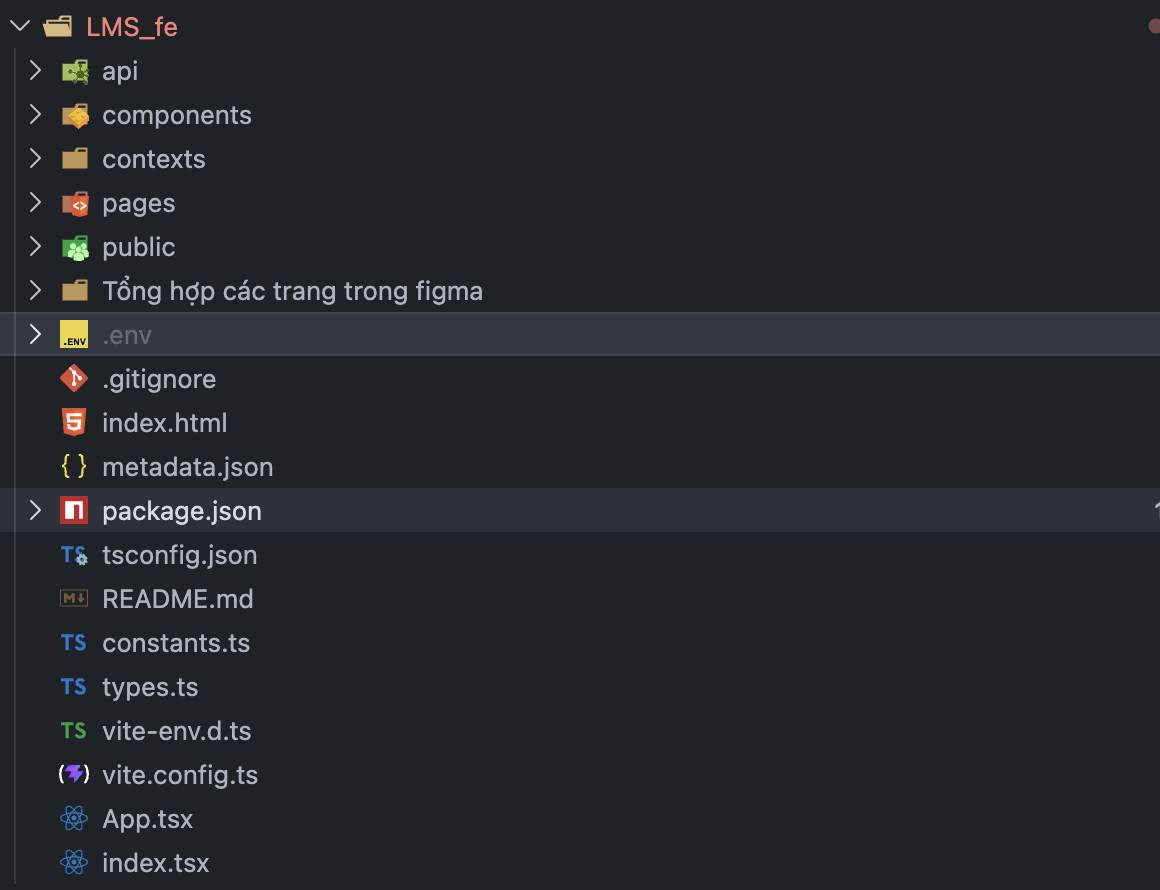
\includegraphics[width=0.5\textwidth]{picture/cautruc/LMS-FE.png}
    \caption{Cấu trúc thư mục mã nguồn Frontend}
    \label{fig:source_fe}
\end{figure}

\noindent\textbf{Mô tả cấu trúc:}
Frontend được xây dựng dựa trên ReactJS và trình đóng gói Vite. Các thành phần chính bao gồm:
\begin{itemize}
    \item \texttt{api/}: Chứa các cấu hình Axios và các hàm gọi API giao tiếp với Backend.
    \item \texttt{components/}: Nơi lưu trữ các thành phần giao diện (UI components) có thể tái sử dụng trên nhiều trang.
    \item \texttt{contexts/}: Quản lý trạng thái toàn cục của ứng dụng (Context API) như thông tin người dùng, trạng thái đăng nhập, giỏ sách/wishlist.
    \item \texttt{pages/}: Chứa mã nguồn của các trang màn hình chính (Trang chủ, Đăng nhập, Chi tiết sách, Dashboard...).
\end{itemize}

\subsection{Mã nguồn Backend (Máy chủ ứng dụng)}

\begin{figure}[H]
    \centering
    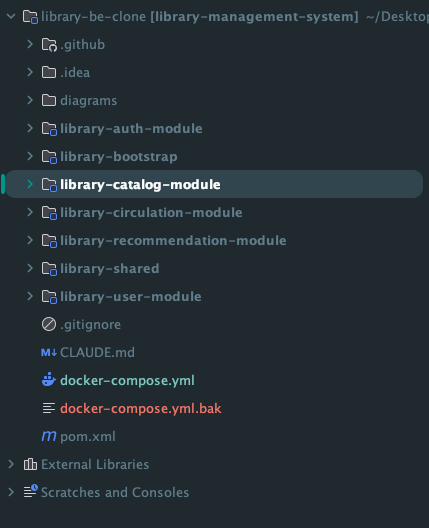
\includegraphics[width=0.5\textwidth]{picture/cautruc/LMS-BE.png}
    \caption{Cấu trúc thư mục mã nguồn Backend (Modular Monolith)}
    \label{fig:source_be}
\end{figure}

\noindent\textbf{Mô tả cấu trúc:}
Backend được phát triển bằng Java Spring Boot, áp dụng kiến trúc Modular Monolith để chia tách các nghiệp vụ lõi thành từng mô-đun riêng biệt:
\begin{itemize}
    \item \texttt{library-auth-module}: Xử lý toàn bộ logic xác thực (Authentication), phân quyền (Authorization) và tích hợp SSO (Google Login).
    \item \texttt{library-catalog-module}: Quản lý thông tin metadata của ấn phẩm, sách vật lý, tác giả và danh mục.
    \item \texttt{library-circulation-module}: Xử lý các nghiệp vụ vòng đời tài liệu như mượn sách, trả sách, đặt trước và tính phí phạt.
    \item \texttt{library-recommendation-module}: Cung cấp các giao tiếp và logic nền tảng để kết nối với AI Module.
    \item \texttt{library-user-module}: Quản lý thông tin hồ sơ (Profile) của độc giả và thủ thư.
\end{itemize}

\subsection{Mã nguồn AI Module (Trí tuệ nhân tạo)}

\begin{figure}[H]
    \centering
    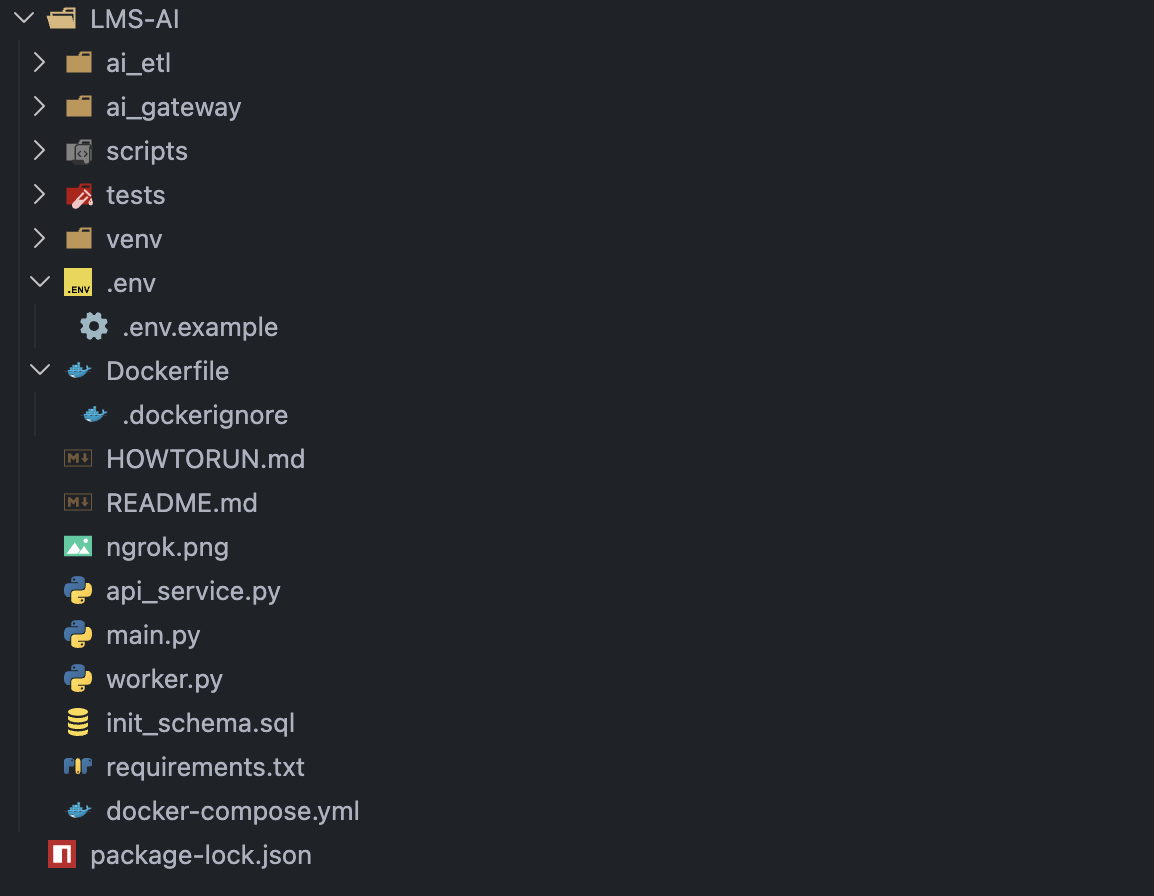
\includegraphics[width=0.5\textwidth]{picture/cautruc/LMS-AI.png}
    \caption{Cấu trúc thư mục mã nguồn phân hệ AI}
    \label{fig:source_ai}
\end{figure}

\noindent\textbf{Mô tả cấu trúc:}
Phân hệ Trí tuệ nhân tạo được viết bằng Python, cung cấp sức mạnh tìm kiếm ngữ nghĩa và gợi ý sách:
\begin{itemize}
    \item \texttt{ai\_etl/}: Chứa các đoạn mã thực thi ETL (Extract, Transform, Load) để trích xuất dữ liệu từ cơ sở dữ liệu chính, tiền xử lý và nhúng (embedding) để đưa vào Vector Database.
    \item \texttt{ai\_gateway/}: Khối giao tiếp API (thường dùng FastAPI) để tiếp nhận yêu cầu từ Backend Java.
    \item \texttt{scripts/}: Các tập lệnh tiện ích hỗ trợ huấn luyện (train) mô hình hoặc cập nhật dữ liệu.
    \item \texttt{api\_service.py} \& \texttt{worker.py}: Các tệp tin thực thi chính (entry points) để chạy dịch vụ AI và xử lý các tác vụ nền (background jobs).
    \item \texttt{docker-compose.yml} \& \texttt{Dockerfile}: Cấu hình đóng gói ứng dụng (Containerization) giúp việc triển khai lên môi trường máy chủ diễn ra tự động và đồng nhất.
\end{itemize}


\subsection{Hiện thực AI}

\subsubsection{Kiến trúc hệ thống AI}

Hệ thống AI của LMS được xây dựng dựa trên 2 thành phần chính: (1) ETL Pipeline xử lý sách, và (2) FastAPI Gateway cung cấp API cho tìm kiếm ngữ nghĩa và gợi ý sách.

\paragraph{ETL Pipeline (Extract-Transform-Load)}

Pipeline ETL được tối ưu hóa theo mô hình Map-Reduce:

\begin{itemize}
    \item \textbf{Extract}: Tải file PDF từ URL (lưu trữ trên AWS S3)
    \item \textbf{Transform}: Chunking text với Sliding Window (\textit{chunk\_size}=1800, \textit{overlap}=150)
    \item \textbf{Map Phase}: Sinh embedding 768 chiều cho mỗi chunk bằng SBERT (\textit{bkai-foundation-models/vietnamese-bi-encoder})
    \item \textbf{Reduce Phase}: Chọn các chunk đại diện, gọi LLM Gemini 1 lần để tổng hợp metadata (summary, audience, tags)
    \item \textbf{Load}: Lưu vectors vào \textit{ai\_engine.publication\_vectors} và tags vào bảng nối \textit{publication\_tags}
\end{itemize}

Tối ưu hóa: Sử dụng hash file PDF để skip xử lý lại, batch insert vectors (256 records/batch), connection pooling PostgreSQL.

\paragraph{AI Gateway API}

Cung cấp 2 endpoint chính:

\begin{enumerate}
    \item \textbf{Tìm kiếm ngữ nghĩa} (\texttt{POST /api/v1/semantic-search})
    \begin{itemize}
        \item Nhập: query text (VD: ``AI là gì?'')
        \item Xử lý: Mã hóa query thành vector, tính cosine similarity với pgvector
        \item Kết quả: Danh sách sách phù hợp nhất với query
    \end{itemize}
    
    \item \textbf{Gợi ý sách} (\texttt{POST /api/v1/recommendations})
    \begin{itemize}
        \item Nhập: user\_id
        \item Xử lý: Sử dụng mô hình ALS (Alternating Least Squares) trên ma trận user-item interactions
        \item Fallback: Cold-start strategy khi user mới (gợi ý sách được xem nhiều nhất)
    \end{itemize}
\end{enumerate}

\subsubsection{Công nghệ sử dụng}

\begin{table}[h]
    \centering
    \begin{tabular}{|l|l|}
    \hline
    \textbf{Thành phần} & \textbf{Công nghệ} \\
    \hline
    Embedding Model & SBERT (768 chiều) \\
    \hline
    Vector Database & PostgreSQL + pgvector \\
    \hline
    LLM & Google Gemini 2.5 (Flash \& Pro) \\
    \hline
    Web Framework & FastAPI + Uvicorn \\
    \hline
    Recommendation & Implicit ALS \\
    \hline
    PDF Processing & pypdf \\
    \hline
    \end{tabular}
    \caption{Stack công nghệ AI}
\end{table}

\subsubsection{API Documentation}

Hình \ref{fig:semantic_search} và \ref{fig:recommendations} trình bày Swagger documentation của hai endpoint chính:

\begin{figure}[H]
    \centering
    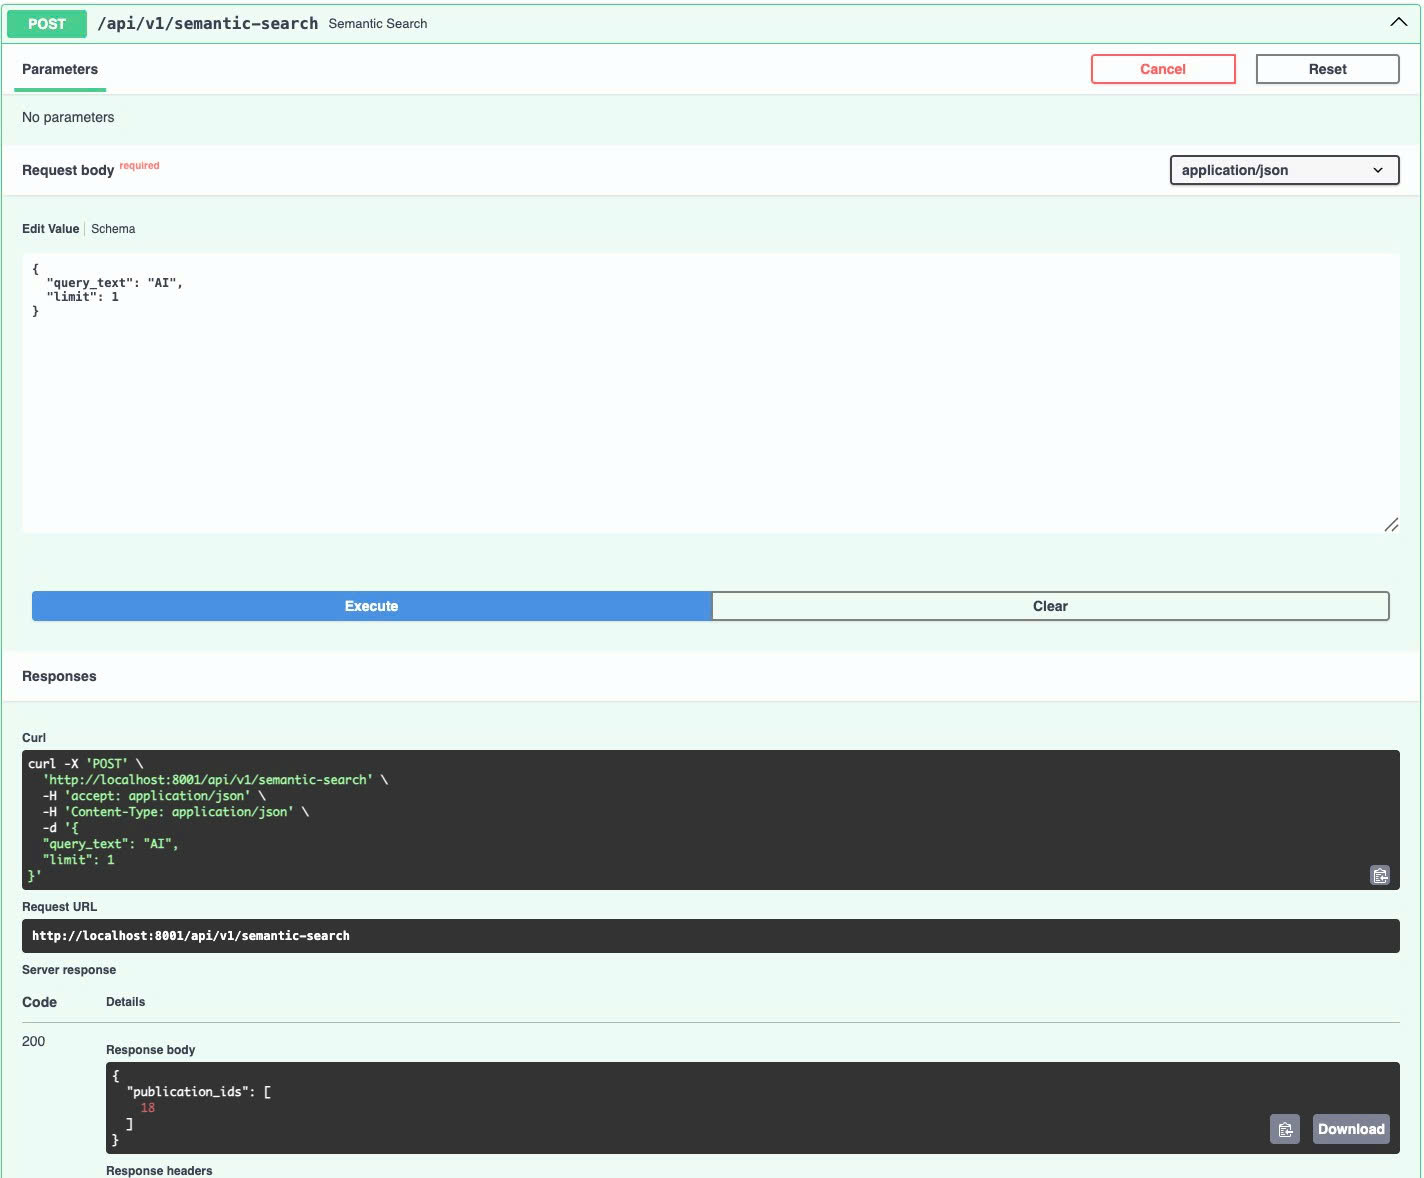
\includegraphics[width=0.9\textwidth]{picture/semantic.jpg}
    \caption{Endpoint tìm kiếm ngữ nghĩa}
    \label{fig:semantic_search}
\end{figure}

\begin{figure}[H]
    \centering
    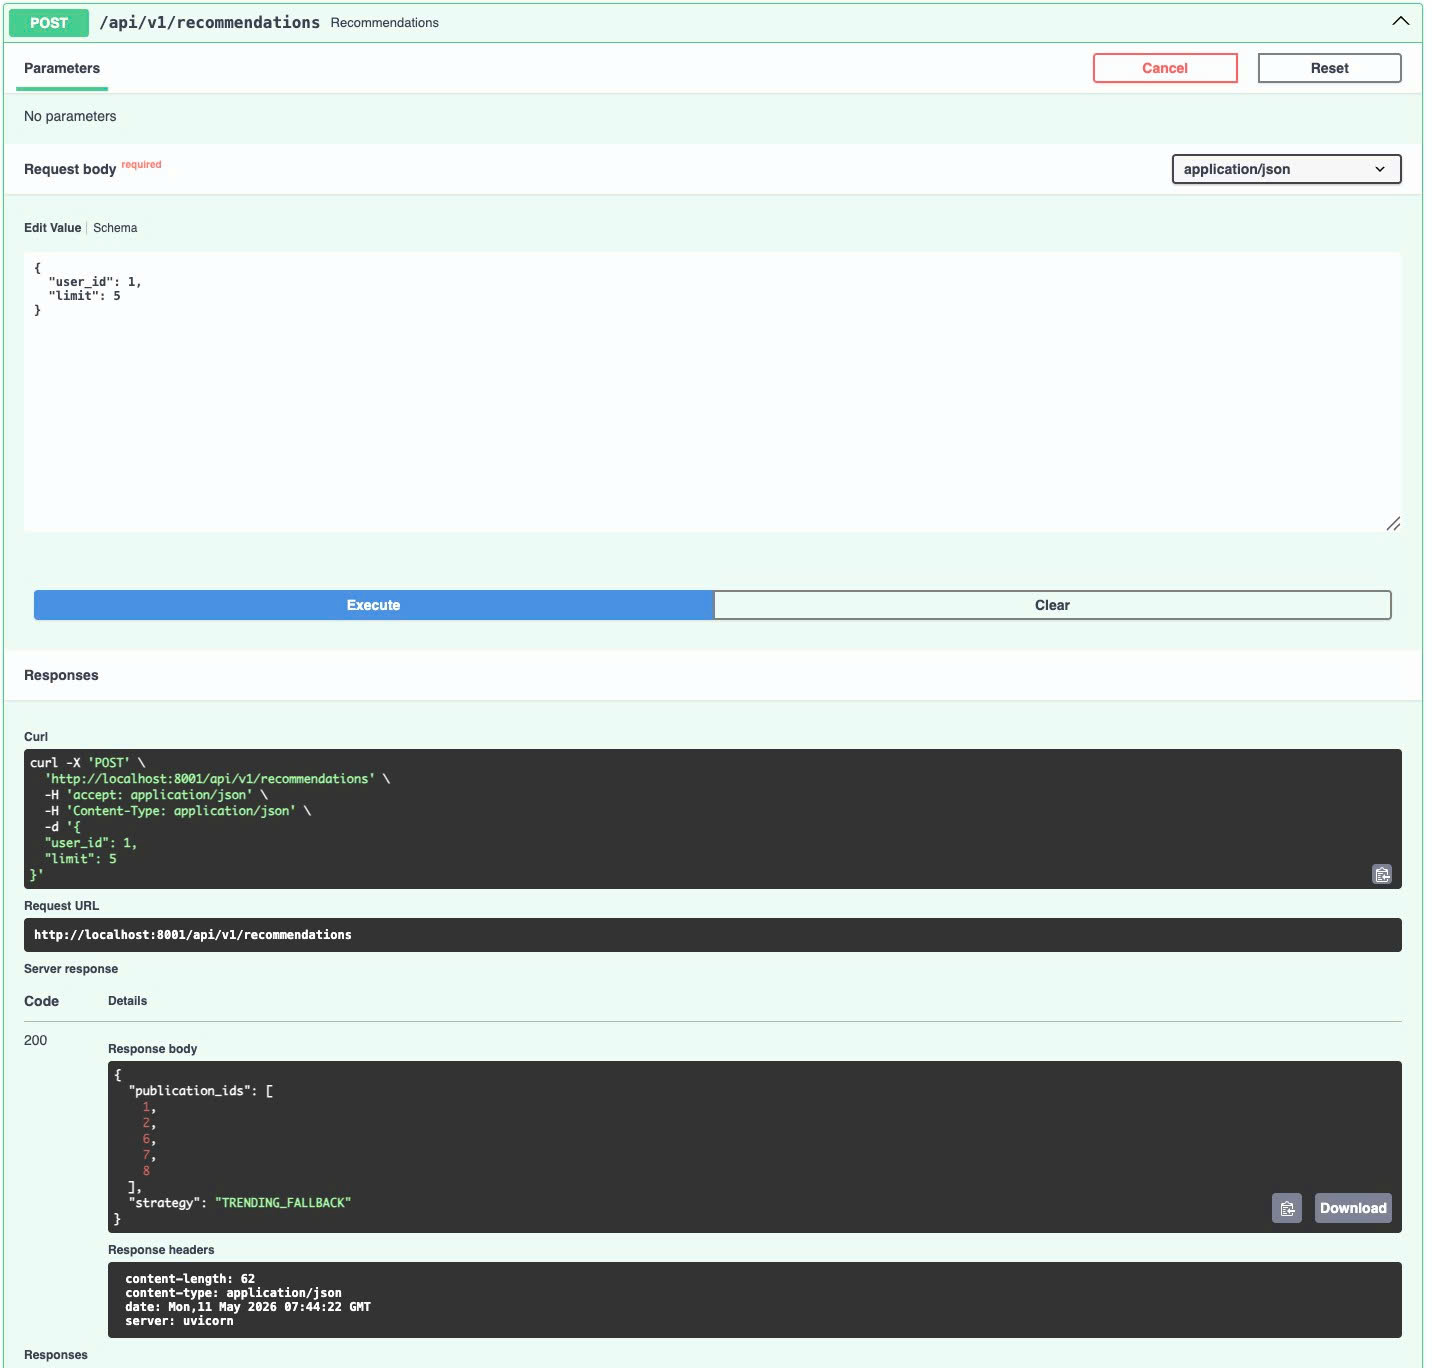
\includegraphics[width=0.9\textwidth]{picture/recommendation.jpg}
    \caption{Endpoint gợi ý sách}
    \label{fig:recommendations}
\end{figure}

\paragraph{Hiệu suất}

\begin{itemize}
    \item Semantic search: $<200$ms (với 10K vectors)
    \item Recommendations: $<500$ms (ALS inference)
    \item ETL processing: $\sim 2$-5 phút/sách (tùy kích thước PDF)
\end{itemize}

\subsubsection{Kết quả}

Sau khi chạy ETL cho 5 ấn phẩm, hệ thống đã:
\begin{itemize}
    \item Sinh \textbf{1,245 vectors} (768 chiều) từ PDF chunks
    \item Tạo \textbf{5 tags} tổng hợp bằng LLM
    \item Chuẩn bị cơ sở dữ liệu cho semantic search và recommendations
\end{itemize}




\section{Danh sách hiện thực chức năng theo API}

\subsection{Đăng ký và Xác thực tài khoản}

\subsubsection{Giao diện Đăng ký tài khoản}

\begin{figure}[H]
    \centering
    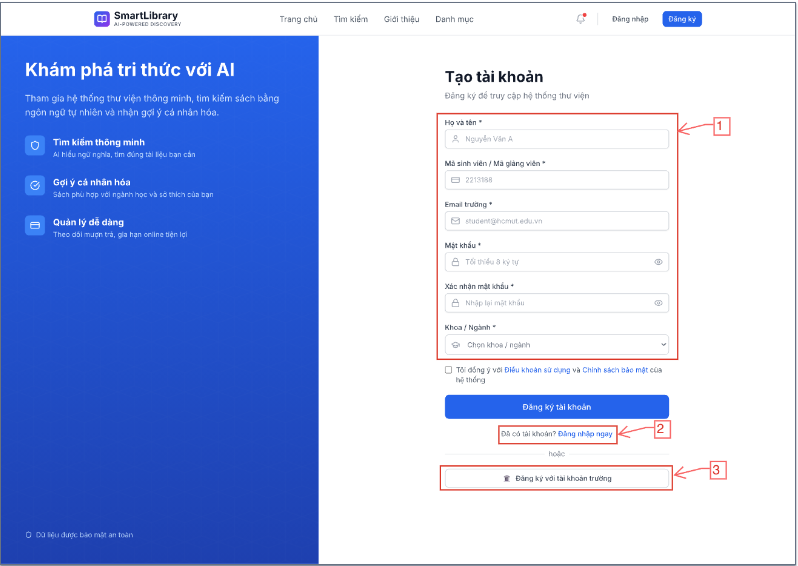
\includegraphics[width=0.85\textwidth]{picture/dangky/1.png}
    \caption{Giao diện Đăng ký tài khoản hệ thống SmartLibrary}
    \label{fig:register_ui}
\end{figure}

\noindent\textbf{Chú thích các vùng chức năng:}
\begin{itemize}
    \item \textbf{Vùng 1 (Biểu mẫu đăng ký):} Khu vực người dùng nhập các thông tin cá nhân và định danh bao gồm: Họ và tên, Mã sinh viên (hoặc Mã giảng viên), Email trường, Mật khẩu, và Khoa/Ngành trực thuộc.
    \item \textbf{Vùng 2 (Chuyển hướng đăng nhập):} Liên kết hỗ trợ người dùng chuyển nhanh sang trang Đăng nhập nếu đã có tài khoản từ trước.
    \item \textbf{Vùng 3 (Đăng nhập SSO):} Tùy chọn đăng ký/đăng nhập nhanh thông qua hệ thống tài khoản chung (SSO) của nhà trường.
\end{itemize}

\vspace{0.5cm}
\noindent\textbf{Đặc tả API Đăng ký tài khoản (User Registration):}
\begin{itemize}
    \item \textbf{Endpoint:} \texttt{POST /api/v1/auth/register}
    \item \textbf{Định dạng dữ liệu:} \texttt{application/json}
    \item \textbf{Mô tả:} Tiếp nhận thông tin đăng ký từ sinh viên, khởi tạo tài khoản và kích hoạt quy trình xác thực email. Hệ thống áp dụng kiểm soát dữ liệu (Validation) chặt chẽ tại tầng Application.
\end{itemize}

\begin{table}[H]
    \centering
    \caption{Đặc tả dữ liệu đầu vào (Request Body)}
    \renewcommand{\arraystretch}{1.3}
    \begin{tabularx}{\textwidth}{|l|l|X|X|}
        \hline
        \textbf{Trường dữ liệu} & \textbf{Kiểu} & \textbf{Ràng buộc kỹ thuật (Validation)} & \textbf{Ý nghĩa nghiệp vụ} \\ \hline
        fullName & String & @Pattern (Chỉ chứa chữ và khoảng trắng) & Tên đầy đủ của sinh viên. \\ \hline
        studentId & String & @Pattern (Đúng 7 chữ số) & Mã số sinh viên chính quy. \\ \hline
        email & String & @Pattern (Đuôi @hcmut.edu.vn) & Email định danh do nhà trường cấp. \\ \hline
        password & String & Tối thiểu 4 ký tự & Mật khẩu truy cập hệ thống. \\ \hline
        faculty & Enum & Thuộc danh sách Khoa hợp lệ & Khoa mà sinh viên đang theo học. \\ \hline
    \end{tabularx}
\end{table}

\noindent\textbf{Luồng xử lý nghiệp vụ (Business Logic):}
\begin{enumerate}
    \item \textbf{Kiểm tra điều kiện:} Hệ thống kiểm tra xem email đã được đăng ký trước đó hay chưa.
    \item \textbf{Khởi tạo tài khoản:} 
    \begin{itemize}
        \item Tài khoản mới mặc định được gán vai trò \texttt{STUDENT}.
        \item Trạng thái ban đầu là \texttt{INACTIVE} (Chưa kích hoạt).
        \item Thiết lập thông số mặc định: Điểm tín nhiệm (Credit Score) = 100 và bật tính năng đề xuất cá nhân hóa bằng AI.
    \end{itemize}
    \item \textbf{Xác thực:} Phát hành yêu cầu gửi email chứa mã kích hoạt (Token) đến địa chỉ sinh viên vừa cung cấp.
\end{enumerate}

\noindent\textbf{Giải pháp kỹ thuật và Kiến trúc (Technical Implementation):}
\begin{itemize}
    \item \textbf{Kiến trúc Domain-Driven Design (DDD):} Logic đăng ký được đóng gói gọn trong \texttt{SignUpUseCase}. Thực thể \texttt{User} tự quản lý trạng thái và phát sinh Domain Event (\texttt{UserRegisteredEvent}) khi có thay đổi quan trọng.
    \item \textbf{Bảo mật dữ liệu:} Sử dụng \texttt{PasswordHasher} (Interface) để trừu tượng hóa thuật toán mã hóa (BCrypt/Argon2), đảm bảo không lưu mật khẩu dưới dạng văn bản thuần túy (Plaintext).
    \item \textbf{Xử lý bất đồng bộ với Kafka (Event-Driven):} Sau khi lưu User thành công, một sự kiện được đẩy vào Kafka topic \texttt{user.registered}. Dịch vụ Email (Consumer) sẽ lắng nghe để gửi thư, giúp giảm thời gian phản hồi (Response time) và tách biệt logic (Decoupling).
    \item \textbf{Quản lý giao dịch (Transaction):} Dùng \texttt{@Transactional} đảm bảo tính nhất quán (ACID). Nếu lưu DB lỗi, sự kiện gửi email sẽ không được phát đi.
\end{itemize}


\noindent\textbf{Cấu trúc phản hồi (Response Format):}
\begin{itemize}
    \item \textbf{Thành công (200 OK):}
\begin{verbatim}
{
  "status": "success",
  "message": "Register successful",
  "data": null
}
\end{verbatim}
    \item \textbf{Lỗi nghiệp vụ (409 Conflict - Trùng Email):}
\begin{verbatim}
{
  "status": "error",
  "message": "Email already exists",
  "code": "EMAIL_ALREADY_EXISTS"
}
\end{verbatim}
\end{itemize}

\subsubsection{Giao diện Xác thực Email và Hoàn tất}

\begin{figure}[H]
    \centering
    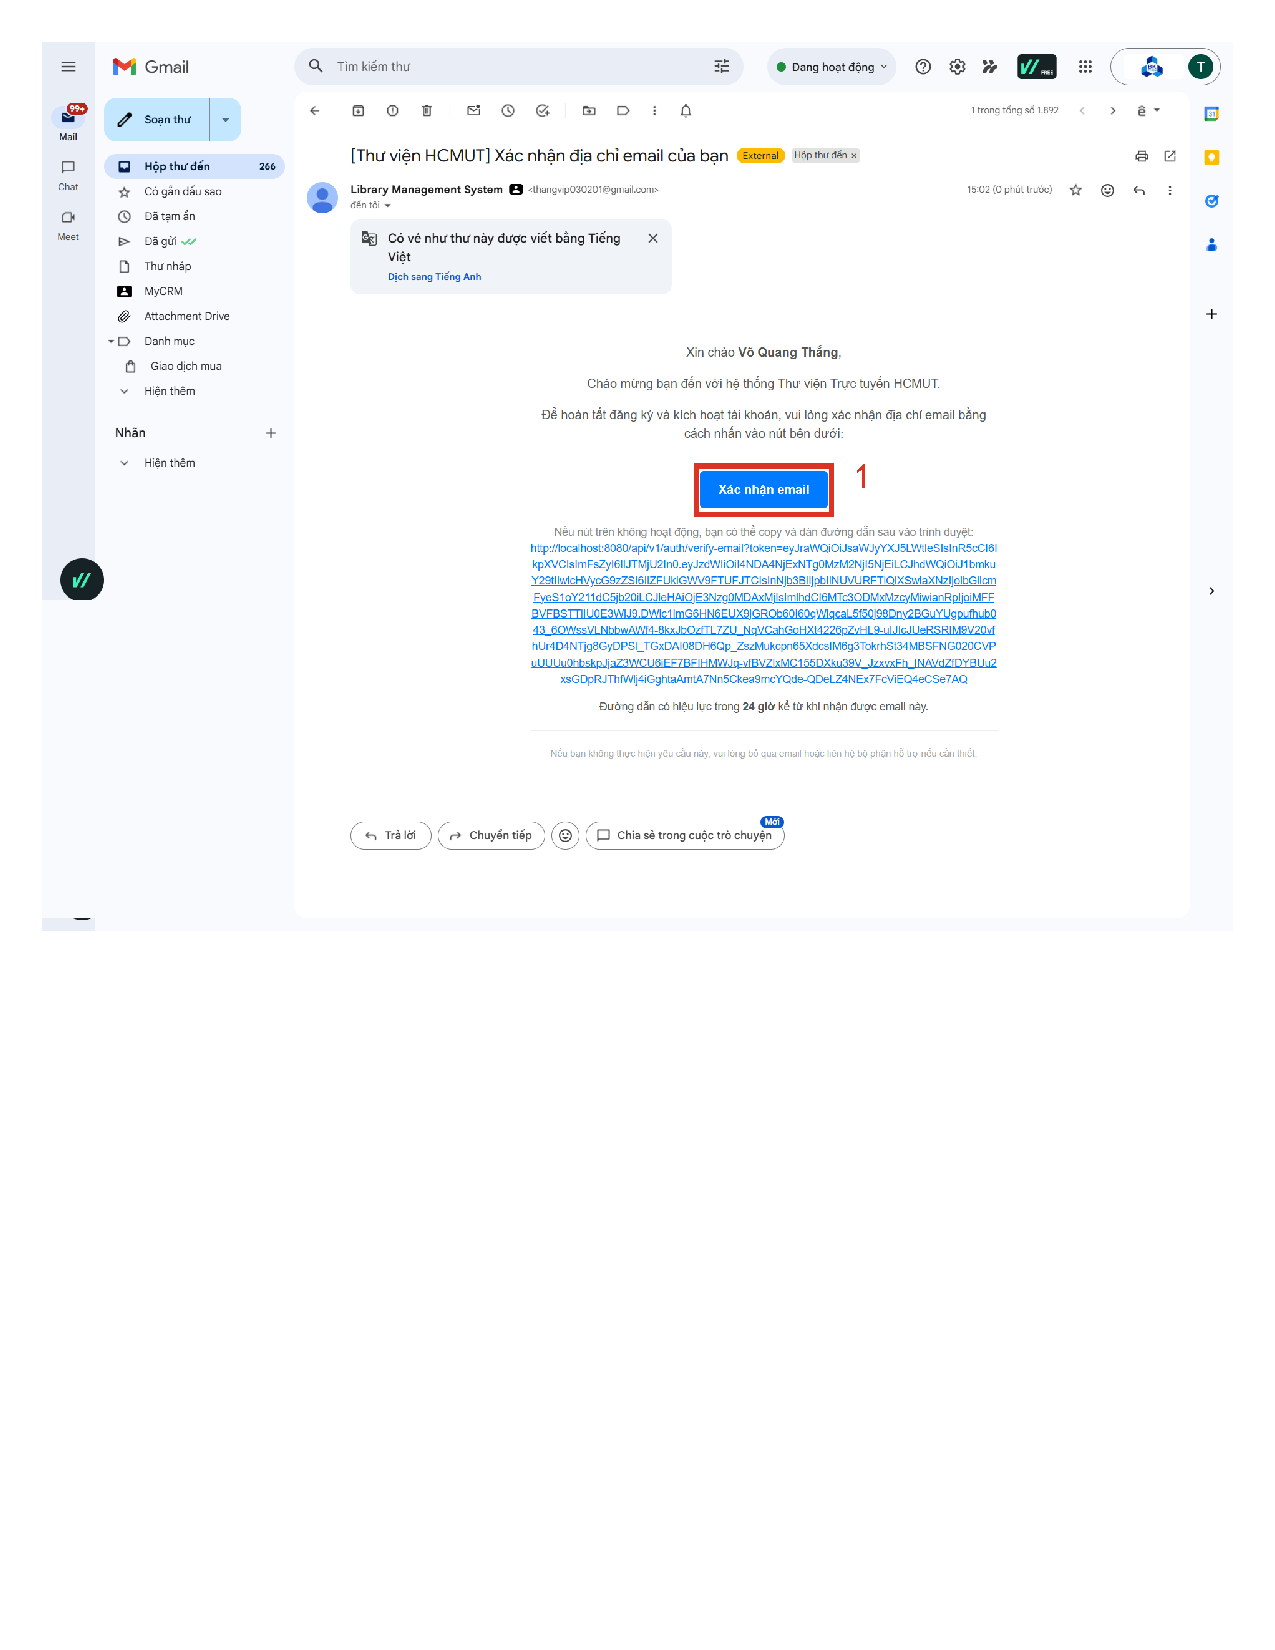
\includegraphics[width=\textwidth]{picture/dangky/2.pdf}
    \caption{Nội dung Email yêu cầu xác nhận tài khoản}
    \label{fig:verify_email}
\end{figure}

\noindent\textbf{Chú thích giao diện:} 
\begin{itemize}
    \item \textbf{Vùng 1 (Nút thao tác chính):} Nút bấm chứa đường dẫn đính kèm mã token bảo mật (JWT/UUID) để kích hoạt tài khoản một cách tự động.
    \item \textbf{Vùng 2 (Đường dẫn dự phòng):} Đường dẫn thô được cung cấp phòng trường hợp nút bấm ở Vùng 1 bị trình duyệt hoặc ứng dụng mail chặn chuyển hướng.
\end{itemize}

\begin{figure}[H]
    \centering
    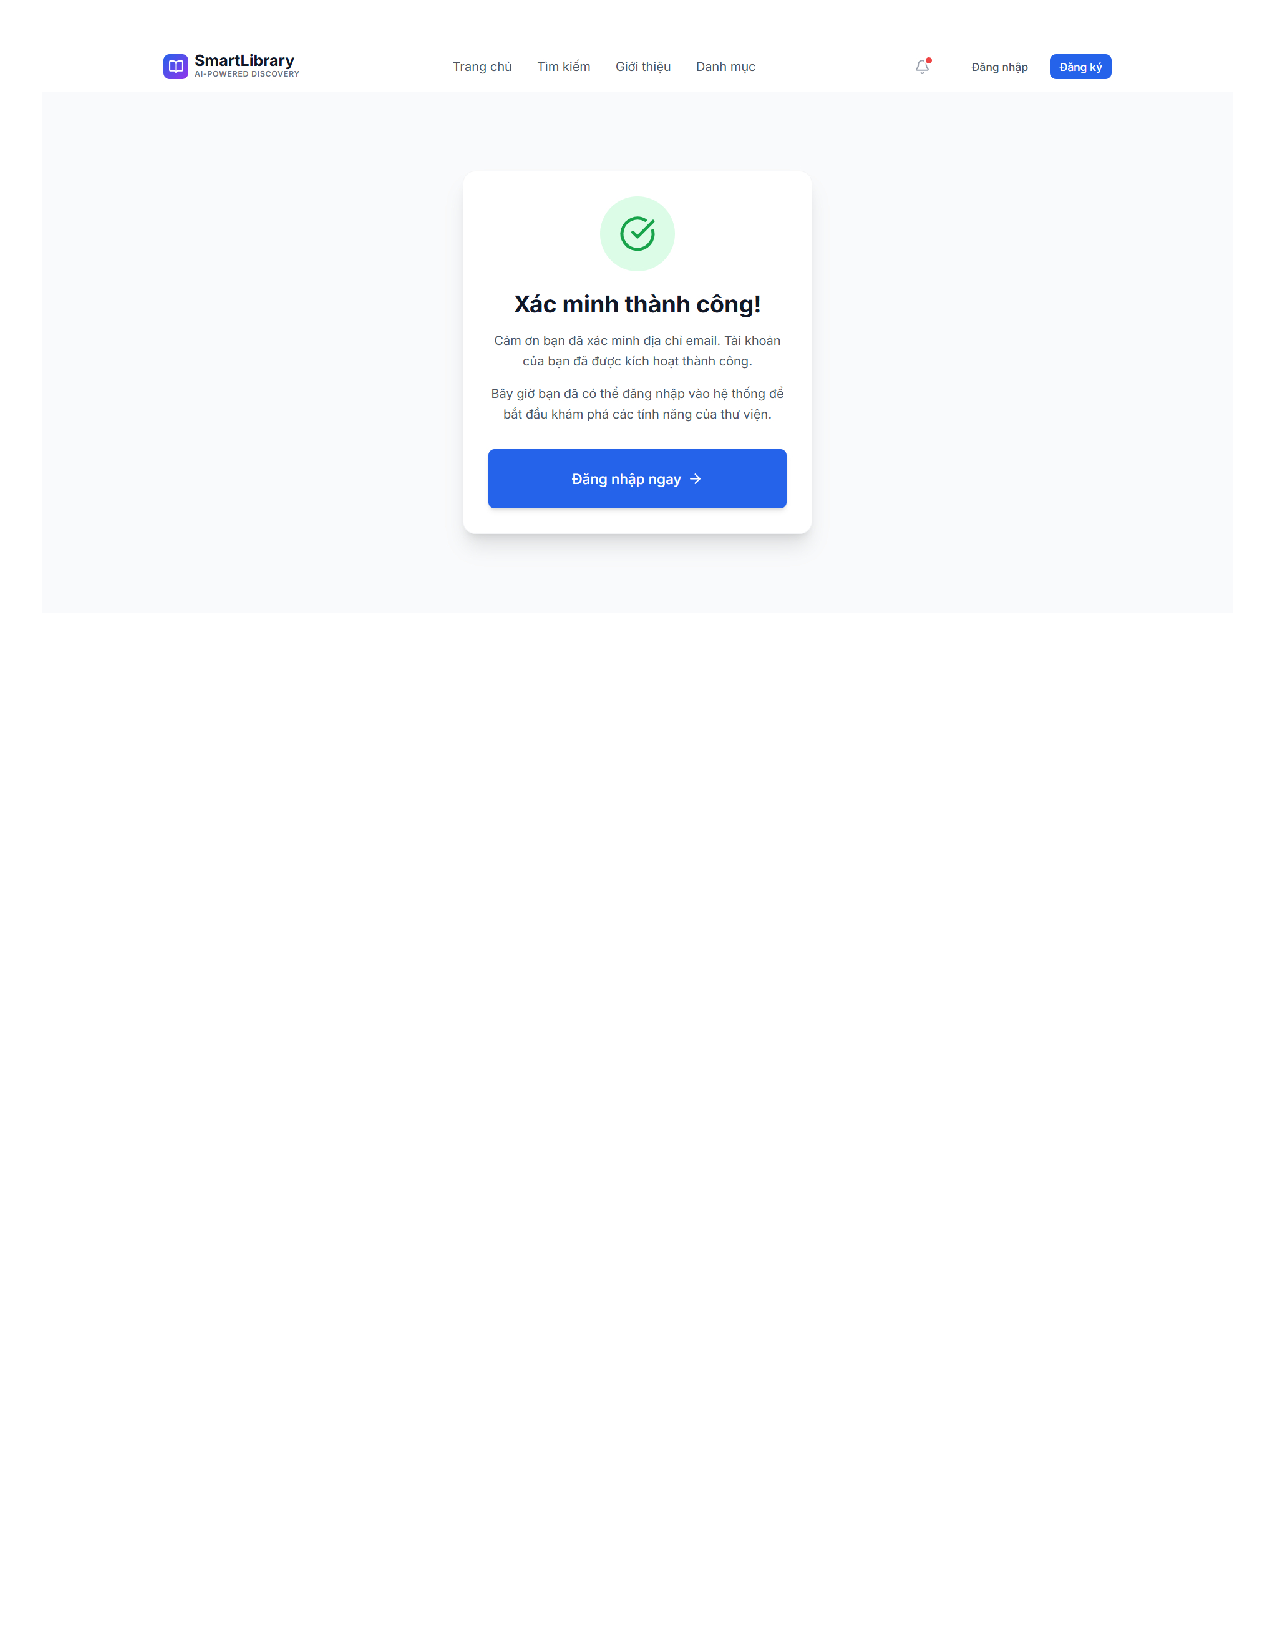
\includegraphics[width=0.85\textwidth]{picture/dangky/3.pdf}
    \caption{Giao diện thông báo kích hoạt tài khoản thành công}
    \label{fig:verify_success}
\end{figure}

\noindent\textbf{Mô tả nghiệp vụ:} Khi người dùng truy cập vào liên kết xác thực hợp lệ, hệ thống sẽ kiểm tra chữ ký và hạn mức thời gian của token. Nếu hợp lệ, trạng thái của \texttt{User} trong Database sẽ được chuyển từ \texttt{INACTIVE} sang \texttt{ACTIVE}, và giao diện thông báo thành công sẽ hiển thị cùng với nút điều hướng người dùng đăng nhập.
% Preamble cần thiết: \usepackage{graphicx}, \usepackage{float}, \usepackage{tabularx}, \usepackage{booktabs}


% Preamble cần thiết: \usepackage{graphicx}, \usepackage{float}, \usepackage{tabularx}, \usepackage{booktabs}, \usepackage{verbatim}

\subsection{Đăng nhập hệ thống}

\subsubsection{Giao diện Đăng nhập}

\begin{figure}[H]
    \centering
    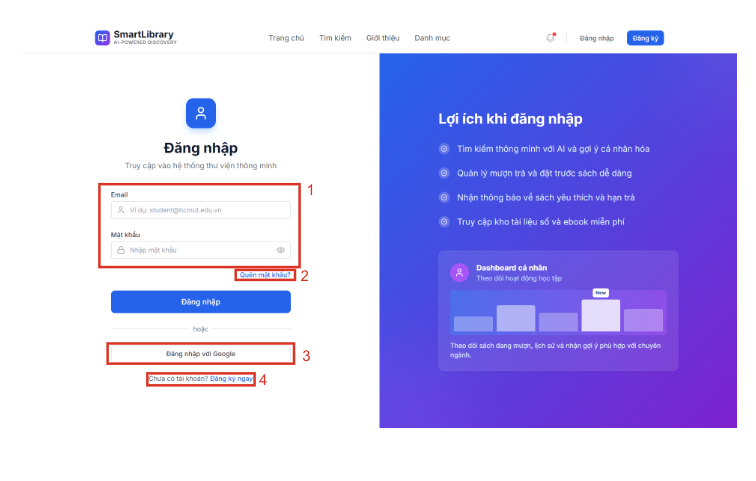
\includegraphics[width=0.85\textwidth]{picture/dangnhapbinhthuong/login.png}
    \caption{Giao diện Đăng nhập hệ thống SmartLibrary}
    \label{fig:login_ui}
\end{figure}

\noindent\textbf{Chú thích các vùng chức năng:}
\begin{itemize}
    \item \textbf{Vùng 1 (Biểu mẫu đăng nhập):} Khu vực người dùng nhập thông tin xác thực bao gồm Email trường (theo định dạng @hcmut.edu.vn) và Mật khẩu.
    \item \textbf{Vùng 2 (Quên mật khẩu):} Liên kết hỗ trợ người dùng thao tác khôi phục lại mật khẩu trong trường hợp thất lạc hoặc quên.
    \item \textbf{Vùng 3 (Đăng nhập SSO):} Tùy chọn đăng nhập nhanh thông qua hệ thống tài khoản Google của nhà trường.
    \item \textbf{Vùng 4 (Chuyển hướng đăng ký):} Liên kết điều hướng người dùng sang trang Đăng ký nếu chưa có tài khoản trên hệ thống.
\end{itemize}

\vspace{0.5cm}
\subsubsection{Đặc tả luồng nghiệp vụ Đăng nhập}

Mục tiêu của luồng nghiệp vụ này là đảm bảo xác thực đúng danh tính người dùng, kiểm tra trạng thái hoạt động của tài khoản và tiến hành phân quyền truy cập ngay sau khi đăng nhập thành công. Luồng đăng nhập được chia thành 4 giai đoạn chính:

\noindent\textbf{1. Giai đoạn 1: Tiếp nhận và Kiểm tra định dạng (Frontend)}
\begin{itemize}
    \item Người dùng cung cấp thông tin gồm Email và Mật khẩu thông qua giao diện đăng nhập.
    \item Hệ thống thực hiện kiểm tra sơ bộ: Email phải đúng định dạng của trường. Nếu không hợp lệ, hệ thống sẽ báo lỗi ngay tại giao diện mà chưa gửi yêu cầu về máy chủ nhằm tối ưu tài nguyên.
\end{itemize}

\noindent\textbf{2. Giai đoạn 2: Xác thực và Kiểm tra điều kiện tài khoản (Backend)}
\begin{itemize}
    \item \textbf{Tìm kiếm tài khoản:} Hệ thống truy vấn thông tin người dùng trong cơ sở dữ liệu dựa trên Email.
    \item \textbf{Kiểm tra trạng thái tài khoản (Nghiệp vụ quan trọng):} Trước khi kiểm tra mật khẩu, hệ thống xác minh trạng thái hoạt động:
    \begin{itemize}
        \item \textit{Tài khoản chưa kích hoạt:} Hệ thống từ chối đăng nhập và yêu cầu người dùng kiểm tra hộp thư để xác thực.
        \item \textit{Tài khoản bị khóa/cấm:} Ngăn chặn truy cập và thông báo lý do cụ thể (áp dụng cho tài khoản vi phạm nội quy hoặc bị khóa thủ công bởi quản trị viên).
    \end{itemize}
    \item \textbf{Xác thực mật khẩu:} Hệ thống sử dụng thuật toán mã hóa một chiều để so sánh mật khẩu nhập vào với mã băm (hash) đã lưu trong cơ sở dữ liệu.
\end{itemize}

\noindent\textbf{3. Giai đoạn 3: Khởi tạo phiên làm việc và Phân quyền}
\begin{itemize}
    \item \textbf{Cấp phát Token:} Sau khi xác thực thành công, máy chủ tạo ra bộ định danh bảo mật (gồm Access Token và Refresh Token) để duy trì trạng thái đăng nhập.
    \item \textbf{Phân quyền người dùng (Role-based):} Thông tin quyền hạn được đính kèm vào token:
    \begin{itemize}
        \item \textit{Quyền Thủ thư (Librarian):} Có toàn quyền quản lý kho sách, duyệt yêu cầu mượn trả và xem báo cáo.
        \item \textit{Quyền Sinh viên (Student):} Có quyền tìm kiếm sách, đặt trước và quản lý thông tin mượn trả cá nhân.
    \end{itemize}
\end{itemize}

\noindent\textbf{4. Giai đoạn 4: Điều hướng người dùng (Frontend)}
\begin{itemize}
    \item Hệ thống client nhận bộ định danh và lưu trữ bảo mật tại trình duyệt.
    \item Dựa trên quyền hạn đã được phân tích, hệ thống tự động điều hướng: Thủ thư được dẫn trực tiếp đến Bảng điều khiển quản lý (Librarian Dashboard), Sinh viên được dẫn đến Trang cá nhân và Khám phá sách (User Dashboard).
\end{itemize}

\vspace{0.5cm}


% Preamble cần thiết: \usepackage{graphicx}, \usepackage{float}, \usepackage{tabularx}, \usepackage{booktabs}, \usepackage{verbatim}

\subsection{Đăng nhập bằng Google }

\subsubsection{Giao diện Đăng nhập qua tài khoản Google}

\begin{figure}[H]
    \centering
    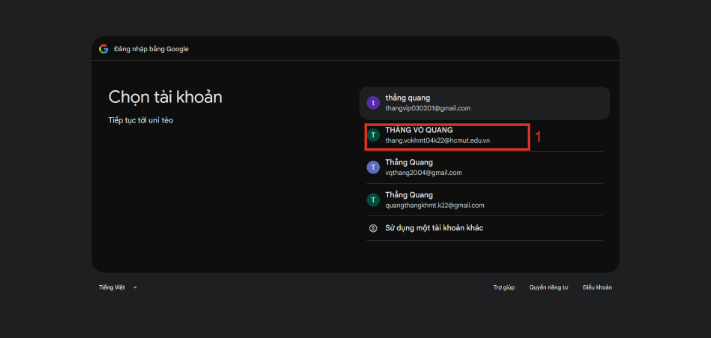
\includegraphics[width=0.85\textwidth]{picture/dangnhapvoigoogle/1.png}
    \caption{Giao diện lựa chọn tài khoản Google để xác thực}
    \label{fig:google_sso_select}
\end{figure}

\noindent\textbf{Chú thích giao diện:}
\begin{itemize}
    \item \textbf{Vùng 1 (Danh sách tài khoản):} Cửa sổ pop-up từ Google OAuth2 hiển thị các tài khoản đang lưu trên trình duyệt. Để vào được hệ thống, người dùng bắt buộc phải chọn tài khoản email có đuôi mở rộng hợp lệ của trường (ví dụ: \texttt{@hcmut.edu.vn}).
\end{itemize}

\begin{figure}[H]
    \centering
    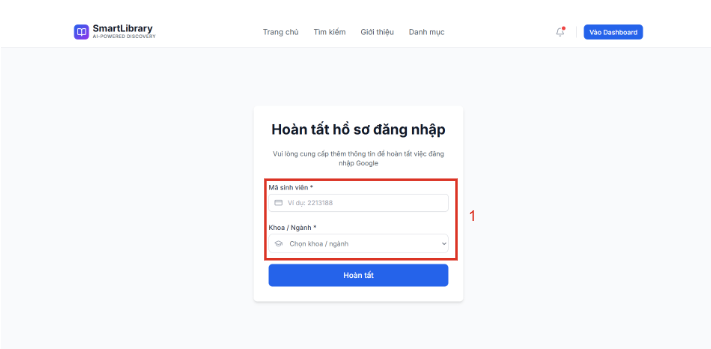
\includegraphics[width=0.85\textwidth]{picture/dangnhapvoigoogle/2.png}
    \caption{Giao diện hoàn tất hồ sơ cho lần đăng nhập đầu tiên}
    \label{fig:google_sso_complete}
\end{figure}

\noindent\textbf{Chú thích giao diện:}
\begin{itemize}
    \item \textbf{Vùng 1 (Biểu mẫu bổ sung thông tin):} Trong trường hợp người dùng đăng nhập bằng Google lần đầu, hệ thống chỉ lấy được Email, Tên và Ảnh đại diện. Màn hình này bắt buộc người dùng cung cấp thêm \textbf{Mã sinh viên} và \textbf{Khoa/Ngành} trước khi được cấp quyền truy cập vào bảng điều khiển (Dashboard).
\end{itemize}

\vspace{0.5cm}
\subsubsection{Đặc tả luồng nghiệp vụ và API}

Luồng đăng nhập bằng Google chia làm 2 nhánh chính: Đăng nhập thông thường (tài khoản đã tồn tại) và Khởi tạo tài khoản qua Google (lần đầu đăng nhập).

\vspace{0.3cm}
\noindent\textbf{1. API Xác thực Token từ Google (Xử lý Đăng nhập)}
\begin{itemize}
    \item \textbf{Endpoint:} \texttt{POST /api/v1/auth/google}
    \item \textbf{Quyền truy cập:} Public
    \item \textbf{Dữ liệu đầu vào:} \texttt{idToken} (Chuỗi token do Google SDK trả về sau khi người dùng chọn tài khoản).
    \item \textbf{Mô tả logic:}
    \begin{enumerate}
        \item Backend nhận \texttt{idToken} và xác minh chữ ký với Google Server (để chống giả mạo).
        \item Lấy địa chỉ email từ token. Kiểm tra định dạng email (phải là \texttt{@hcmut.edu.vn}).
        \item Kiểm tra email trong cơ sở dữ liệu (Database):
        \begin{itemize}
            \item \textit{Trường hợp 1 (Đã có tài khoản):} Hệ thống trực tiếp cấp phát Access Token / Refresh Token và trả về mã \texttt{200 OK}. Người dùng vào thẳng Dashboard.
            \item \textit{Trường hợp 2 (Tài khoản chưa tồn tại):} Hệ thống lưu tạm thông tin (Email, Tên, Avatar) vào bộ nhớ đệm (Redis) kèm một \texttt{temporaryToken}, trả về mã \texttt{202 Accepted} và yêu cầu Frontend điều hướng sang màn hình \textbf{Hoàn tất hồ sơ}.
        \end{itemize}
    \end{enumerate}
\end{itemize}

\vspace{0.3cm}
\noindent\textbf{2. API Hoàn tất hồ sơ (Dành cho lần đăng nhập đầu tiên)}
\begin{itemize}
    \item \textbf{Endpoint:} \texttt{POST /api/v1/auth/google/complete-profile}
    \item \textbf{Quyền truy cập:} Yêu cầu Bearer Token là \texttt{temporaryToken} đã cấp ở bước trên.
\end{itemize}

\begin{table}[H]
    \centering
    \caption{Cấu trúc dữ liệu yêu cầu (Request Body) hoàn tất hồ sơ}
    \renewcommand{\arraystretch}{1.3}
    \begin{tabularx}{\textwidth}{|l|l|c|X|}
        \hline
        \textbf{Trường dữ liệu} & \textbf{Kiểu} & \textbf{Bắt buộc} & \textbf{Mô tả} \\ \hline
        studentId & String & \checkmark & Mã số sinh viên (Kiểm tra trùng lặp trong DB). \\ \hline
        faculty & Enum & \checkmark & Khoa/Ngành trực thuộc. \\ \hline
    \end{tabularx}
\end{table}

\noindent\textbf{Logic xử lý hoàn tất hồ sơ:}
\begin{itemize}
    \item Hệ thống trích xuất thông tin Google từ bộ nhớ đệm (dựa vào \texttt{temporaryToken}).
    \item Kết hợp thông tin Google với \texttt{studentId} và \texttt{faculty} do người dùng cung cấp.
    \item Khởi tạo bản ghi \texttt{User} mới trong cơ sở dữ liệu với trạng thái \texttt{ACTIVE} (không cần gửi email xác thực vì Google đã đảm bảo email là thật).
    \item Cấp phát Access Token / Refresh Token chính thức.
\end{itemize}

\vspace{0.5cm}

% Preamble cần thiết: \usepackage{graphicx}, \usepackage{float}, \usepackage{tabularx}, \usepackage{booktabs}, \usepackage{verbatim}

% Preamble cần thiết: \usepackage{graphicx}, \usepackage{float}, \usepackage{tabularx}, \usepackage{booktabs}

\subsection{Khôi phục mật khẩu}

\subsubsection{Yêu cầu khôi phục mật khẩu}

\begin{figure}[H]
    \centering
    \begin{minipage}{0.48\textwidth}
        \centering
        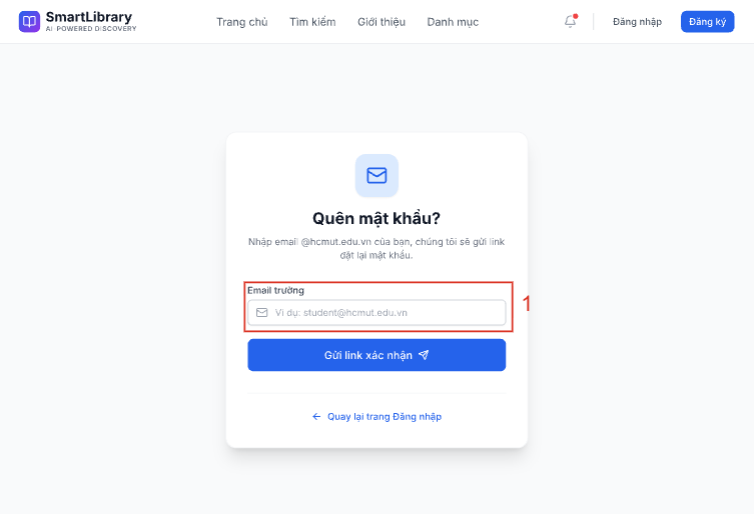
\includegraphics[width=\linewidth]{picture/quenmatkhau/1.png}
        \caption{Giao diện nhập email yêu cầu khôi phục}
        \label{fig:forgot_pwd_request}
    \end{minipage}\hfill
    \begin{minipage}{0.48\textwidth}
        \centering
        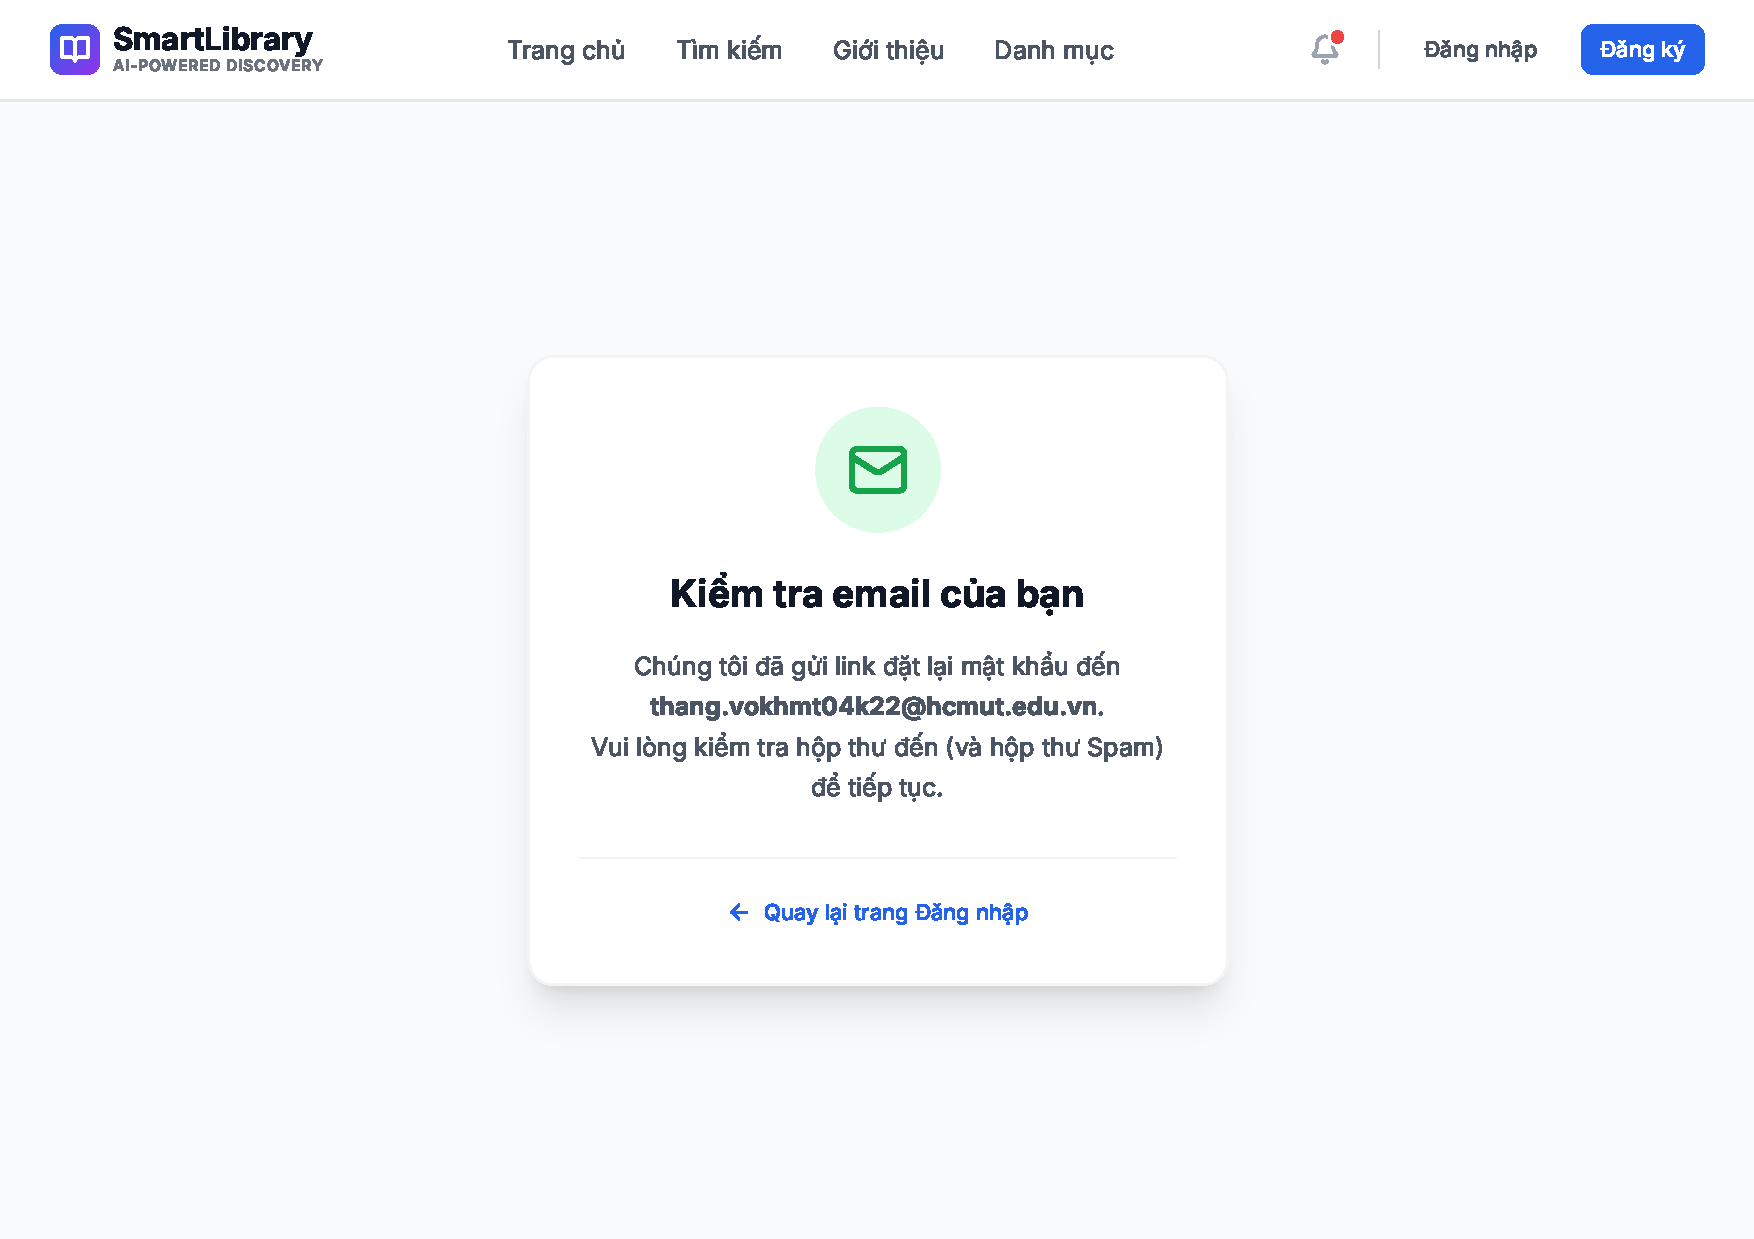
\includegraphics[width=\linewidth]{picture/quenmatkhau/2.pdf}
        \caption{Thông báo kiểm tra hộp thư}
        \label{fig:forgot_pwd_notice}
    \end{minipage}
\end{figure}

\noindent\textbf{Mô tả giao diện:} 
Khi người dùng quên thông tin truy cập, hệ thống cung cấp một biểu mẫu để nhập địa chỉ email định danh. Để đảm bảo tính hợp lệ, email đầu vào bắt buộc phải tuân thủ đúng định dạng tên miền do nhà trường cấp. Ngay sau khi gửi yêu cầu thành công, giao diện sẽ chuyển sang màn hình thông báo, hướng dẫn người dùng kiểm tra hộp thư đến hoặc thư mục rác để nhận đường dẫn xác thực.

\subsubsection{Xác thực hệ thống qua Email}

\begin{figure}[H]
    \centering
    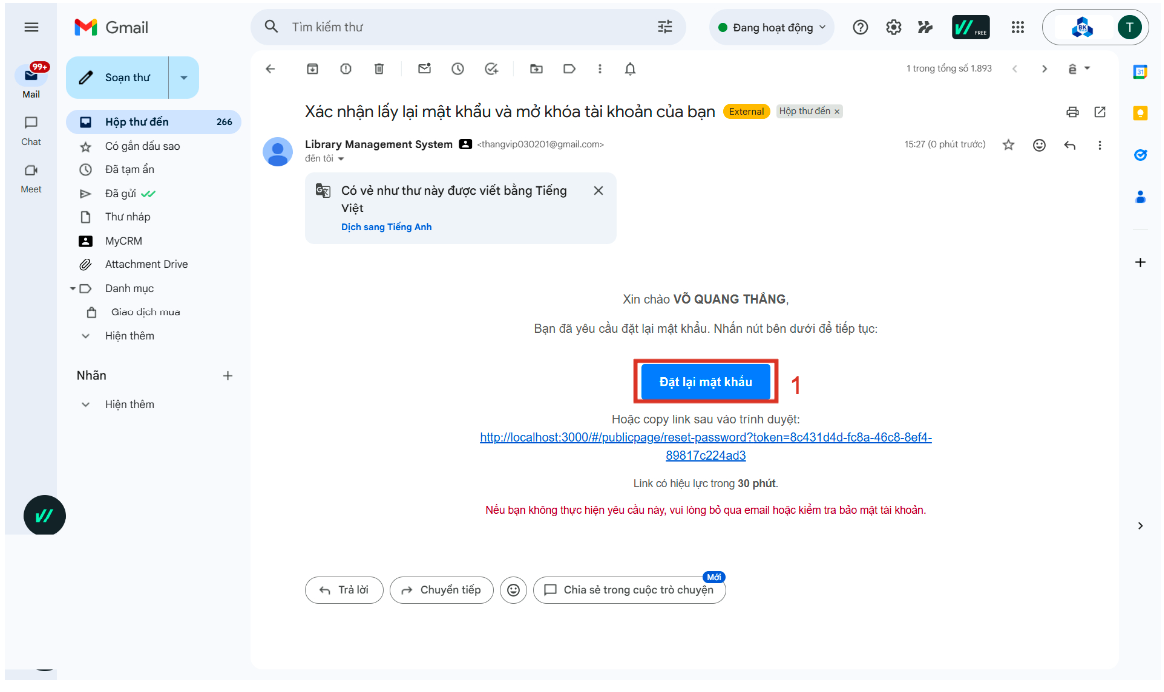
\includegraphics[width=\textwidth]{picture/quenmatkhau/3.png}
    \caption{Nội dung thư điện tử chứa đường dẫn đặt lại mật khẩu}
    \label{fig:forgot_pwd_email}
\end{figure}

\noindent\textbf{Mô tả giao diện:} 
Hệ thống tự động gửi một thư điện tử đến địa chỉ mà người dùng vừa cung cấp. Nội dung thư bao gồm một nút bấm chứa đường dẫn bảo mật để chuyển hướng đến trang thiết lập mật khẩu mới. Nhằm đảm bảo an toàn thông tin, đường dẫn này chỉ có hiệu lực sử dụng trong vòng 30 phút. Hệ thống cũng cung cấp đường dẫn dạng thô để người dùng sao chép trực tiếp vào trình duyệt trong trường hợp nút bấm bị lỗi.

\subsubsection{Thiết lập mật khẩu mới và Hoàn tất}

\begin{figure}[H]
    \centering
    \begin{minipage}{0.48\textwidth}
        \centering
        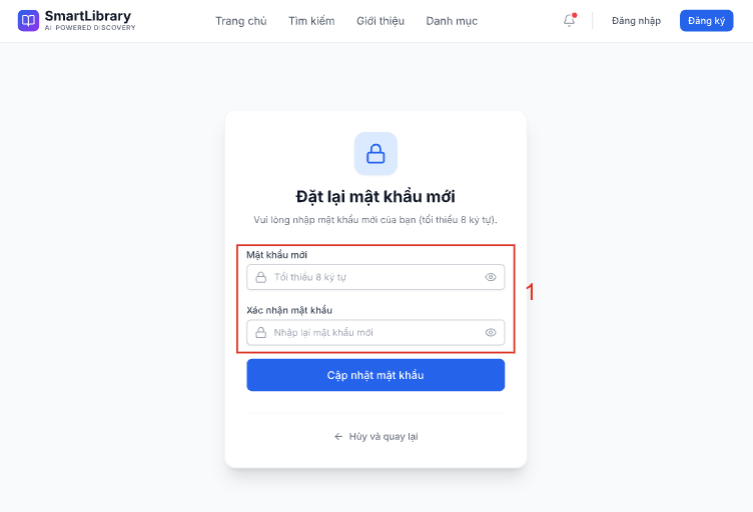
\includegraphics[width=\linewidth]{picture/quenmatkhau/4.png}
        \caption{Giao diện thiết lập mật khẩu mới}
        \label{fig:forgot_pwd_reset}
    \end{minipage}\hfill
    \begin{minipage}{0.48\textwidth}
        \centering
        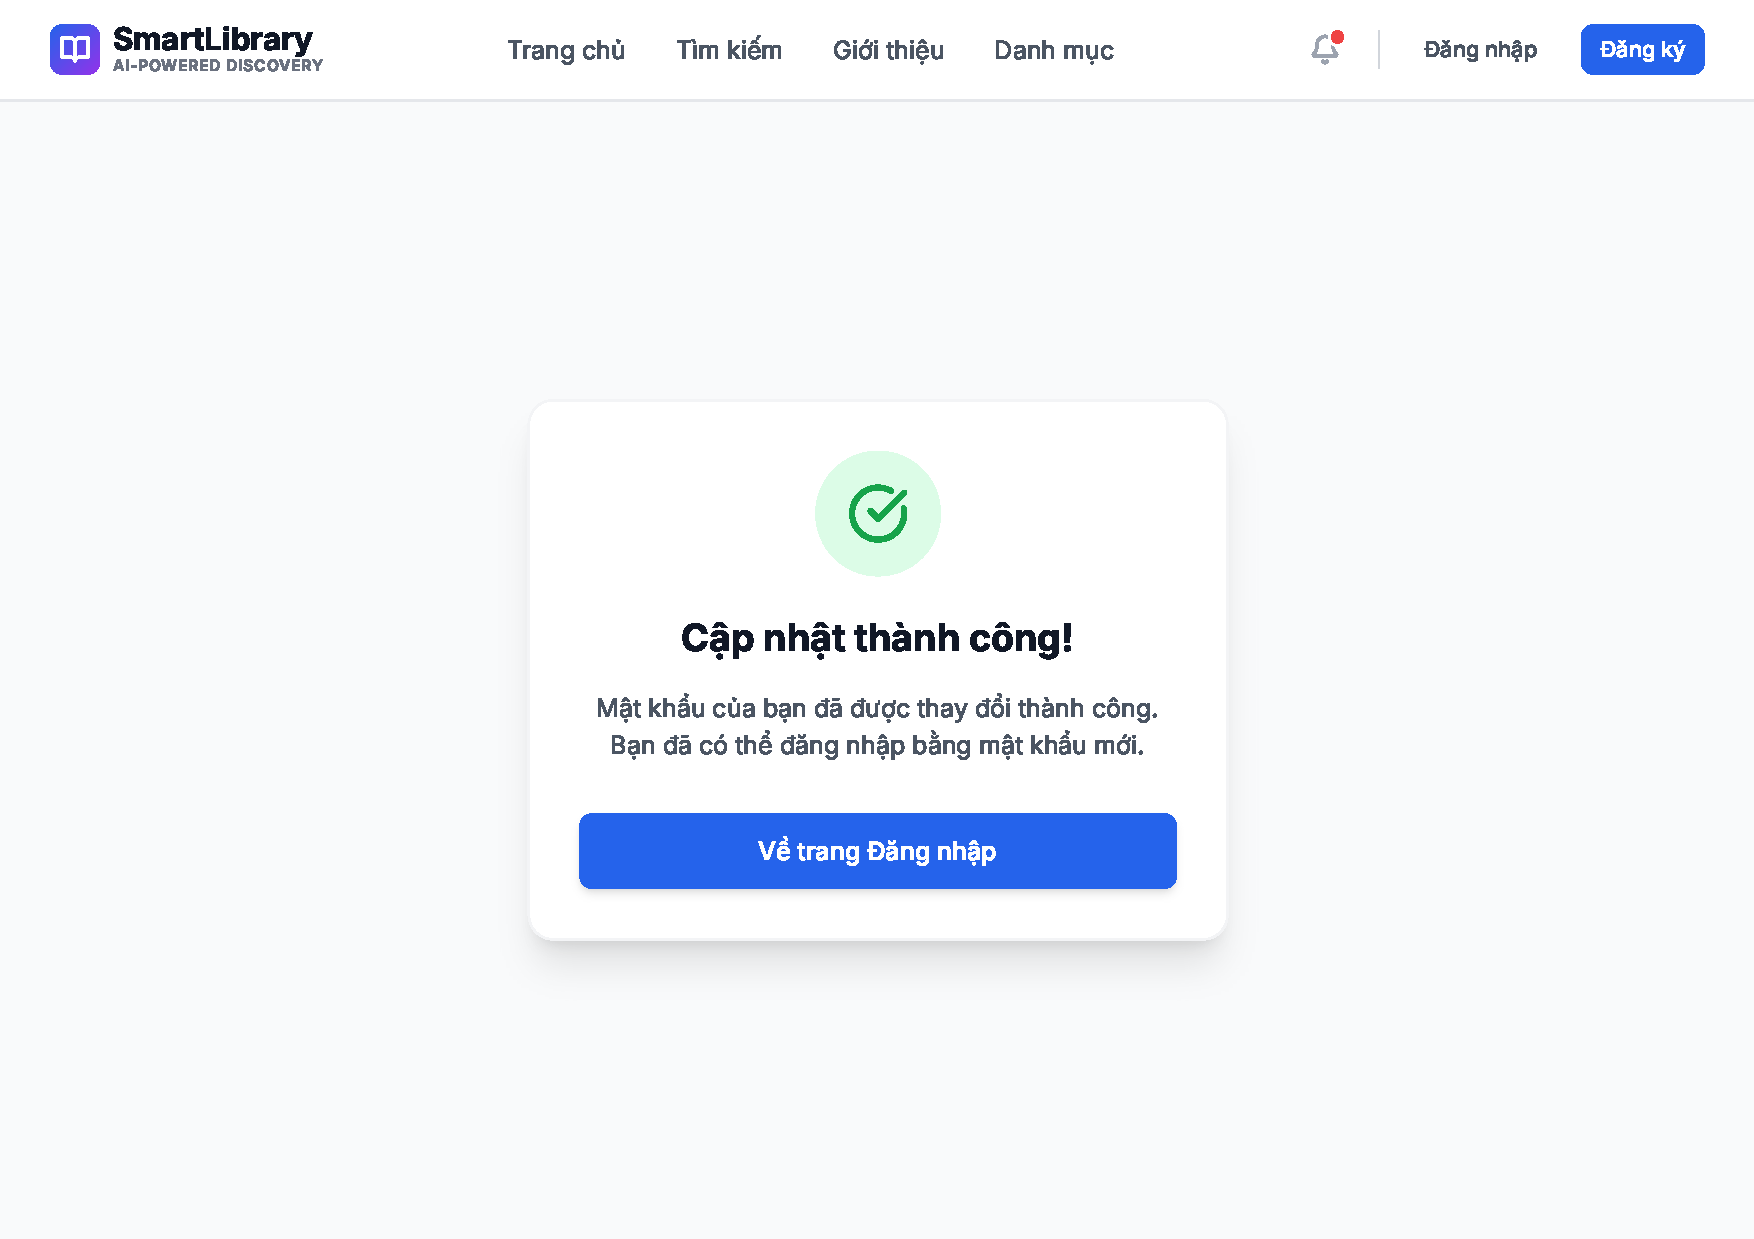
\includegraphics[width=\linewidth]{picture/quenmatkhau/5.pdf}
        \caption{Thông báo cập nhật thành công}
        \label{fig:forgot_pwd_success}
    \end{minipage}
\end{figure}

\noindent\textbf{Mô tả giao diện:} 
Khi truy cập vào đường dẫn hợp lệ, hệ thống sẽ yêu cầu người dùng nhập và xác nhận lại mật khẩu mới. Mật khẩu mới phải đáp ứng tiêu chuẩn bảo mật cơ bản là có độ dài tối thiểu 8 ký tự. Sau khi lưu thông tin, một màn hình thông báo thành công sẽ xuất hiện, xác nhận quá trình thay đổi đã hoàn tất và hỗ trợ người dùng quay lại trang chủ để đăng nhập bằng thông tin vừa tạo.

\vspace{0.5cm}
\subsubsection{Đặc tả luồng nghiệp vụ}

Quy trình khôi phục mật khẩu được thiết kế chặt chẽ thông qua hai giai đoạn tương ứng với hai điểm cuối giao tiếp API như sau:

\noindent\textbf{1. Giai đoạn yêu cầu cấp lại mật khẩu}
\begin{itemize}
    \item \textbf{Endpoint:} \texttt{POST /api/v1/auth/forgot-password}
    \item \textbf{Dữ liệu đầu vào:} Địa chỉ email của người dùng.
    \item \textbf{Logic xử lý:} Máy chủ kiểm tra sự tồn tại của email trong cơ sở dữ liệu. Nếu tài khoản hợp lệ, hệ thống sẽ khởi tạo một mã xác thực bảo mật dạng chuỗi (Token), lưu trữ mã này cùng với hạn sử dụng (30 phút) và kích hoạt dịch vụ gửi thư điện tử. Để tránh việc kẻ gian lợi dụng dò tìm tài khoản, hệ thống luôn trả về thông báo thành công ngay cả khi email không tồn tại.
\end{itemize}

\noindent\textbf{2. Giai đoạn thiết lập mật khẩu mới}
\begin{itemize}
    \item \textbf{Endpoint:} \texttt{POST /api/v1/auth/reset-password}
    \item \textbf{Dữ liệu đầu vào:} Mã xác thực (Token) trích xuất từ đường dẫn và chuỗi Mật khẩu mới.
    \item \textbf{Logic xử lý:} Hệ thống tiến hành xác minh tính hợp lệ và thời hạn của mã xác thực. Nếu mã vượt qua kiểm tra, máy chủ sẽ tiến hành băm (hash) mật khẩu mới để thay thế dữ liệu cũ trong cơ sở dữ liệu, đồng thời vô hiệu hóa ngay lập tức mã xác thực vừa dùng để ngăn chặn việc tái sử dụng.
\end{itemize}
% Preamble cần thiết: \usepackage{graphicx}, \usepackage{float}

\subsection{Thanh điều hướng}

\begin{figure}[H]
    \centering
    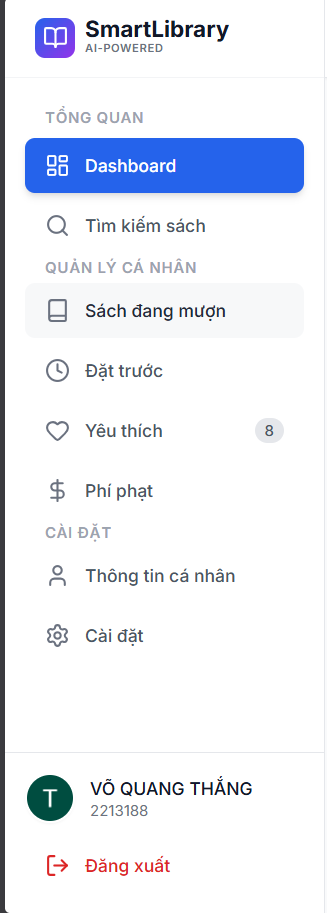
\includegraphics[width=0.35\textwidth]{picture/Sidebar/1.png}
    \caption{Giao diện Thanh điều hướng chính của hệ thống}
    \label{fig:sidebar_menu}
\end{figure}

\noindent\textbf{Mô tả các vùng chức năng:}
\begin{itemize}
    \item \textbf{Khối Tổng quan:} Nơi cung cấp các lối tắt truy cập nhanh vào Bảng điều khiển (Dashboard) và công cụ Tìm kiếm sách.
    \item \textbf{Khối Quản lý cá nhân:} Tập trung các tính năng theo dõi hoạt động của người dùng tại thư viện. Bao gồm quản lý danh sách sách đang mượn, theo dõi tiến trình đặt trước, xem lại danh mục sách yêu thích (hỗ trợ hiển thị trực quan số lượng thông qua huy hiệu đếm) và tra cứu các khoản phí phạt nếu có.
    \item \textbf{Khối Cài đặt \& Tài khoản (Nửa dưới):} Chứa liên kết điều hướng đến trang quản lý hồ sơ cá nhân và thiết lập hệ thống. Điểm nhấn ở cuối thanh điều hướng là thẻ thông tin định danh tĩnh (bao gồm ảnh đại diện, họ tên, mã số sinh viên) giúp người dùng luôn nhận biết được tài khoản đang sử dụng, đi kèm với nút thao tác Đăng xuất nhanh.
\end{itemize}

\vspace{0.5cm}
\noindent\textbf{Logic kỹ thuật cốt lõi:}
\begin{itemize}
    \item \textbf{Cơ chế hiển thị:} Thanh điều hướng được thiết kế tĩnh bên lề trái, áp dụng kiến trúc ứng dụng trang đơn (Single Page Application - SPA) giúp người dùng chuyển đổi mượt mà giữa các phân hệ mà không phải tải lại toàn bộ trang web.
    \item \textbf{Đồng bộ dữ liệu:} Thông tin hiển thị ở thẻ người dùng (tên, mã số) được trích xuất và đồng bộ trực tiếp từ trạng thái lưu trữ của Token (JWT) hiện tại.
    \item \textbf{Xử lý Đăng xuất:} Khi kích hoạt, hệ thống Frontend sẽ tiến hành xóa bỏ toàn bộ Token khỏi bộ nhớ cục bộ (Local Storage/Session) và ngay lập tức điều hướng người dùng quay trở lại màn hình Đăng nhập.
\end{itemize}

\subsection{Quản lý thông tin cá nhân}

\subsubsection{Giao diện Tổng quan hồ sơ}

\begin{figure}[H]
    \centering
    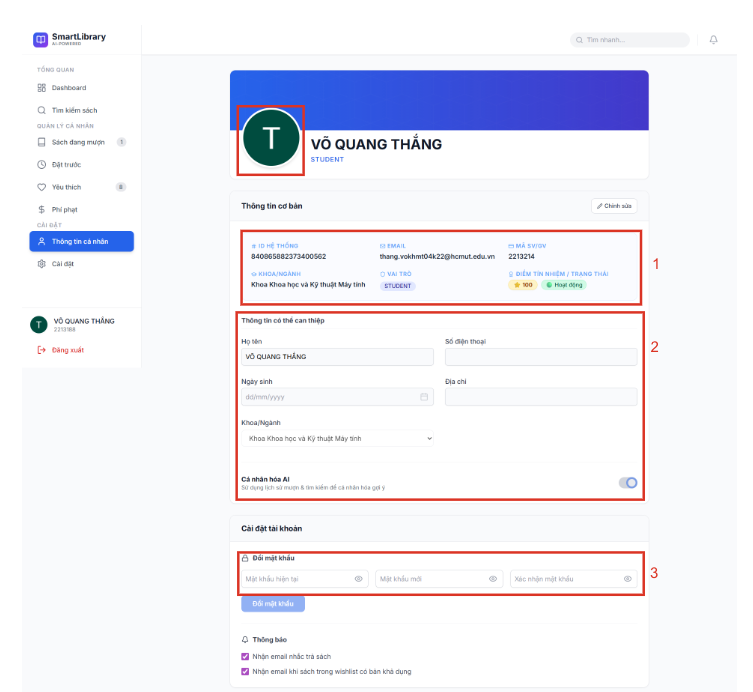
\includegraphics[width=0.9\textwidth]{picture/profile/1.png}
    \caption{Giao diện Quản lý thông tin cá nhân (Profile Dashboard)}
    \label{fig:profile_overview}
\end{figure}

\noindent\textbf{Chú thích các vùng chức năng:}
\begin{itemize}
    \item \textbf{Vùng 1 (Thông tin cơ bản):} Hiển thị các thông tin định danh cốt lõi không thể tự ý thay đổi (chỉ đọc) bao gồm: ID Hệ thống, Email trường, Mã SV/GV, Khoa/Ngành, Vai trò (STUDENT/LIBRARIAN), Điểm tín nhiệm (mặc định 100) và Trạng thái hoạt động.
    \item \textbf{Vùng 2 (Thông tin có thể can thiệp):} Biểu mẫu cho phép người dùng tự cập nhật các thông tin cá nhân như: Họ tên, Số điện thoại, Ngày sinh, Địa chỉ. Ngoài ra còn có công tắc bật/tắt tính năng "Cá nhân hóa AI" (sử dụng lịch sử mượn để AI gợi ý sách).
    \item \textbf{Vùng 3 (Cài đặt tài khoản):} Khu vực hỗ trợ bảo mật và tùy chọn hệ thống, bao gồm biểu mẫu đổi mật khẩu (yêu cầu mật khẩu hiện tại) và các tùy chọn nhận thông báo qua email.
\end{itemize}

\subsubsection{Giao diện Cập nhật ảnh đại diện}

\begin{figure}[H]
    \centering
    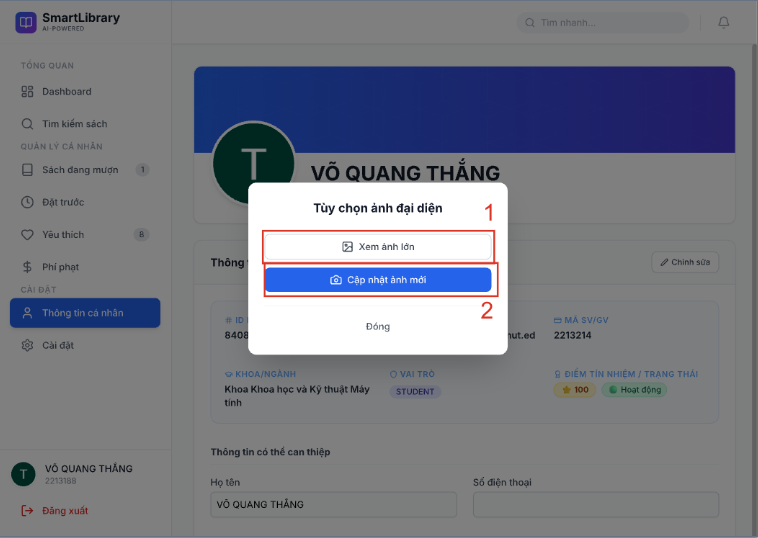
\includegraphics[width=0.8\textwidth]{picture/profile/2.png}
    \caption{Menu tùy chọn thao tác với ảnh đại diện}
    \label{fig:profile_avatar_menu}
\end{figure}

\noindent\textbf{Chú thích giao diện (Hình \ref{fig:profile_avatar_menu}):} Khi người dùng tương tác (click) vào ảnh đại diện hiện tại, hệ thống hiển thị một menu với hai lựa chọn:
\begin{itemize}
    \item \textbf{Vùng 1 (Xem ảnh lớn):} Phóng to ảnh đại diện hiện tại.
    \item \textbf{Vùng 2 (Cập nhật ảnh mới):} Kích hoạt luồng tải lên ảnh đại diện mới từ thiết bị cá nhân.
\end{itemize}

\begin{figure}[H]
    \centering
    \begin{minipage}{0.48\textwidth}
        \centering
        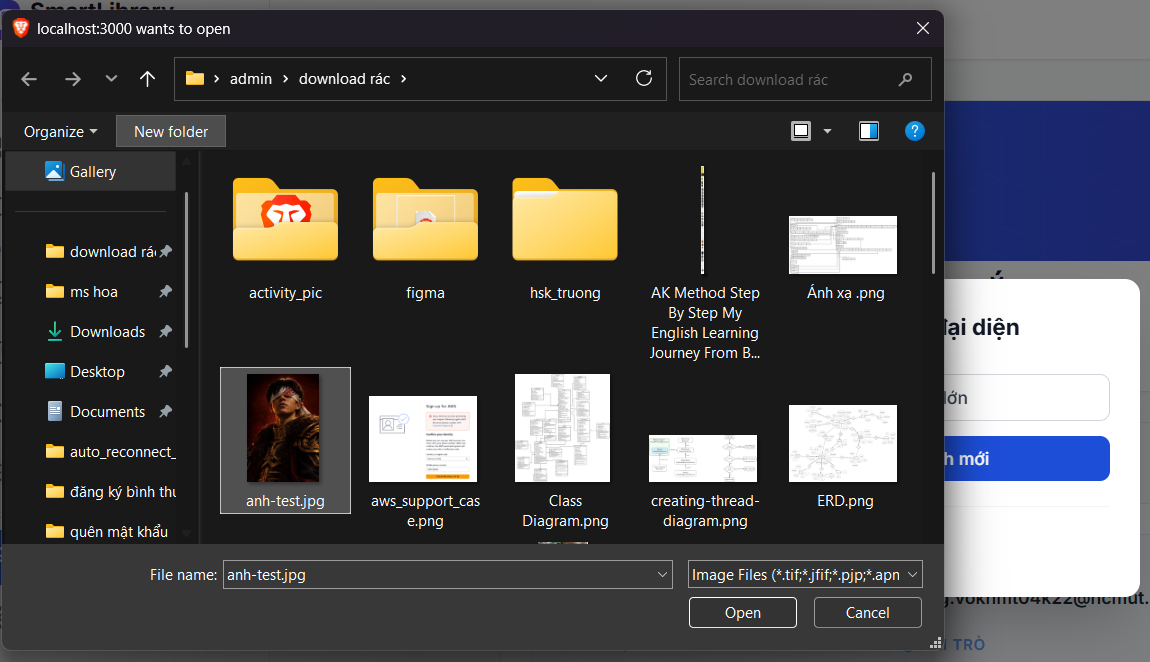
\includegraphics[width=\linewidth]{picture/profile/3.png}
        \caption{Hộp thoại chọn tệp tin}
        \label{fig:profile_file_picker}
    \end{minipage}\hfill
    \begin{minipage}{0.48\textwidth}
        \centering
        
\includegraphics[width=\linewidth]{picture/profile/4.png}
        \caption{Ảnh đại diện sau khi cập nhật}
        \label{fig:profile_avatar_updated}
    \end{minipage}
\end{figure}

\noindent\textbf{Mô tả nghiệp vụ cập nhật ảnh:} Khi chọn "Cập nhật ảnh mới", hệ thống gọi hộp thoại chọn tệp của hệ điều hành (Hình \ref{fig:profile_file_picker}). File ảnh sau khi chọn sẽ được mã hóa dạng \texttt{multipart/form-data} và đẩy lên máy chủ. Giao diện sau đó tự động cập nhật hình ảnh hiển thị mới ngay lập tức mà không cần tải lại trang (Hình \ref{fig:profile_avatar_updated}).

\vspace{0.5cm}
\subsubsection{Đặc tả API và Kỹ thuật}

Tất cả các API trong phân hệ quản lý hồ sơ cá nhân đều yêu cầu xác thực bảo mật bằng JWT. Hệ thống tự động trích xuất mã định danh người dùng (\texttt{userId}) từ JWT token thông qua \texttt{SecurityEvaluator}, tuyệt đối không nhận \texttt{userId} truyền từ phía client để tránh rủi ro bảo mật. Base endpoint cho phân hệ này là \texttt{/api/v1/users}.

\begin{table}[H]
    \centering
    \caption{Danh sách các API phân hệ Thông tin cá nhân}
    \renewcommand{\arraystretch}{1.3}
    \begin{tabularx}{\textwidth}{|l|l|X|}
        \hline
        \textbf{Method} & \textbf{Endpoint} & \textbf{Mô tả nghiệp vụ} \\ \hline
        GET & \texttt{/my-profile} & Lấy toàn bộ thông tin cá nhân của người dùng đang đăng nhập để hiển thị lên giao diện. \\ \hline
        PUT & \texttt{/my-profile} & Cập nhật thông tin (Họ tên, ngày sinh, sđt, địa chỉ). \\ \hline
        POST & \texttt{/avatar} & Tải lên ảnh đại diện mới (\texttt{multipart/form-data}). \\ \hline
        PUT & \texttt{/my-profile/change-password} & Đổi mật khẩu tài khoản. \\ \hline
    \end{tabularx}
\end{table}

\noindent\textbf{Ràng buộc dữ liệu tại Backend:}
\begin{itemize}
    \item \textbf{fullName):} Giới hạn \texttt{@Pattern} (chỉ chứa chữ cái và khoảng trắng).
    \item \textbf{phoneNumber :} Giới hạn \texttt{@Pattern} (từ 10 đến 15 chữ số).
    \item \textbf{dateOfBirth :} Ràng buộc \texttt{@Past} (ngày sinh phải nằm trong quá khứ).
    \item \textbf{address :} Giới hạn \texttt{@Size} (tối đa 200 ký tự).
\end{itemize}

\noindent\textbf{Luồng xử lý Upload Ảnh đại diện (Avatar):}
Máy chủ Backend tiếp nhận file qua định dạng \texttt{multipart/form-data}, sau đó trực tiếp đẩy file lưu trữ lên dịch vụ điện toán đám mây Amazon S3 theo đường dẫn \texttt{avatars/\{userId\}}. Dịch vụ S3 sẽ trả về một đường dẫn (URL) lưu trữ tĩnh. Backend lưu URL này vào cơ sở dữ liệu (\texttt{profilePictureUrl}) và trả URL về cho Frontend để cập nhật giao diện.

\noindent\textbf{Luồng xử lý Đổi mật khẩu:}
Người dùng nhập 3 trường: mật khẩu hiện tại, mật khẩu mới, và xác nhận mật khẩu mới. Tại Frontend, hệ thống xác thực mật khẩu mới không rỗng và khớp với trường xác nhận. Tại Backend, máy chủ đối chiếu mật khẩu hiện tại trong cơ sở dữ liệu. Nếu chính xác, hệ thống tiến hành băm (hash) mật khẩu mới và lưu lại.
% Preamble cần thiết: \usepackage{graphicx}, \usepackage{float}, \usepackage{tabularx}, \usepackage{booktabs}

\subsection{Bảng điều khiển Độc giả}

\subsubsection{Giao diện Tổng quan}

\begin{figure}[H]
    \centering
    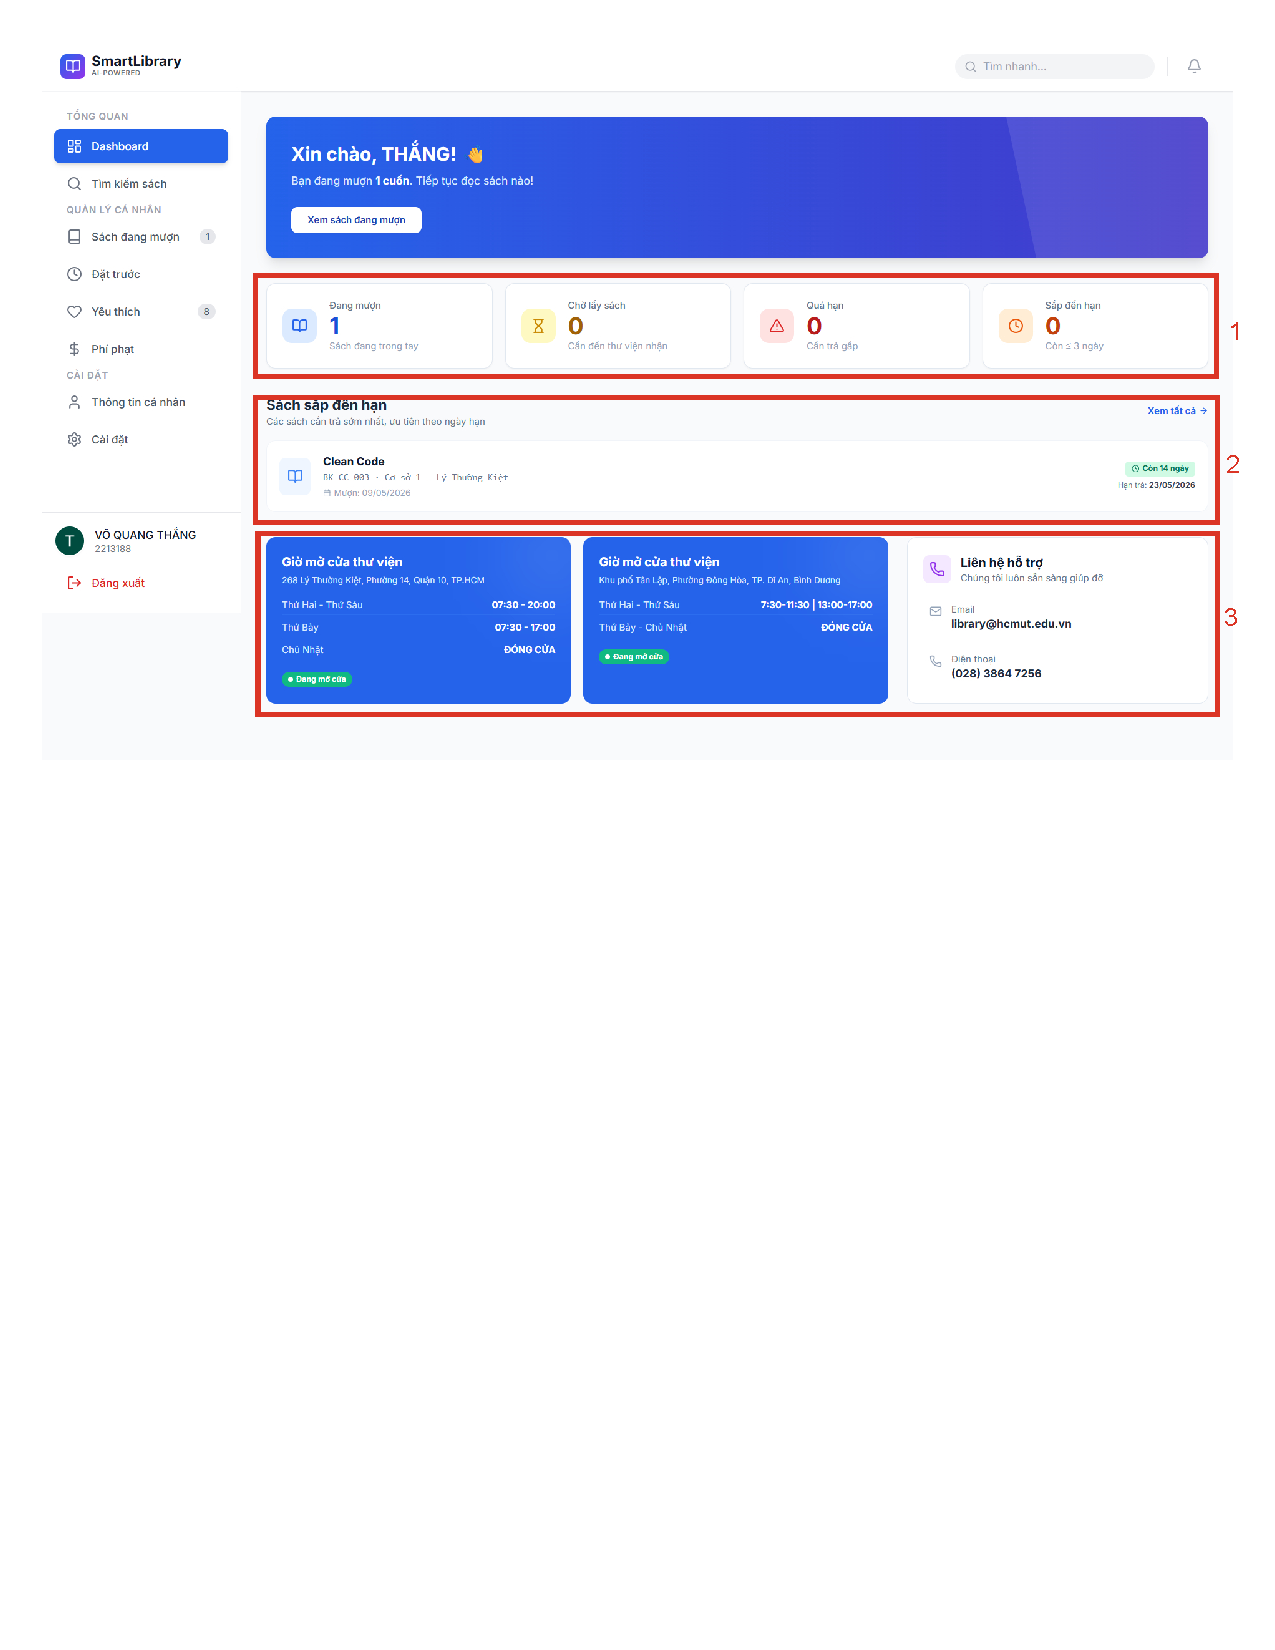
\includegraphics[width=\textwidth]{picture/dashboarddocgia/1.pdf}
    \caption{Giao diện Bảng điều khiển dành cho Sinh viên/Độc giả}
    \label{fig:reader_dashboard}
\end{figure}

\noindent\textbf{Chú thích các vùng chức năng:}
\begin{itemize}
    \item \textbf{Khối Lời chào (Phía trên cùng):} Lời chào được cá nhân hóa dựa trên tên của người dùng đang đăng nhập. Khu vực này cũng cung cấp một thông điệp tóm tắt nhanh (ví dụ: "Bạn đang mượn 1 cuốn") kèm theo nút điều hướng trực tiếp đến danh sách sách đang mượn để độc giả tiện theo dõi.
    
    \item \textbf{Vùng 1 (Thống kê hoạt động cá nhân):} Hiển thị các chỉ số cốt lõi về tình trạng giao dịch hiện tại của độc giả thông qua 4 thẻ (card) trực quan:
    \begin{itemize}
        \item \textit{Đang mượn:} Số lượng sách thực tế đang được giữ bởi độc giả.
        \item \textit{Chờ lấy sách:} Số lượng yêu cầu đặt trước đã được thư viện chuẩn bị xong và đang chờ người dùng đến nhận.
        \item \textit{Quá hạn:} Cảnh báo đỏ về số lượng sách đã vượt quá thời hạn hoàn trả, yêu cầu độc giả xử lý gấp để tránh phát sinh thêm phí phạt.
        \item \textit{Sắp đến hạn:} Số sách chuẩn bị đến hạn trả trong một vài ngày tới.
    \end{itemize}
    
    \item \textbf{Vùng 2 (Danh sách sách sắp đến hạn):} Khu vực cảnh báo chi tiết, liệt kê cụ thể những cuốn sách mà người dùng cần trả sớm. Thông tin hiển thị bao gồm tiêu đề sách, vị trí cơ sở mượn (ví dụ: Cơ sở Lý Thường Kiệt), số ngày còn lại và mốc thời gian hoàn trả chính xác. Mục này giúp độc giả chủ động sắp xếp thời gian đến thư viện.
    
    \item \textbf{Vùng 3 (Thông tin vận hành thư viện):} Bảng thông tin tĩnh cung cấp lịch hoạt động của cả hai cơ sở thư viện (Cơ sở Lý Thường Kiệt và Cơ sở Dĩ An). Tùy thuộc vào thời gian thực của hệ thống, giao diện sẽ tự động hiển thị nhãn "Đang mở cửa" (màu xanh) hoặc "Đóng cửa" để hỗ trợ độc giả lên kế hoạch di chuyển. Bên cạnh đó là các kênh liên hệ đường dây nóng và email hỗ trợ của nhà trường.
\end{itemize}

\vspace{0.5cm}
\subsubsection{Đặc tả luồng nghiệp vụ Bảng điều khiển}

Bảng điều khiển của độc giả đóng vai trò là trạm thông tin trung tâm. Để tải toàn bộ dữ liệu cho màn hình này, hệ thống Frontend sẽ gọi song song các API để tối ưu hóa thời gian tải trang.

\noindent\textbf{1. Truy xuất thống kê giao dịch}
\begin{itemize}
    \item \textbf{Endpoint:} \texttt{GET /api/v1/transactions/me/summary} (hoặc tập hợp các lệnh đếm từ API giao dịch cá nhân).
    \item \textbf{Quyền truy cập:} STUDENT / LECTURER.
    \item \textbf{Logic xử lý:} Máy chủ truy vấn cơ sở dữ liệu dựa trên \texttt{userId} của người dùng hiện tại, tính toán và gom nhóm (GROUP BY) số lượng giao dịch theo các trạng thái: Đang mượn (\texttt{BORROWED}), Chờ lấy (\texttt{RESERVED}), Quá hạn (\texttt{OVERDUE}) và Sắp đến hạn (các giao dịch \texttt{BORROWED} có \texttt{dueDate} nhỏ hơn 3 ngày tới).
\end{itemize}

\noindent\textbf{2. Truy xuất danh sách cần chú ý (Sắp đến hạn)}
\begin{itemize}
    \item \textbf{Endpoint:} \texttt{GET /api/v1/transactions/me?status=BORROWED\&sort=dueDate,asc\&size=5}
    \item \textbf{Logic xử lý:} Hệ thống trả về danh sách tối đa 5 giao dịch đang mượn, được sắp xếp ưu tiên theo ngày hạn trả tăng dần (những cuốn sắp đến hạn nhất sẽ nằm trên cùng) để hiển thị ra Vùng 2 của giao diện.
\end{itemize}

% Preamble cần thiết: \usepackage{graphicx}, \usepackage{float}, \usepackage{tabularx}, \usepackage{booktabs}

\subsection{Khám phá và Tìm kiếm tài liệu}

\subsubsection{Giao diện Tìm kiếm tổng hợp}

\begin{figure}[H]
    \centering
    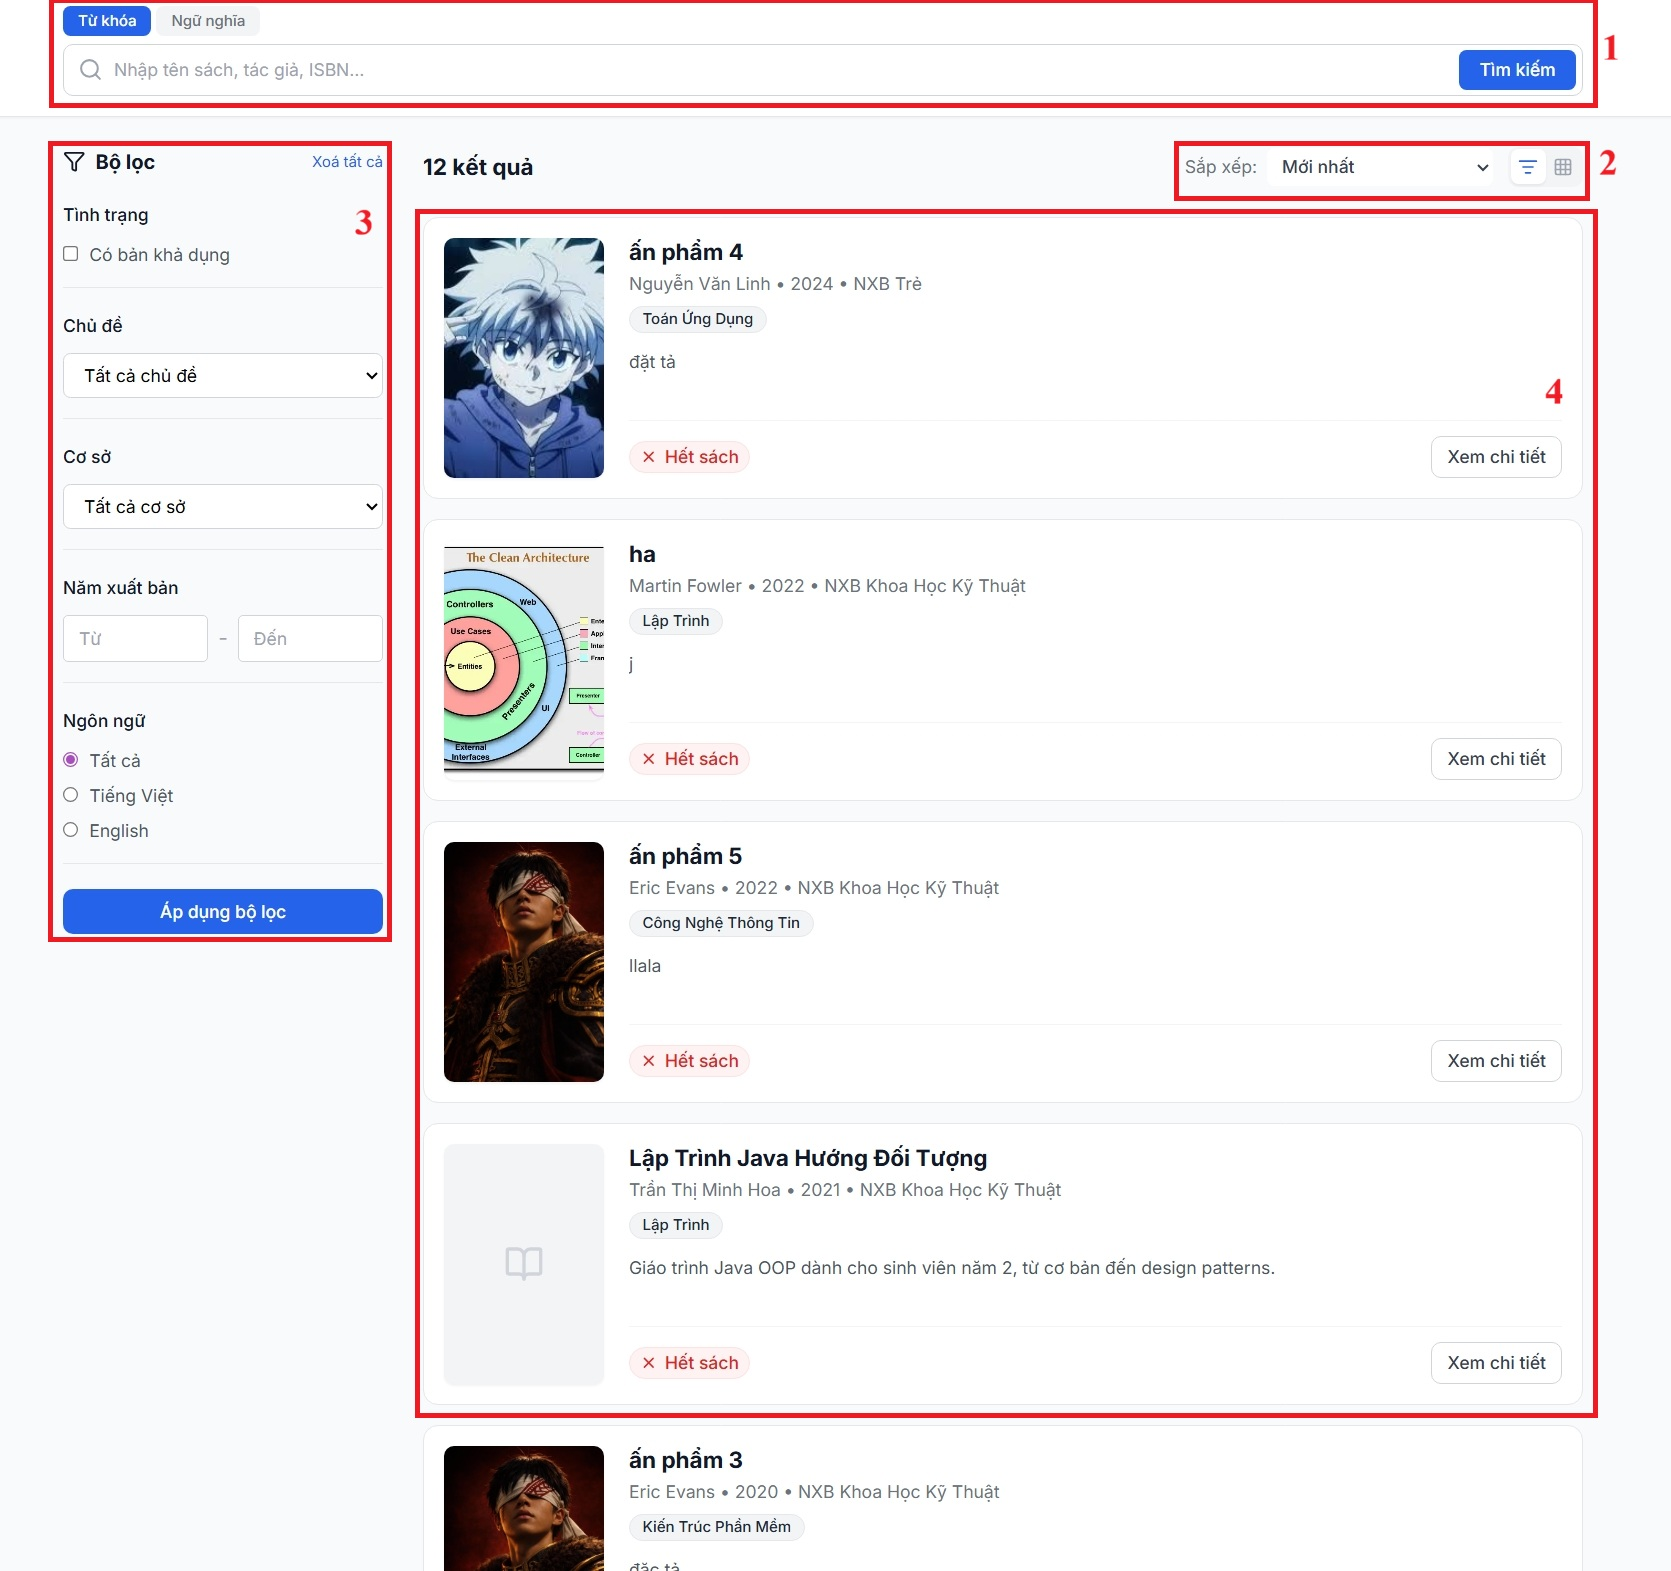
\includegraphics[width=\textwidth]{picture/publictimkiemchitiet/1timkiem.jpeg}
    \caption{Giao diện Tìm kiếm và Bộ lọc nâng cao}
    \label{fig:public_search}
\end{figure}

\noindent\textbf{Chú thích các vùng chức năng:}
\begin{itemize}
    \item \textbf{Vùng 1 (Thanh tìm kiếm trung tâm):} Khu vực nhập từ khóa tự do. Khung tìm kiếm hỗ trợ tra cứu linh hoạt qua nhiều tiêu chí như tên sách, tên tác giả, hoặc mã số chuẩn quốc tế (ISBN).
    \item \textbf{Vùng 2 (Công cụ hiển thị):} Thanh công cụ hỗ trợ người dùng sắp xếp kết quả (theo độ mới, lượt mượn, đánh giá) và linh hoạt chuyển đổi chế độ xem giữa dạng danh sách (List) hoặc dạng lưới (Grid).
    \item \textbf{Vùng 3 (Bộ lọc đa chiều):} Hệ thống cung cấp các bộ lọc sâu để thu hẹp kết quả, bao gồm: tình trạng (chỉ hiện sách còn bản sao khả dụng), chủ đề chuyên ngành, cơ sở lưu trữ (Lý Thường Kiệt hoặc Dĩ An), khoảng thời gian xuất bản và ngôn ngữ.
    \item \textbf{Vùng 4 (Danh sách kết quả):} Khu vực trình bày các ấn phẩm thỏa mãn tiêu chí tìm kiếm. Mỗi thẻ ấn phẩm hiển thị ảnh bìa, tiêu đề, tác giả, năm xuất bản và nhãn trạng thái (ví dụ: "Hết sách" khi toàn bộ bản sao đang được mượn).
\end{itemize}

\vspace{0.5cm}
\noindent\textbf{Đặc tả luồng nghiệp vụ Tìm kiếm:}
\begin{itemize}
    \item \textbf{Điểm cuối (Endpoint):} \texttt{GET /api/v1/publications/search}
    \item \textbf{Quyền truy cập:} Công khai (Không yêu cầu đăng nhập).
    \item \textbf{Chiến lược truy vấn (SQL Strategy):} Để tối ưu hóa hiệu suất tìm kiếm linh hoạt mà không cần đến các engine bên ngoài như Elasticsearch, máy chủ Backend sử dụng \texttt{NamedParameterJdbcTemplate}. Truy vấn tìm kiếm từ khóa (\texttt{keyword}) được thực thi theo dạng không phân biệt hoa thường (\texttt{ILIKE}) quét qua 6 bảng dữ liệu liên kết: bảng Tiêu đề sách, Tiêu đề phụ, Mã ISBN, bảng Tác giả, bảng Từ khóa (Tags) và bảng Thể loại.
    \item \textbf{Logic Sắp xếp (Sorting):} Nếu người dùng tìm theo từ khóa, kết quả được sắp xếp theo độ liên quan (mức độ khớp của tiêu đề được ưu tiên cao nhất). Nếu sắp xếp theo "Lượt mượn nhiều nhất", hệ thống sử dụng truy vấn con đếm tổng số giao dịch mượn. Nếu sắp xếp theo "Đánh giá", hệ thống dựa vào điểm đánh giá trung bình.
\end{itemize}

\subsubsection{Giao diện Chi tiết ấn phẩm}

Khi người dùng chọn một ấn phẩm từ kết quả tìm kiếm, hệ thống sẽ điều hướng sang trang Chi tiết ấn phẩm. Màn hình này được chia thành nhiều khối thông tin chuyên sâu.

\begin{figure}[H]
    \centering
    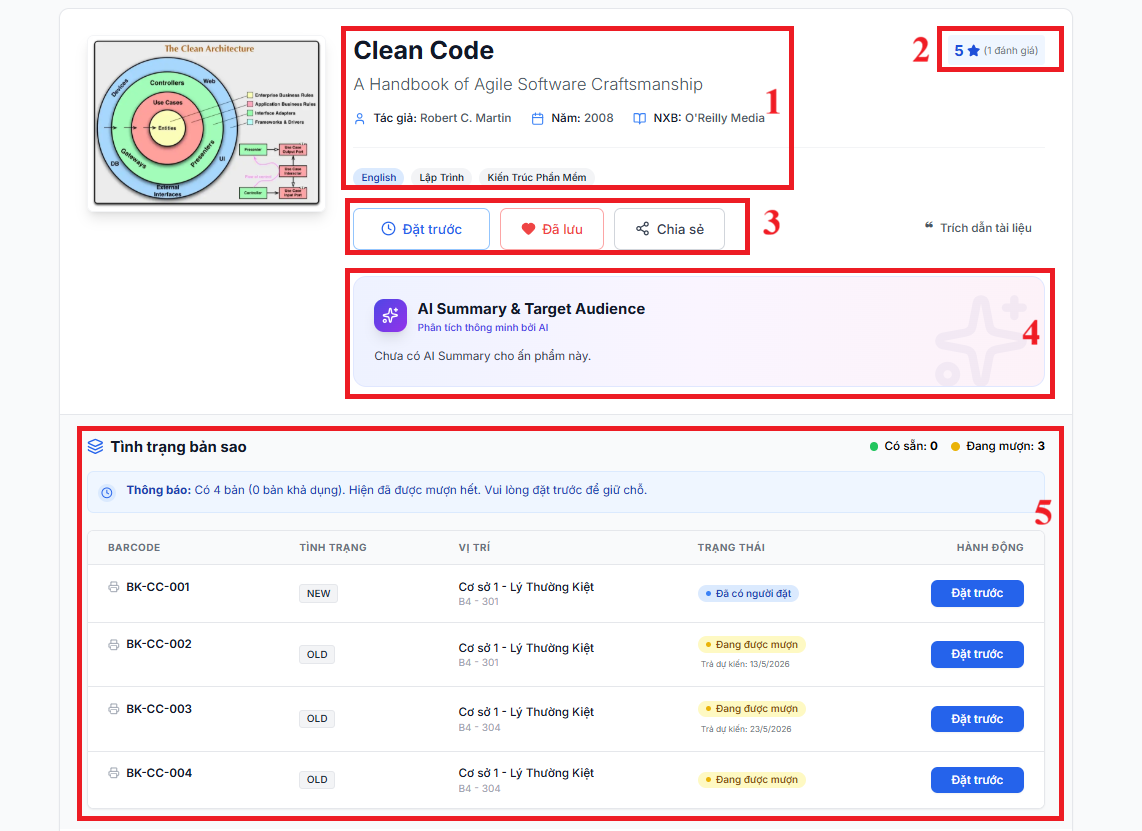
\includegraphics[width=\textwidth]{picture/publictimkiemchitiet/2chitietsach.png}
    \caption{Giao diện Thông tin tổng quan và Tình trạng mượn trả}
    \label{fig:public_detail_top}
\end{figure}

\noindent\textbf{Chú thích giao diện (Hình \ref{fig:public_detail_top}):}
\begin{itemize}
    \item \textbf{Vùng 1 (Thông tin nền tảng):} Hiển thị ảnh bìa, nhan đề chính, nhan đề phụ, tác giả, năm và nhà xuất bản, kèm theo các thẻ phân loại (Tags).
    \item \textbf{Vùng 2 (Chỉ số đánh giá):} Điểm số trung bình dựa trên phản hồi của độc giả hệ thống.
    \item \textbf{Vùng 3 (Thanh thao tác):} Các hành động người dùng có thể thực hiện bao gồm Đặt trước sách, Lưu vào danh sách yêu thích và Lấy liên kết chia sẻ.
    \item \textbf{Vùng 4 (Phân tích Trí tuệ nhân tạo):} Khu vực đặc biệt tích hợp AI nhằm tự động tóm tắt nội dung sách và đề xuất tệp độc giả mục tiêu phù hợp.
    \item \textbf{Vùng 5 (Tình trạng bản sao vật lý):} Danh sách thời gian thực các quyển sách vật lý đang tồn tại trong thư viện. Bảng này cung cấp mã vạch, tình trạng sách (Mới/Cũ), vị trí kệ, trạng thái (Có sẵn/Đang mượn) và nút hành động tương ứng. Nếu một bản sao đang được mượn, hệ thống sẽ dự báo ngày có thể trả lại.
\end{itemize}

\begin{figure}[H]
    \centering
    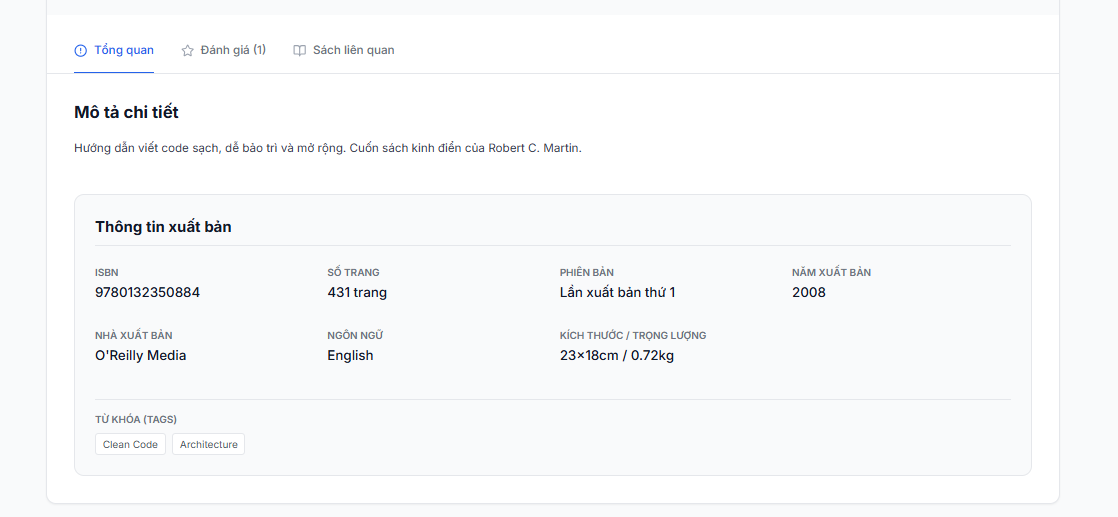
\includegraphics[width=0.85\textwidth]{picture/publictimkiemchitiet/3metadatachitiet.png}
    \caption{Khối dữ liệu Mô tả nội dung và Thông số xuất bản}
    \label{fig:public_detail_bottom}
\end{figure}

\noindent\textbf{Chú thích giao diện (Hình \ref{fig:public_detail_bottom}):} Khu vực tab mở rộng cung cấp đoạn văn mô tả chi tiết nội dung sách và một bảng ma trận các thông số kỹ thuật xuất bản (Mã ISBN, Số trang, Phiên bản, Kích thước vật lý, Trọng lượng).

\vspace{0.5cm}
\noindent\textbf{Đặc tả luồng nghiệp vụ Chi tiết ấn phẩm:}

Trang chi tiết yêu cầu một khối lượng dữ liệu khổng lồ từ nhiều phân hệ khác nhau. Để tải trang nhanh chóng, hệ thống sử dụng cơ chế chia nhỏ truy vấn thông qua hai API song song.

\noindent\textbf{1. Truy xuất thông tin metadata ấn phẩm}
\begin{itemize}
    \item \textbf{Điểm cuối:} \texttt{GET /api/v1/publications/\{id\}}
    \item \textbf{Logic xử lý dữ liệu:} Thay vì sử dụng một truy vấn kết nối (JOIN) khổng lồ dễ gây thắt cổ chai, Backend được thiết kế thực thi 6 truy vấn độc lập (Lấy thông tin gốc; Lấy danh sách Tác giả; Lấy bộ Từ khóa; Lấy Danh mục; Tính trung bình Đánh giá; Thống kê số lượng sách). Kết quả từ 6 luồng này được máy chủ tổng hợp (Aggregate) lại thành một gói phản hồi duy nhất gửi về Frontend.
\end{itemize}

\noindent\textbf{2. Truy xuất tình trạng bản sao vật lý (Vùng 5)}
\begin{itemize}
    \item \textbf{Điểm cuối:} \texttt{GET /api/v1/publications/\{id\}/items}
    \item \textbf{Logic xử lý dữ liệu:} API này trả về danh sách các quyển sách vật lý phục vụ cho việc đặt trước. Backend sử dụng ngôn ngữ truy vấn JPQL thực hiện phép kết nối trái (LEFT JOIN) với bảng Lịch sử Giao dịch. Kỹ thuật này giúp hệ thống tìm ra mức ngày hạn trả lớn nhất (\texttt{MAX(dueDate)}) của các giao dịch đang diễn ra (\texttt{status = 'BORROWING'}), từ đó tính toán và hiển thị chính xác ngày dự kiến sách được trả về kho cho độc giả.
\end{itemize}

% Preamble cần thiết: \usepackage{graphicx}, \usepackage{float}, \usepackage{tabularx}, \usepackage{booktabs}

\subsection{Danh sách sách yêu thích và Thông báo}

\subsubsection{Giao diện quản lý danh sách yêu thích}

\begin{figure}[H]
    \centering
    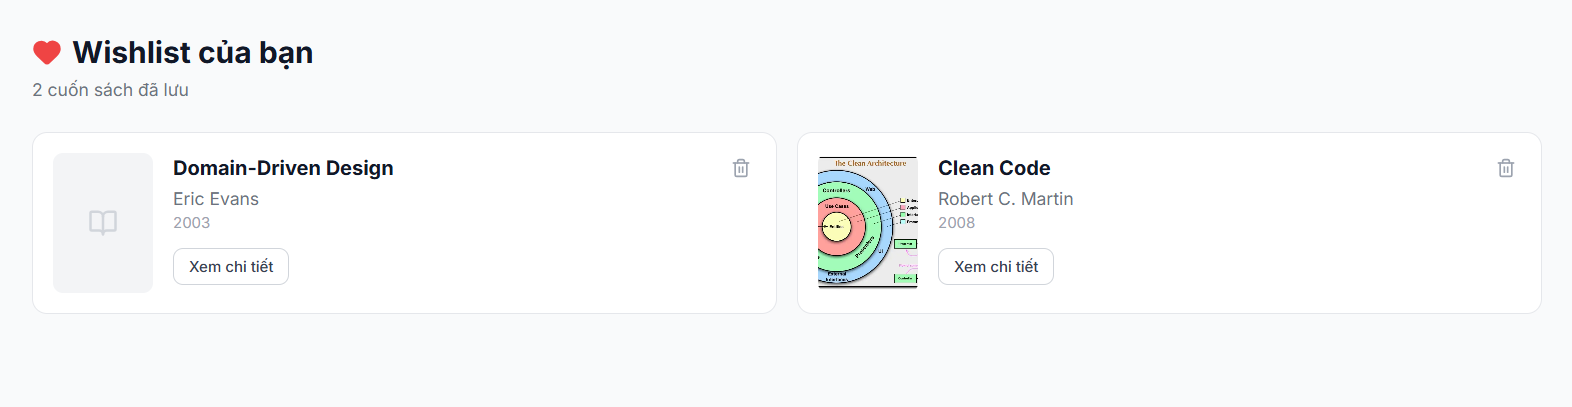
\includegraphics[width=\textwidth]{picture/wishlist/1danhsachwishlist.png}
    \caption{Giao diện quản lý danh sách sách đã lưu của độc giả}
    \label{fig:wishlist_list}
\end{figure}

\noindent\textbf{Chú thích giao diện:} 
Trang quản lý danh sách yêu thích được trình bày dưới dạng lưới trực quan. Mỗi thẻ thông tin sách cung cấp đầy đủ ảnh bìa, tiêu đề, tên tác giả và năm xuất bản. Từ đây, độc giả có thể dùng nút "Xem chi tiết" để chuyển hướng nhanh đến trang thông tin của ấn phẩm, hoặc nhấn vào biểu tượng thùng rác để gỡ bỏ sách khỏi danh sách lưu trữ.

\begin{figure}[H]
    \centering
    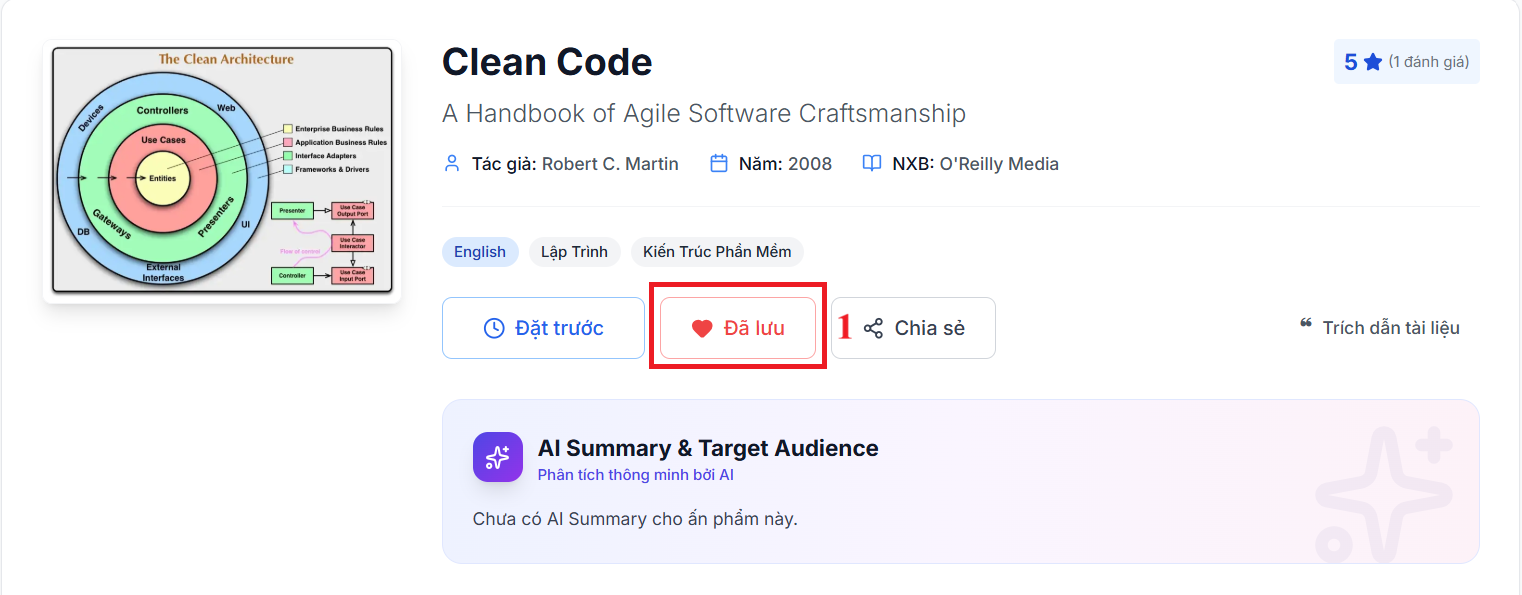
\includegraphics[width=\textwidth]{picture/wishlist/2iconwishlist.png}
    \caption{Nút thao tác lưu sách tại trang chi tiết ấn phẩm}
    \label{fig:wishlist_icon}
\end{figure}

\noindent\textbf{Chú thích giao diện:} 
Tại trang chi tiết của mỗi ấn phẩm, hệ thống bố trí một nút thao tác lưu sách nổi bật. Trạng thái của nút này (đã lưu hoặc chưa lưu) được hệ thống đánh giá và hiển thị theo thời gian thực dựa trên dữ liệu cá nhân hóa của từng người dùng.

\vspace{0.5cm}
\subsubsection{Đặc tả API và Luồng xử lý dữ liệu}

Hệ thống cung cấp một nhóm giao tiếp (API) chuyên trách cho tính năng lưu sách với đường dẫn gốc là \texttt{/api/v1/wishlist}. Để đảm bảo bảo mật, toàn bộ các điểm cuối đều yêu cầu người dùng phải xác thực hệ thống (Authentication) trước khi sử dụng.

\begin{table}[H]
    \centering
    \caption{Danh sách API Quản lý sách yêu thích}
    \renewcommand{\arraystretch}{1.3}
    \begin{tabularx}{\textwidth}{|l|l|X|}
        \hline
        \textbf{Phương thức} & \textbf{Điểm cuối} & \textbf{Mô tả nghiệp vụ} \\ \hline
        GET & \texttt{/} & Truy xuất toàn bộ danh sách sách đã lưu của người dùng hiện tại. \\ \hline
        POST & \texttt{/\{publicationId\}} & Thêm một ấn phẩm mới vào danh sách yêu thích. \\ \hline
        DELETE & \texttt{/\{publicationId\}} & Gỡ bỏ một ấn phẩm ra khỏi danh sách. \\ \hline
        GET & \texttt{/\{publicationId\}/status} & Kiểm tra trạng thái lưu của một ấn phẩm cụ thể. \\ \hline
    \end{tabularx}
\end{table}

\noindent\textbf{Logic nghiệp vụ cốt lõi:}
\begin{itemize}
    \item \textbf{Thao tác thêm sách:} Khi nhận yêu cầu, hệ thống sẽ kiểm tra danh sách của người dùng và tự động tạo mới nếu chưa có. Điểm đặc biệt của quy trình này là tính độc lập (Idempotent): nếu sách đã tồn tại trong danh sách, hệ thống vẫn ghi nhận thành công mà không phát sinh lỗi. Đồng thời, mỗi lượt lưu sách sẽ ngầm tạo ra một bản ghi tương tác để cung cấp dữ liệu huấn luyện cho hệ thống Trí tuệ Nhân tạo (AI) gợi ý sách sau này.
    \item \textbf{Thao tác gỡ bỏ:} Khi người dùng yêu cầu xóa, hệ thống tiến hành gỡ bỏ ấn phẩm và trả về kết quả. Giao diện chỉ làm mới danh sách và hiển thị thông báo thành công sau khi nhận được phản hồi chính thức từ máy chủ (hệ thống không sử dụng kỹ thuật cập nhật lạc quan - Optimistic Update nhằm đảm bảo tính đồng nhất dữ liệu).
    \item \textbf{Truy xuất dữ liệu:} Thông tin trả về được tối ưu hóa hiệu suất bằng các truy vấn cơ sở dữ liệu nguyên thủy (Native SQL). Dữ liệu tác giả được gom nhóm gọn gàng thông qua hàm \texttt{STRING\_AGG}. Danh sách trả về luôn được sắp xếp theo thời gian ưu tiên những cuốn sách mới được thêm vào gần nhất.
\end{itemize}

\subsubsection{Hệ thống thông báo và nhắc nhở mượn sách}

\begin{figure}[H]
    \centering
    \begin{minipage}{0.48\textwidth}
        \centering
        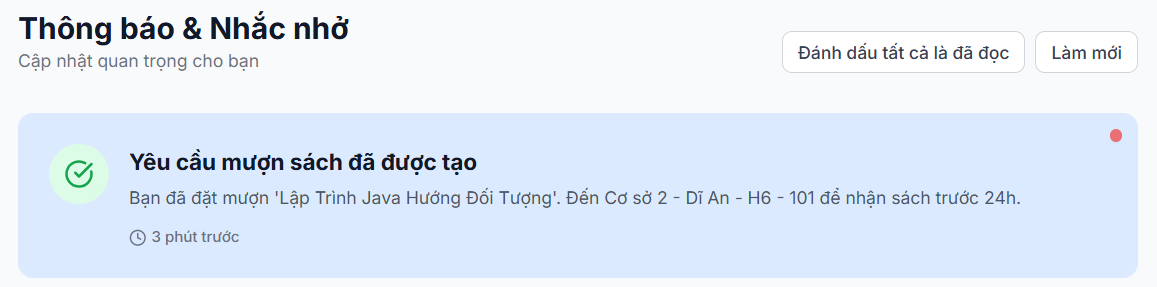
\includegraphics[width=\linewidth]{picture/wishlist/4thongbaoveviecdanhacnholaysachtruoc24h.png}
        \caption{Thông báo đẩy trên hệ thống web}
        \label{fig:wishlist_noti_web}
    \end{minipage}\hfill
    \begin{minipage}{0.48\textwidth}
        \centering
        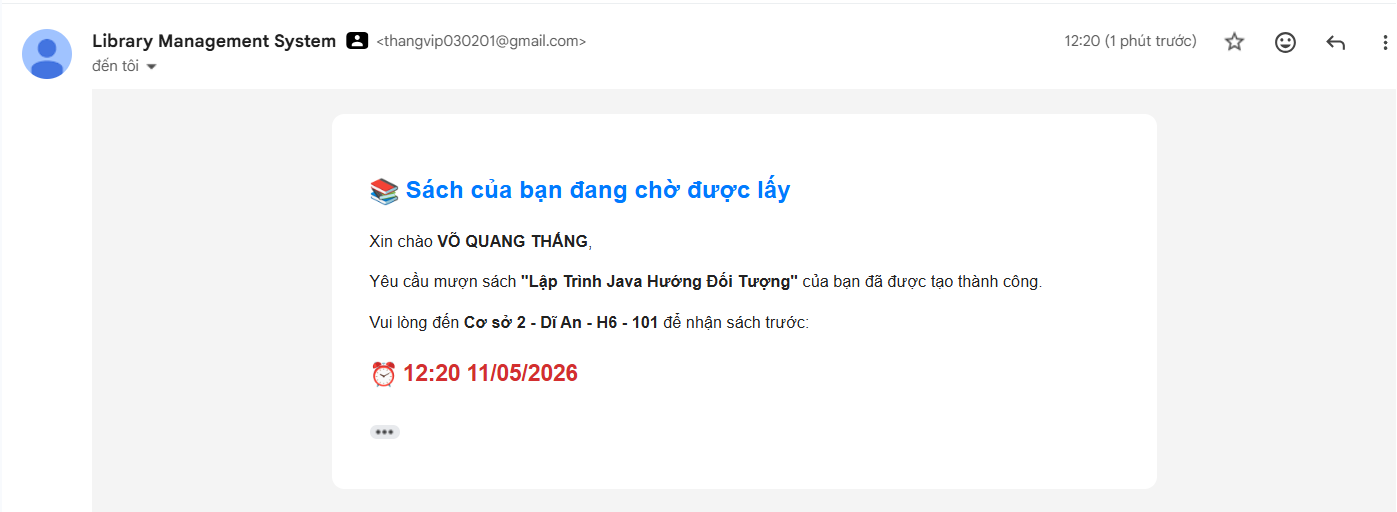
\includegraphics[width=\linewidth]{picture/wishlist/3emailnhacnhodenlaysach.png}
        \caption{Thư điện tử nhắc nhở nhận sách}
        \label{fig:wishlist_noti_email}
    \end{minipage}
\end{figure}

\noindent\textbf{Mô tả nghiệp vụ tương tác:} 
Ngoài việc theo dõi sách yêu thích, hệ thống còn hỗ trợ độc giả thông qua luồng thông báo đa kênh. Ngay khi một yêu cầu mượn sách được xử lý thành công, một thông báo đẩy sẽ xuất hiện trên giao diện trang web, báo cáo chi tiết về cơ sở thư viện và giới hạn 24 giờ để đến nhận sách. Song song đó, một thư điện tử tự động cũng được phát hành gửi thẳng vào hộp thư cá nhân của độc giả, giúp họ dễ dàng lưu trữ và tra cứu thông tin lịch hẹn.

% Preamble cần thiết: \usepackage{graphicx}, \usepackage{float}, \usepackage{tabularx}, \usepackage{booktabs}

\subsection{Nghiệp vụ Mượn sách}

Phân hệ mượn sách được thiết kế linh hoạt với hai luồng thao tác chính: Độc giả tự đặt trước qua hệ thống trực tuyến (Web Flow) và Thủ thư xử lý trực tiếp tại quầy (Direct Flow).

\subsubsection{Luồng Độc giả tự đặt mượn trực tuyến}

\begin{figure}[H]
    \centering
    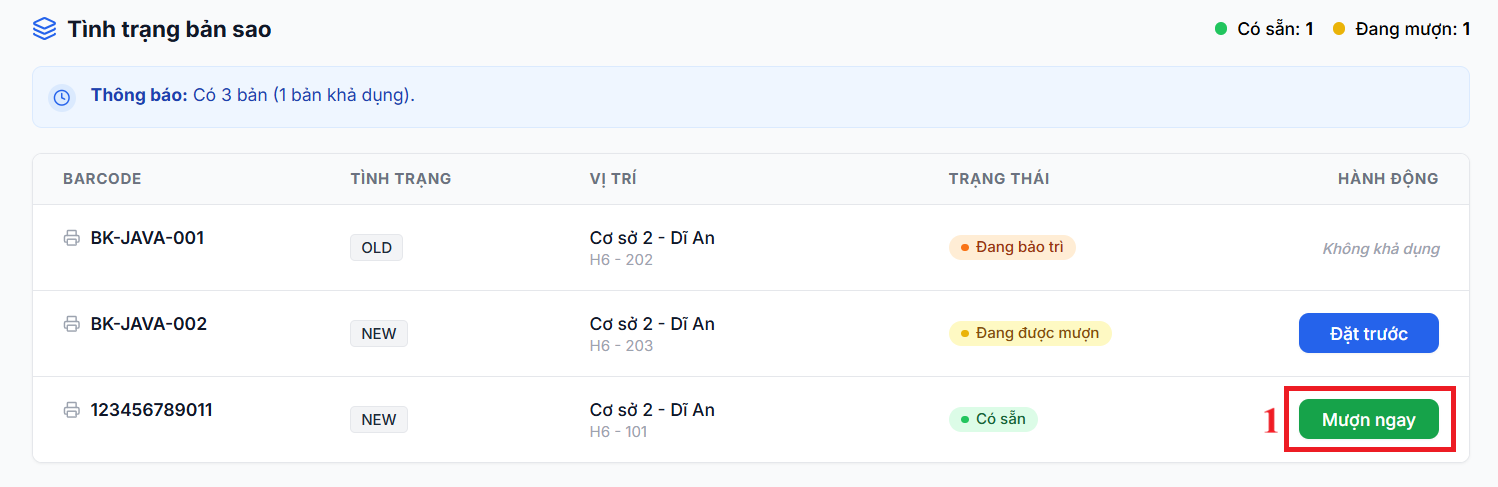
\includegraphics[width=\textwidth]{picture/muonsach/1nutmuonsach.png}
    \caption{Giao diện chọn bản sao và thực hiện mượn sách}
    \label{fig:borrow_button}
\end{figure}

\noindent\textbf{Mô tả giao diện:} 
Tại trang chi tiết ấn phẩm, độc giả có thể xem danh sách các bản sao vật lý hiện có tại từng cơ sở. Với những bản sao đang ở trạng thái "Có sẵn", hệ thống cung cấp nút thao tác "Mượn ngay". Nút này chỉ khả dụng khi hệ thống đánh giá người dùng đủ điều kiện mượn sách.

\begin{figure}[H]
    \centering
    \begin{minipage}{0.48\textwidth}
        \centering
        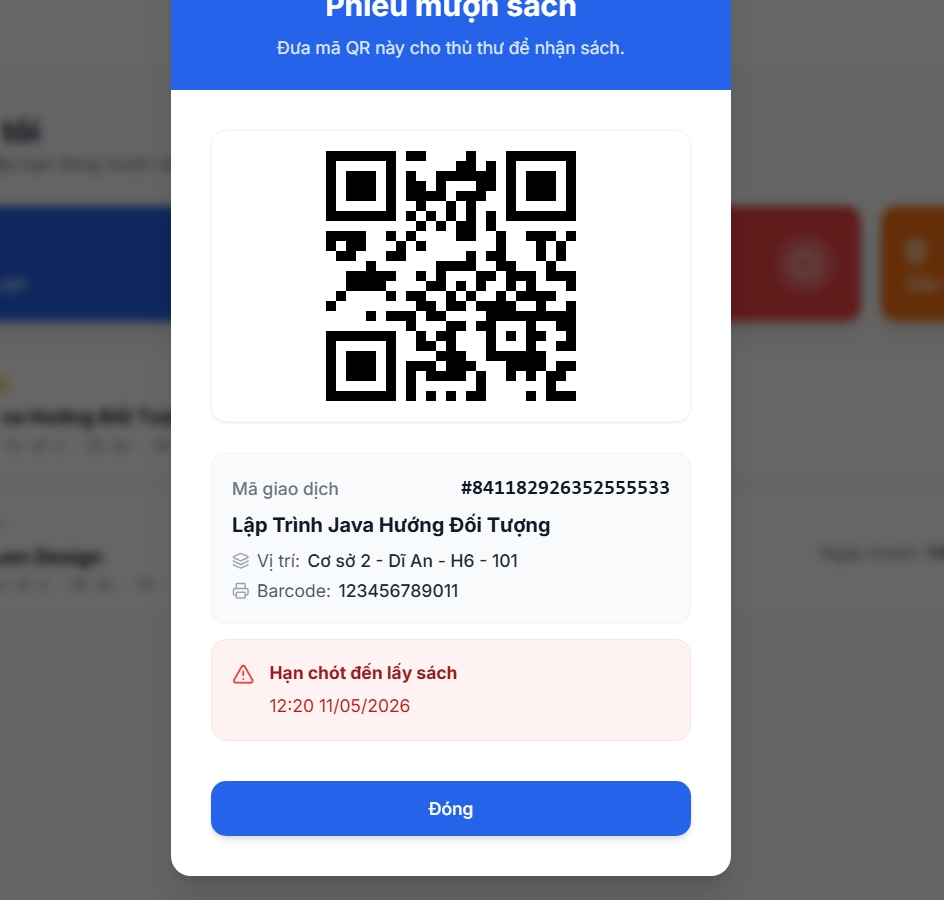
\includegraphics[width=\linewidth]{picture/muonsach/2phieumuonsaukhianmuonngay.jpeg}
        \caption{Phiếu mượn điện tử (Mã QR)}
        \label{fig:borrow_qr}
    \end{minipage}\hfill
    \begin{minipage}{0.48\textwidth}
        \centering
        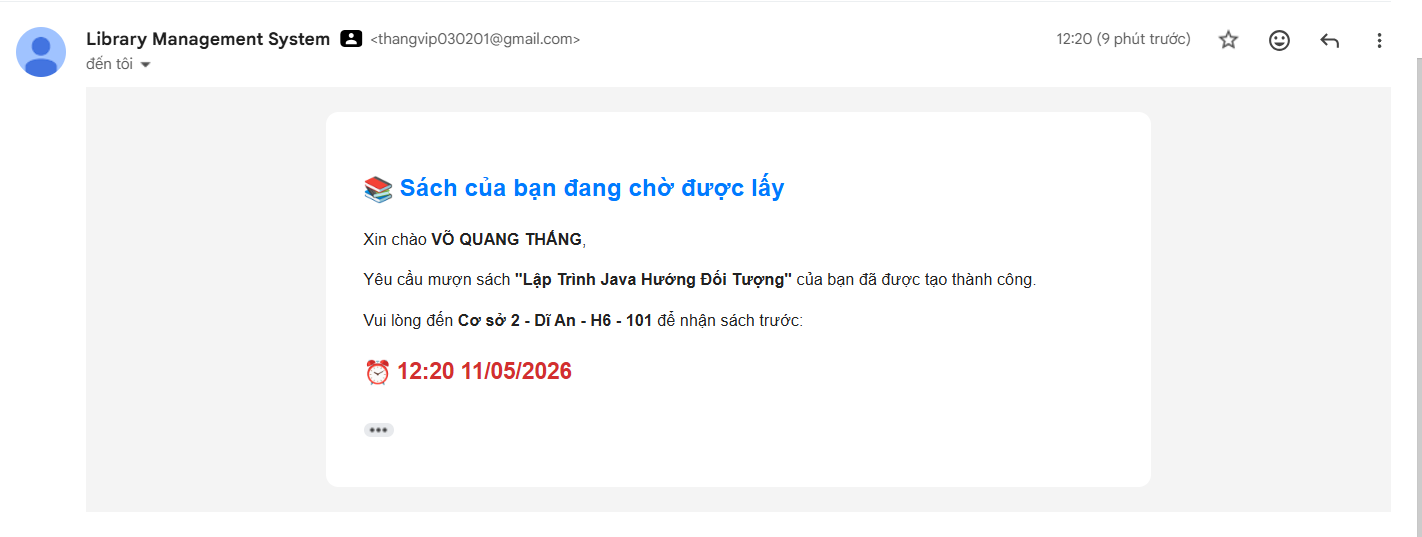
\includegraphics[width=\linewidth]{picture/muonsach/3emailnhacnho.png}
        \caption{Thư điện tử thông báo lịch hẹn}
        \label{fig:borrow_email}
    \end{minipage}
\end{figure}

\noindent\textbf{Mô tả nghiệp vụ:} 
Ngay khi độc giả nhấn "Mượn ngay", hệ thống sẽ khởi tạo một giao dịch đặt trước. Giao diện trả về một Phiếu mượn điện tử chứa mã QR, mã giao dịch, và hạn chót đến lấy sách (thường là 24 giờ kể từ lúc đặt). Đồng thời, một thư điện tử và thông báo đẩy sẽ được phát hành tự động để nhắc nhở người dùng lịch hẹn đến thư viện nhận sách.

\subsubsection{Luồng Thủ thư xử lý và giao sách tại quầy}

\begin{figure}[H]
    \centering
    \begin{minipage}{0.48\textwidth}
        \centering
        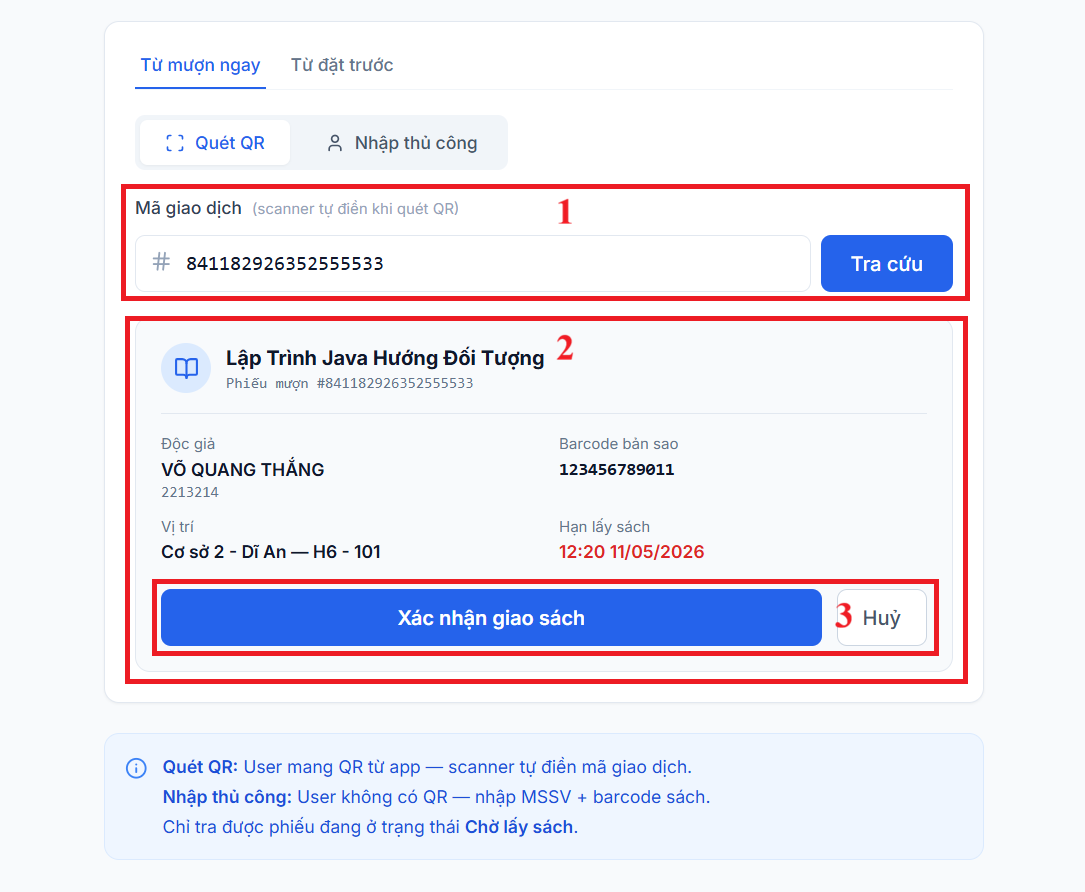
\includegraphics[width=\linewidth]{picture/muonsach/4thuthunhapvaomaphieudelookup.png}
        \caption{Tra cứu qua Mã giao dịch / Quét QR}
        \label{fig:borrow_lookup_qr}
    \end{minipage}\hfill
    \begin{minipage}{0.48\textwidth}
        \centering
        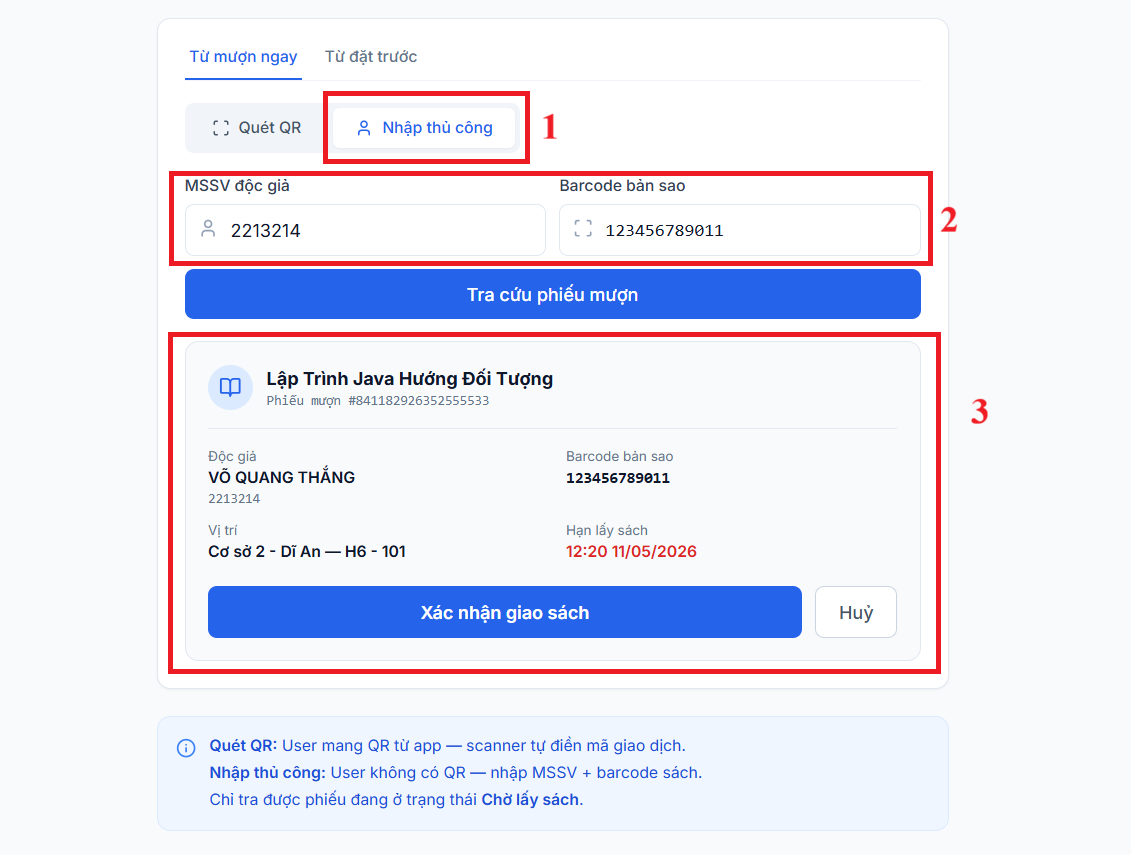
\includegraphics[width=\linewidth]{picture/muonsach/5hoaclalookupthongquanhapmssvvabarcode.png}
        \caption{Tra cứu thủ công qua Mã SV và Mã vạch sách}
        \label{fig:borrow_lookup_manual}
    \end{minipage}
\end{figure}

\noindent\textbf{Mô tả giao diện tra cứu:} 
Khi độc giả đến quầy, thủ thư sử dụng công cụ tra cứu để tìm lại giao dịch đặt trước. Hệ thống hỗ trợ hai phương thức linh hoạt: sử dụng máy quét mã vạch để quét trực tiếp mã QR trên ứng dụng của độc giả, hoặc nhập thủ công tổ hợp Mã số sinh viên và Mã vạch của cuốn sách. Nếu thông tin khớp, phiếu mượn sẽ hiển thị kèm nút "Xác nhận giao sách".

\begin{figure}[H]
    \centering
    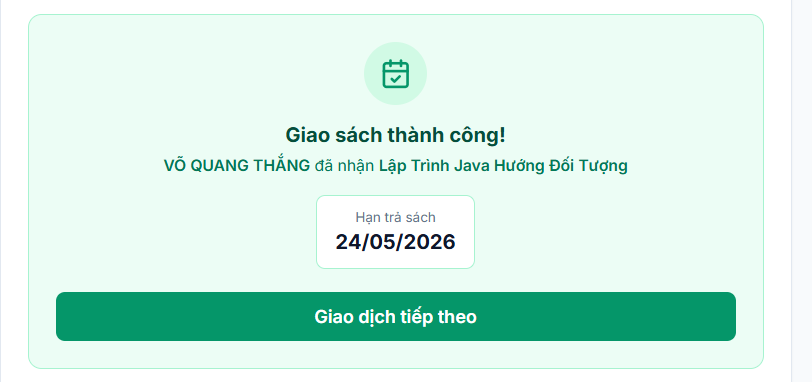
\includegraphics[width=0.7\textwidth]{picture/muonsach/6-xacnhangiaosachthanhcongothuthu.png}
    \caption{Màn hình thông báo giao sách thành công}
    \label{fig:borrow_success}
\end{figure}

\noindent\textbf{Mô tả nghiệp vụ giao sách:} 
Sau khi thủ thư kiểm tra vật lý và nhấn xác nhận, trạng thái giao dịch chính thức chuyển sang "Đang mượn". Màn hình hiển thị thông báo thành công kèm theo mốc thời gian hạn trả chính xác để thủ thư có thể nhắc nhở trực tiếp độc giả.

\vspace{0.5cm}
\subsubsection{Đặc tả API và Kỹ thuật}

Phân hệ mượn sách được vận hành bởi 4 giao tiếp (API) lõi, đảm bảo tính toàn vẹn dữ liệu thông qua các vòng kiểm duyệt chặt chẽ.

\noindent\textbf{1. Khởi tạo mượn sách trực tuyến (Web Flow)}
\begin{itemize}
    \item \textbf{Endpoint:} \texttt{POST /api/v1/transactions/borrow} (Quyền: Độc giả)
    \item \textbf{Kiểm duyệt điều kiện (Validation):} 
    Hệ thống thực hiện 4 rào chắn tuần tự: Bản sao phải có sẵn (\texttt{AVAILABLE}); Người dùng chưa đạt giới hạn mượn (tối đa 5 cuốn); Không có khoản phạt nào chưa thanh toán; và không được phép mượn trùng lặp một đầu sách đã đặt trước đó.
    \item \textbf{Chuyển đổi trạng thái:} Bản sao chuyển thành \texttt{RESERVED}. Giao dịch ở trạng thái \texttt{WAITING\_FOR\_PICKUP}.
    \item \textbf{Sự kiện (Event-driven):} Đẩy thông báo qua Kafka để kích hoạt dịch vụ gửi Email và App Notification.
\end{itemize}

\noindent\textbf{2. Tra cứu giao dịch tại quầy}
\begin{itemize}
    \item \textbf{Endpoint:} \texttt{GET /api/v1/transactions/lookup} (Quyền: Thủ thư)
    \item \textbf{Logic:} Tìm kiếm các giao dịch đang ở trạng thái \texttt{WAITING\_FOR\_PICKUP} thông qua mã giao dịch (ID) hoặc kết hợp Mã sinh viên và Mã vạch sách.
\end{itemize}

\noindent\textbf{3. Xác nhận giao sách (Hoàn tất Web Flow)}
\begin{itemize}
    \item \textbf{Endpoint:} \texttt{POST /api/v1/transactions/\{id\}/confirm-pickup} (Quyền: Thủ thư)
    \item \textbf{Logic:} Kiểm tra ID giao dịch hợp lệ. Cập nhật trạng thái giao dịch từ \texttt{WAITING\_FOR\_PICKUP} sang \texttt{BORROWING}. Cập nhật trạng thái bản sao từ \texttt{RESERVED} sang \texttt{BORROWED}. Ghi nhận thời gian mượn thực tế, mã số thủ thư giải quyết và thiết lập hạn trả (mặc định 14 ngày).
\end{itemize}

\noindent\textbf{4. Mượn trực tiếp tại quầy (Direct Flow)}
\begin{itemize}
    \item \textbf{Endpoint:} \texttt{POST /api/v1/transactions/borrow-direct} (Quyền: Thủ thư)
    \item \textbf{Logic:} Dành cho trường hợp độc giả lấy sách trực tiếp từ kệ ra quầy mà không đặt trước. Thủ thư nhập Mã sinh viên và Mã vạch. Hệ thống kiểm tra điều kiện tương tự luồng trực tuyến, nhưng bỏ qua giai đoạn chờ. Giao dịch được tạo và chuyển thẳng sang trạng thái \texttt{BORROWING}, bản sao chuyển sang \texttt{BORROWED}.
\end{itemize}




















% Preamble cần thiết: \usepackage{graphicx}, \usepackage{float}, \usepackage{tabularx}, \usepackage{booktabs}

\subsection{Nghiệp vụ Đặt trước sách}

Phân hệ Đặt trước sách (Reservation) là giải pháp giúp độc giả "xếp hàng" điện tử đối với những ấn phẩm đang tạm hết bản sao khả dụng tại thư viện. 

\subsubsection{Khởi tạo yêu cầu đặt trước}

\begin{figure}[H]
    \centering
    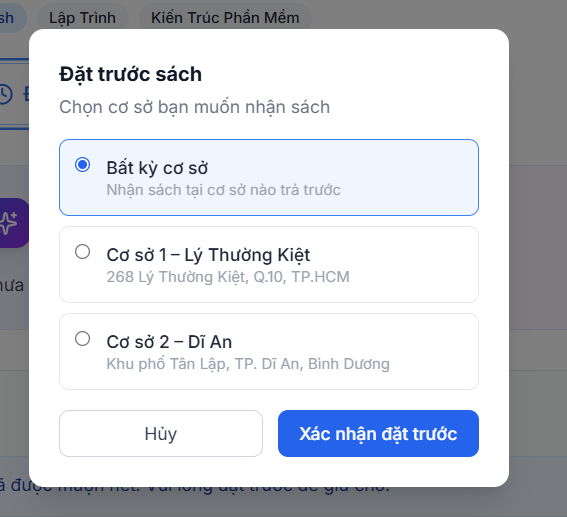
\includegraphics[width=0.65\textwidth]{picture/dattruocsach/1.png}
    \caption{Giao diện tùy chọn cơ sở nhận sách khi đặt trước}
    \label{fig:reserve_modal}
\end{figure}

\noindent\textbf{Mô tả giao diện:} Khi toàn bộ bản sao của một quyển sách đang được mượn, nút chức năng "Mượn ngay" sẽ được thay thế bằng "Đặt trước". Một hộp thoại sẽ xuất hiện yêu cầu độc giả chọn cơ sở mong muốn nhận sách. Người dùng có thể chọn một cơ sở cụ thể (như Lý Thường Kiệt hoặc Dĩ An) hoặc chọn "Bất kỳ cơ sở" để tối ưu hóa thời gian chờ đợi (nhận sách ở cơ sở nào có người trả sớm nhất).

\subsubsection{Quản lý danh sách đặt trước}

\begin{figure}[H]
    \centering
    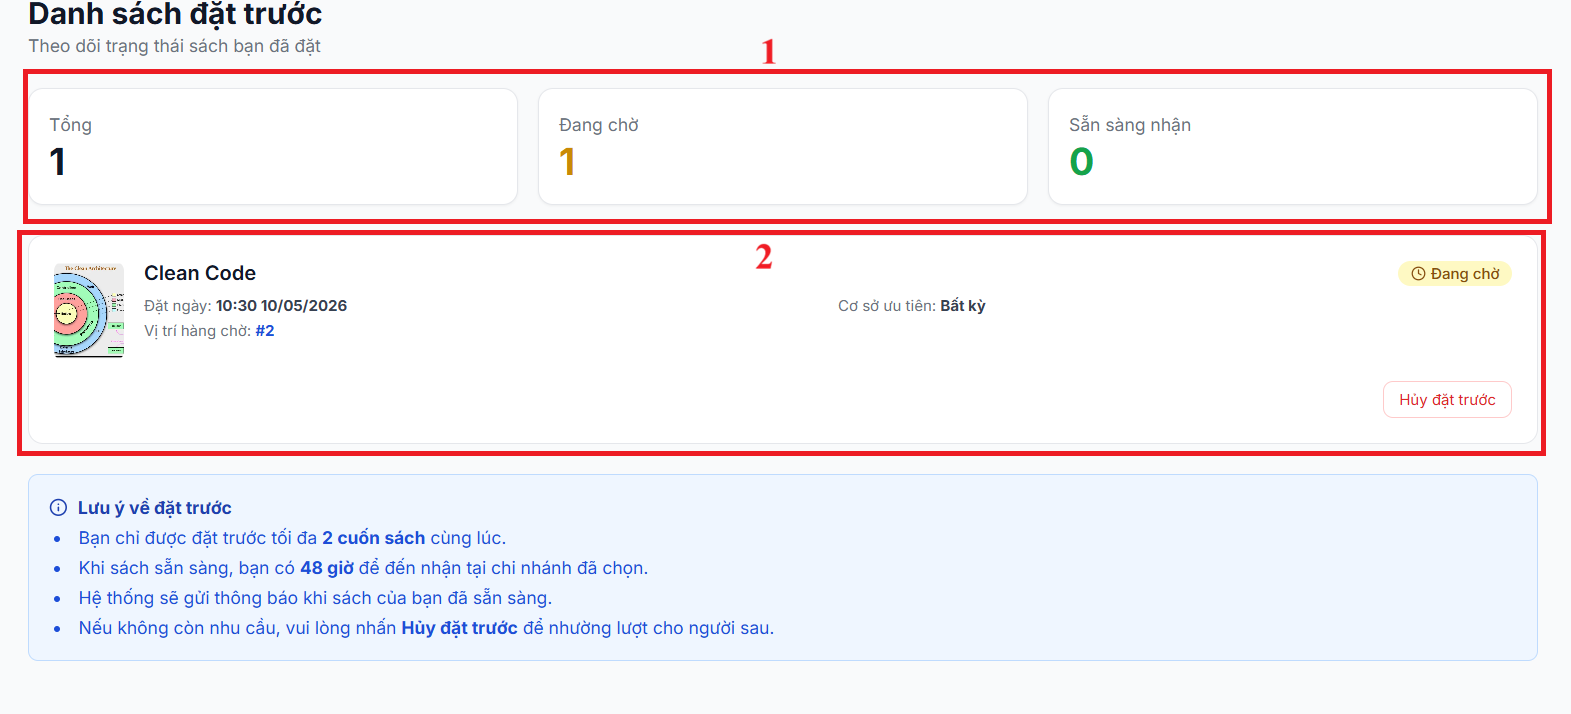
\includegraphics[width=\textwidth]{picture/dattruocsach/2.png}
    \caption{Trạng thái Đang chờ xếp hàng}
    \label{fig:reserve_list_pending}
\end{figure}

\noindent\textbf{Mô tả trạng thái Đang chờ:} 
Màn hình quản lý cung cấp một bộ đếm tổng quan về số lượng sách đang chờ và sẵn sàng. Ở trạng thái "Đang chờ", thẻ thông tin sẽ hiển thị rõ \textbf{vị trí hàng chờ} của độc giả (ví dụ: \#2 nghĩa là có 1 người khác đang xếp hàng trước). Hệ thống cũng liệt kê minh bạch các quy định: Mỗi người chỉ được đặt tối đa 2 cuốn cùng lúc và có thời hạn 48 giờ để đến nhận sách khi sách sẵn sàng. Tại đây, độc giả có thể chủ động hủy yêu cầu để nhường lượt cho người sau.

\begin{figure}[H]
    \centering
    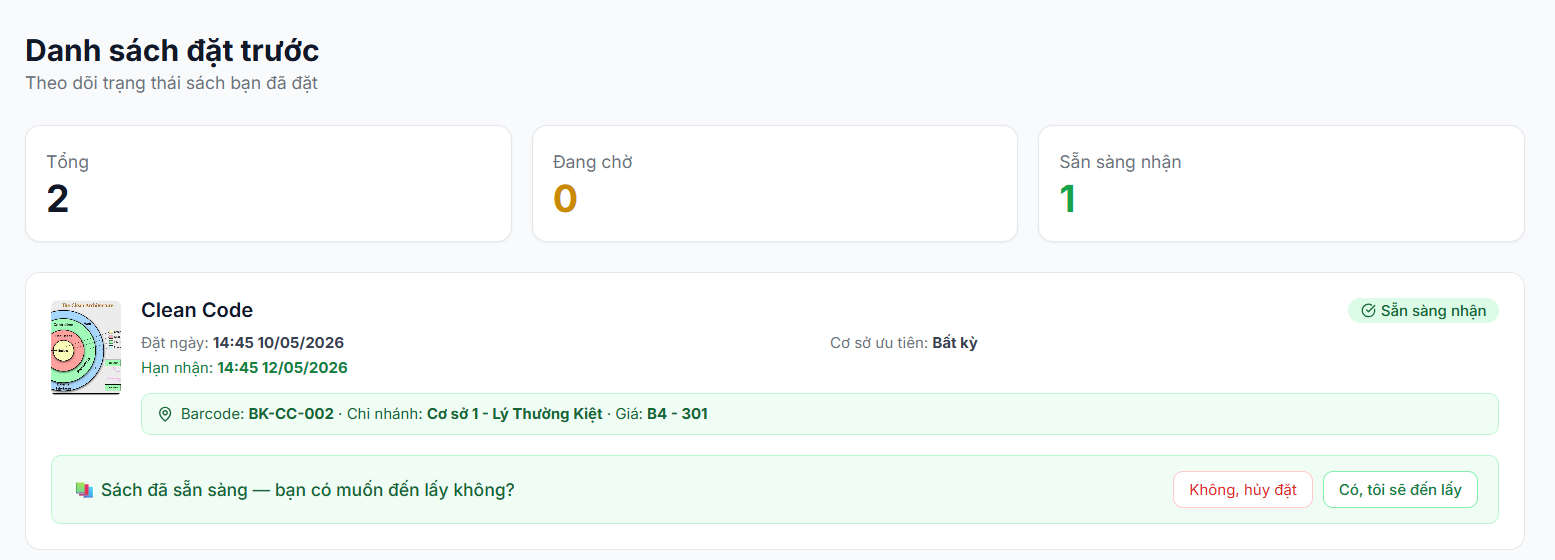
\includegraphics[width=\textwidth]{picture/dattruocsach/3.png}
    \caption{Trạng thái Sách sẵn sàng nhận}
    \label{fig:reserve_list_ready}
\end{figure}

\noindent\textbf{Mô tả trạng thái Sẵn sàng nhận:} 
Khi đến lượt, trạng thái thẻ chuyển sang "Sẵn sàng nhận" (màu xanh). Lúc này, hệ thống sẽ tiết lộ cụ thể mã vạch (barcode) của cuốn sách được phân bổ, chi nhánh và vị trí kệ sách chi tiết. Giao diện yêu cầu người dùng xác nhận lại việc đến lấy sách hoặc hủy bỏ.

\subsubsection{Hệ thống thông báo và Phiếu nhận}

\begin{figure}[H]
    \centering
    \begin{minipage}{0.48\textwidth}
        \centering
        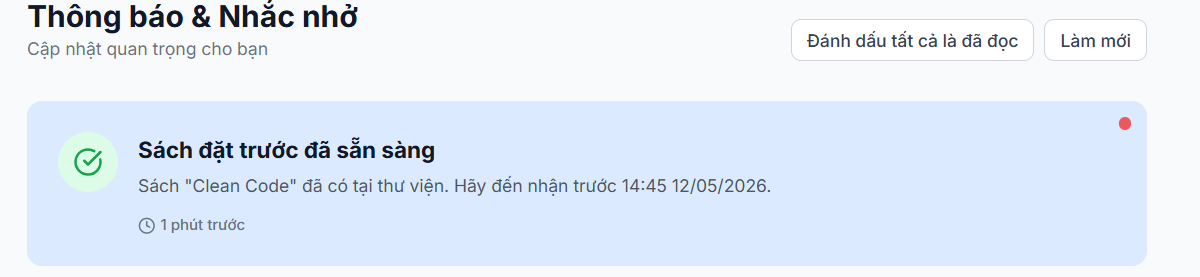
\includegraphics[width=\linewidth]{picture/dattruocsach/4.png}
        \caption{Thông báo cập nhật ngay trên trang web}
        \label{fig:reserve_noti_web}
    \end{minipage}\hfill
    \begin{minipage}{0.48\textwidth}
        \centering
        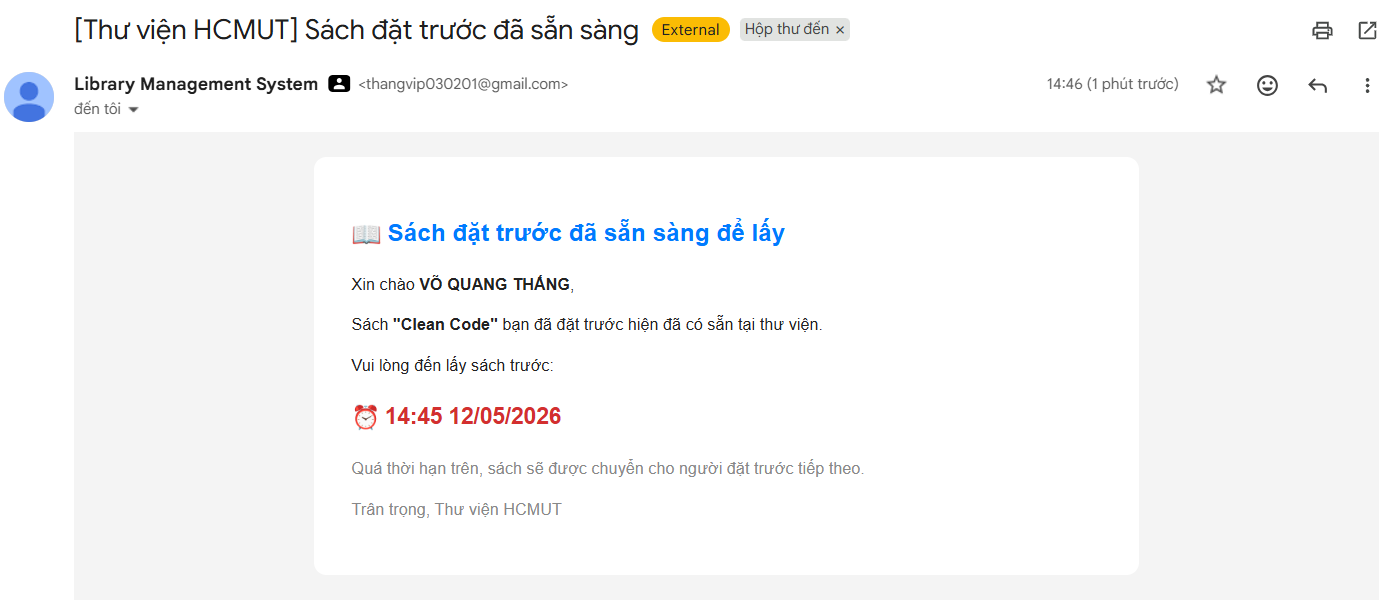
\includegraphics[width=\linewidth]{picture/dattruocsach/5.png}
        \caption{Thư điện tử thông báo sách đã về}
        \label{fig:reserve_noti_email}
    \end{minipage}
\end{figure}

\noindent\textbf{Luồng thông báo:} Ngay khi hệ thống cấp phát sách thành công, một thông báo đẩy thời gian thực và một thư điện tử sẽ được gửi song song đến độc giả, nhấn mạnh mốc thời gian hạn chót 48 giờ.

\begin{figure}[H]
    \centering
    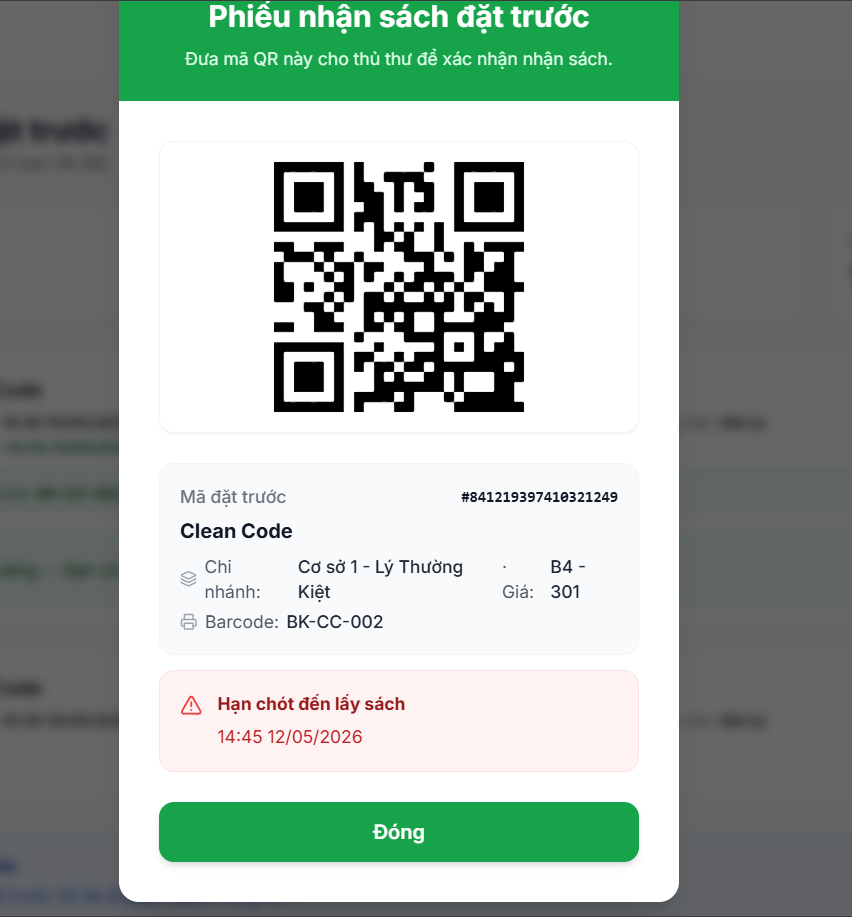
\includegraphics[width=0.55\textwidth]{picture/dattruocsach/6.png}
    \caption{Phiếu nhận sách điện tử (Mã QR)}
    \label{fig:reserve_qr}
\end{figure}

\noindent\textbf{Phiếu nhận sách:} Nếu độc giả xác nhận sẽ đến lấy ở Hình \ref{fig:reserve_list_ready}, một Phiếu nhận sách điện tử chứa mã QR sẽ được tạo ra, dùng để xuất trình cho thủ thư khi đến quầy.

\subsubsection{Xử lý giao sách tại quầy}

\begin{figure}[H]
    \centering
    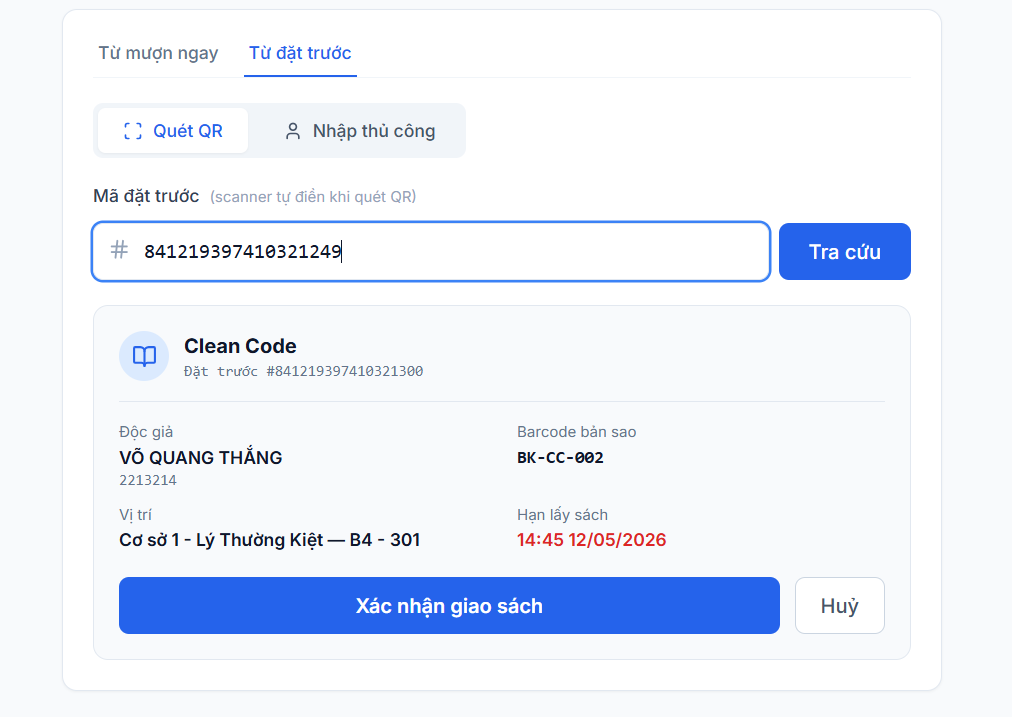
\includegraphics[width=0.7\textwidth]{picture/dattruocsach/7.png}
    \caption{Giao diện Thủ thư xác nhận giao sách đặt trước}
    \label{fig:reserve_librarian_confirm}
\end{figure}

\noindent\textbf{Luồng thủ thư:} Tại hệ thống dành cho nhân viên, thủ thư chuyển sang phân hệ "Từ đặt trước". Bằng cách quét mã QR của độc giả, hệ thống sẽ đối chiếu mã giao dịch và hiển thị thông tin bản sao đã được giữ sẵn. Thủ thư chỉ việc lấy đúng quyển sách trên kệ (dựa theo barcode hiển thị) và nhấn "Xác nhận giao sách". Giao dịch lúc này chính thức chuyển thành "Đang mượn".

\vspace{0.5cm}
\subsubsection{Đặc tả API và Kỹ thuật điều phối}

Tính năng đặt trước yêu cầu cơ chế xử lý đồng thời (Concurrency) rất khắt khe để tránh tình trạng tranh chấp dữ liệu khi nhiều sách được trả về cùng lúc.

\noindent\textbf{1. Khởi tạo yêu cầu đặt trước}
\begin{itemize}
    \item \textbf{Endpoint:} \texttt{POST /api/v1/reservations}
    \item \textbf{Kiểm duyệt (Validation):} Hệ thống áp dụng 5 tầng kiểm tra trước khi nhận đơn: Người dùng không nợ phí phạt; Chưa vượt hạn mức (tối đa 2 cuốn); Chưa đặt cuốn này trước đó; Thư viện phải sở hữu ít nhất 1 bản sao của sách này; và \textbf{quan trọng nhất}, toàn bộ các bản sao hiện tại đều không có sẵn (nếu có sẵn, hệ thống bắt lỗi và yêu cầu độc giả dùng tính năng Mượn ngay).
    \item \textbf{Xử lý hàng đợi:} Tính toán vị trí xếp hàng bằng công thức \texttt{MAX(queue\_position) + 1}. Trạng thái giao dịch khởi tạo là \texttt{PENDING}.
\end{itemize}

\noindent\textbf{2. Cơ chế phân bổ sách tự động (Assignment Service)}
\begin{itemize}
    \item Khi một bản sao được người dùng trước hoàn trả, hệ thống kích hoạt luồng kiểm tra hàng đợi đặt trước.
    \item \textbf{Tránh xung đột (Race Condition):} Truy vấn cơ sở dữ liệu sử dụng kỹ thuật khóa hàng \texttt{FOR UPDATE SKIP LOCKED}. Điều này đảm bảo nếu hai bản sao được trả lại cùng một tíc tắc, hai tiến trình máy chủ sẽ không phân bổ sách cho cùng một người đầu hàng đợi.
    \item \textbf{Cập nhật trạng thái:} Người đầu tiên trong hàng đợi (ưu tiên theo chi nhánh) sẽ được gán \texttt{assignedItemId}. Trạng thái chuyển sang \texttt{READY\_FOR\_PICKUP}. Hệ thống thiết lập \texttt{holdExpirationTime} là thời điểm hiện tại cộng thêm 48 giờ, đồng thời bắn sự kiện qua Kafka để gửi thư thông báo.
\end{itemize}

\noindent\textbf{3. Hủy hoặc quá hạn đặt trước}
\begin{itemize}
    \item \textbf{Endpoint:} \texttt{DELETE /api/v1/reservations/\{id\}}
    \item \textbf{Logic:} Nếu độc giả chủ động hủy, hoặc hệ thống quét thấy đã quá 48 giờ mà chưa nhận, giao dịch hiện tại sẽ chuyển sang \texttt{CANCELLED} hoặc \texttt{EXPIRED}. Ngay lập tức, bản sao vừa được giải phóng sẽ lại kích hoạt luồng Phân bổ tự động (bước 2) để nhường lượt cho người đang đứng thứ 2 trong hàng đợi.
\end{itemize}





% Preamble cần thiết: \usepackage{graphicx}, \usepackage{float}, \usepackage{tabularx}, \usepackage{booktabs}

\subsection{Đánh giá và Nhận xét ấn phẩm}

\subsubsection{Giao diện Hệ thống đánh giá}

\begin{figure}[H]
    \centering
    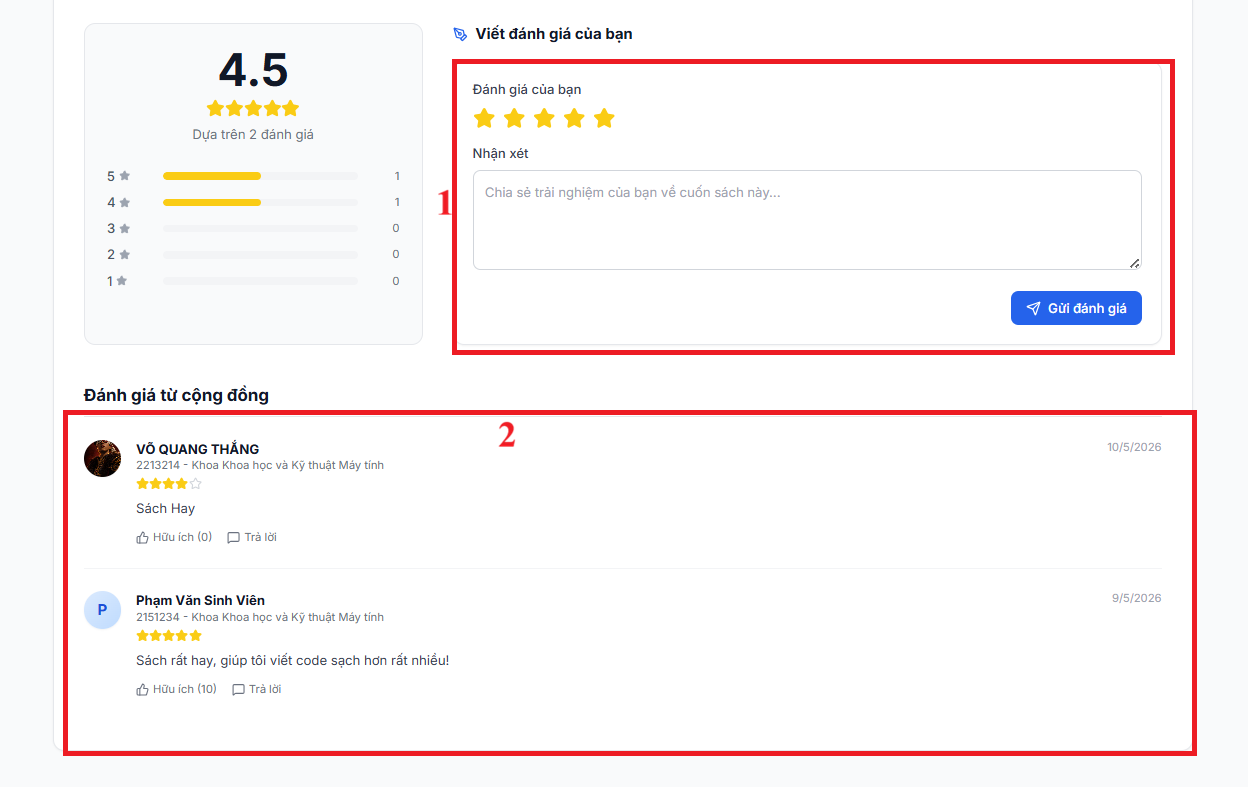
\includegraphics[width=\textwidth]{picture/danhgiaanpham/1.png}
    \caption{Giao diện Đánh giá và Nhận xét từ cộng đồng độc giả}
    \label{fig:publication_rating}
\end{figure}

\noindent\textbf{Chú thích các vùng chức năng:}
\begin{itemize}
    \item \textbf{Khối Thống kê tổng quan (Bên trái):} Trình bày điểm đánh giá trung bình của ấn phẩm và thanh tiến trình phân bổ số lượng chi tiết cho từng mức sao (từ 1 đến 5).
    \item \textbf{Vùng 1 (Biểu mẫu tương tác):} Khu vực cho phép độc giả chủ động để lại nhận xét. Hệ thống yêu cầu người dùng chọn mức độ hài lòng thông qua hệ thống 5 sao và bắt buộc phải nhập nội dung chia sẻ trải nghiệm đọc.
    \item \textbf{Vùng 2 (Danh sách cộng đồng):} Hiển thị dòng thời gian các đánh giá từ những độc giả khác. Mỗi nhận xét đều được minh bạch hóa thông qua việc đính kèm thông tin định danh của người viết, bao gồm ảnh đại diện, họ tên, mã số sinh viên, khoa trực thuộc và thời gian đăng tải.
\end{itemize}

\vspace{0.5cm}
\subsubsection{Đặc tả API và Ràng buộc nghiệp vụ}

Hệ thống đánh giá được thiết kế như một mô-đun độc lập nhằm tối ưu hóa hiệu suất truy vấn. Đường dẫn gốc phục vụ giao tiếp nghiệp vụ này là \texttt{/api/v1/publications/\{publicationId\}/ratings}.

\noindent\textbf{1. Ràng buộc cốt lõi khi tạo đánh giá}
\begin{itemize}
    \item \textbf{Xác thực quyền hạn:} Chỉ những người dùng đã xác thực (đăng nhập) mới được phép sử dụng điểm cuối của phân hệ này để tạo mới đánh giá.
    \item \textbf{Điều kiện thực tiễn:} Để đảm bảo tính khách quan của nền tảng, thuật toán kiểm duyệt sẽ đối chiếu lịch sử giao dịch. Độc giả \textbf{bắt buộc phải từng mượn} ấn phẩm này thì mới có quyền để lại nhận xét. Nếu vi phạm, hệ thống sẽ từ chối và trả về mã lỗi \texttt{USER\_NOT\_BORROWED\_PUBLICATION}.
    \item \textbf{Tính duy nhất:} Mỗi độc giả chỉ được phép đánh giá một lần duy nhất cho mỗi đầu sách. Việc cố tình gửi yêu cầu trùng lặp sẽ bị chặn lại bởi ràng buộc dữ liệu kèm mã lỗi \texttt{RATING\_ALREADY\_EXISTS}.
\end{itemize}

\noindent\textbf{2. Tối ưu hóa tải trang giao diện}
\begin{itemize}
    \item Khi độc giả truy cập vào tab Đánh giá, giao diện mạng (Frontend) sẽ tiến hành gọi đồng thời (song song) hai giao tiếp: một truy vấn để lấy dữ liệu thống kê tổng hợp và một truy vấn khác để lấy danh sách bình luận phân trang. Điều này giúp giảm thiểu độ trễ tải trang.
    \item Ngay sau khi người dùng gửi đánh giá mới thành công, toàn bộ giao diện (bao gồm cả khối thống kê và danh sách bình luận) sẽ tự động làm mới để phản ánh dữ liệu tức thời.
\end{itemize}

\subsection{Lịch sử tìm kiếm}

\subsubsection{Giao diện hiển thị}

\begin{figure}[H]
    \centering
    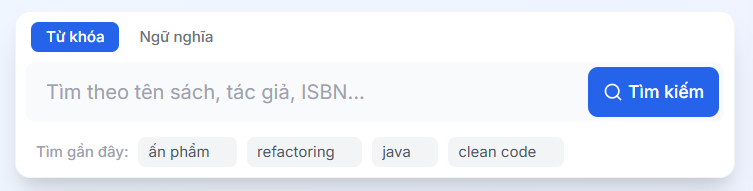
\includegraphics[width=\textwidth]{picture/lichsutimkiem/1.png}
    \caption{Giao diện gợi ý từ khóa tìm kiếm gần đây tại Trang chủ}
    \label{fig:search_history_chips}
\end{figure}

\noindent\textbf{Mô tả giao diện tại Trang chủ:} 
Ngay bên dưới thanh tìm kiếm chính, hệ thống cung cấp một danh sách các từ khóa mà độc giả đã tìm kiếm gần đây nhất, được trình bày dưới dạng các thẻ (chips) trực quan. Khi người dùng nhấn vào một thẻ, hệ thống sẽ tự động điền từ khóa đó vào ô tìm kiếm và thực hiện lệnh tra cứu ngay lập tức. Ngoài ra, khi di chuột lên từng thẻ, một biểu tượng dấu tắt (×) sẽ xuất hiện cho phép người dùng xóa nhanh từ khóa đó khỏi lịch sử.

\begin{figure}[H]
    \centering
    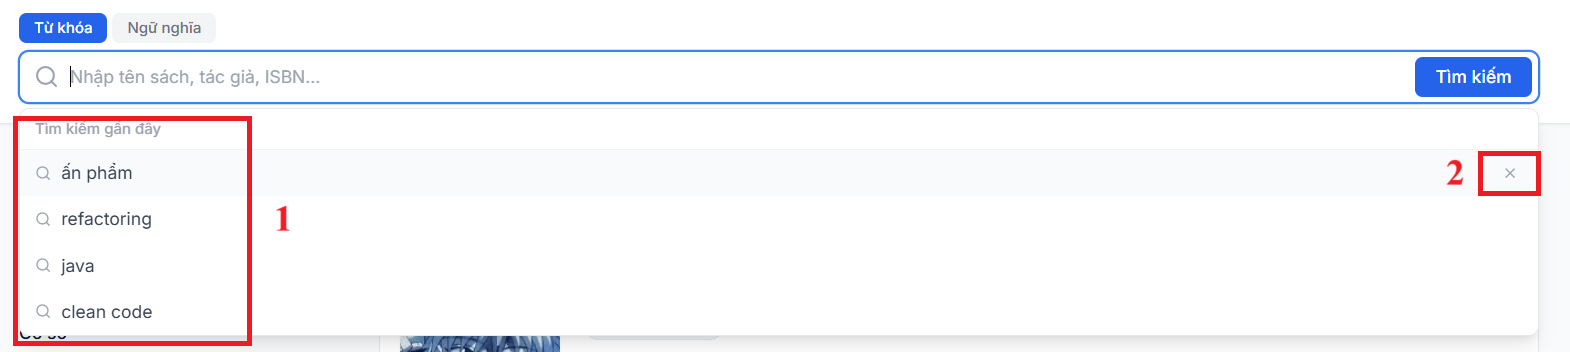
\includegraphics[width=\textwidth]{picture/lichsutimkiem/2.png}
    \caption{Danh sách thả xuống quản lý lịch sử tại Trang tìm kiếm}
    \label{fig:search_history_dropdown}
\end{figure}

\noindent\textbf{Chú thích các vùng chức năng tại Trang tìm kiếm:}
\begin{itemize}
    \item \textbf{Vùng 1 (Danh sách từ khóa):} Khi người dùng nhấp chuột (focus) vào thanh tìm kiếm, một danh sách thả xuống sẽ xuất hiện, hiển thị tối đa 10 từ khóa tra cứu gần nhất. Quá trình này diễn ra mượt mà và tự động lọc các kết quả tương đồng (gợi ý) ngay khi người dùng bắt đầu gõ từng ký tự.
    \item \textbf{Vùng 2 (Công cụ gỡ bỏ):} Nút thao tác nhanh giúp độc giả chủ động xóa từng lịch sử riêng lẻ. Thao tác này sẽ làm mới danh sách hiển thị ngay lập tức.
\end{itemize}

\vspace{0.5cm}
\subsubsection{Đặc tả giao tiếp hệ thống và Xử lý nghiệp vụ}

Phân hệ này hoạt động dựa trên 3 luồng giao tiếp dữ liệu chính. Toàn bộ các điểm cuối đều yêu cầu người dùng phải đăng nhập hợp lệ để đảm bảo tính cá nhân hóa.

\noindent\textbf{1. Ghi nhận và Lưu trữ từ khóa}
\begin{itemize}
    \item \textbf{Điểm cuối:} \texttt{POST /api/v1/search-history} 
    \item \textbf{Mô tả luồng xử lý (Upsert):} Khi người dùng nhấn "Tìm kiếm", hệ thống sẽ âm thầm gửi từ khóa về máy chủ mà không làm gián đoạn trải nghiệm (không chặn giao diện). Thuật toán lưu trữ được thiết kế tối ưu như sau:
    \begin{itemize}
        \item Hệ thống bỏ qua các từ khóa rỗng.
        \item Nếu từ khóa đã từng được tìm kiếm trước đó, hệ thống chỉ cập nhật lại mốc thời gian và đẩy từ khóa này lên vị trí đầu tiên.
        \item Nếu là từ khóa mới, hệ thống sẽ kiểm tra giới hạn lưu trữ. Mỗi tài khoản chỉ được lưu tối đa 10 từ khóa. Nếu vượt quá, máy chủ sẽ tự động tìm và xóa bản ghi cũ nhất trước khi thêm bản ghi mới.
    \end{itemize}
\end{itemize}

\noindent\textbf{2. Truy xuất danh sách lịch sử}
\begin{itemize}
    \item \textbf{Điểm cuối:} \texttt{GET /api/v1/search-history}    \item \textbf{Mô tả luồng xử lý:} Giao tiếp này phục vụ cả việc lấy 10 từ khóa gần nhất (khi ô tìm kiếm trống) và tính năng tự động gợi ý (khi người dùng đang gõ). Dữ liệu trả về luôn được sắp xếp ưu tiên theo mốc thời gian cập nhật mới nhất.
\end{itemize}

\noindent\textbf{3. Gỡ bỏ từ khóa}
\begin{itemize}
    \item \textbf{Điểm cuối:} \texttt{DELETE /api/v1/search-history/\{id\}}     \item \textbf{Mô tả luồng xử lý:} Người dùng có thể xóa một lịch sử cụ thể thông qua mã định danh. Máy chủ sẽ xác minh quyền sở hữu (đảm bảo người dùng không xóa lịch sử của người khác) trước khi thực thi lệnh.
\end{itemize}

% Preamble cần thiết: \usepackage{graphicx}, \usepackage{float}, \usepackage{tabularx}, \usepackage{booktabs}

\subsection{Hệ thống Thông báo và Nhắc nhở (Real-time Notifications)}

\subsubsection{Giao diện Trung tâm thông báo}

\begin{figure}[H]
    \centering
    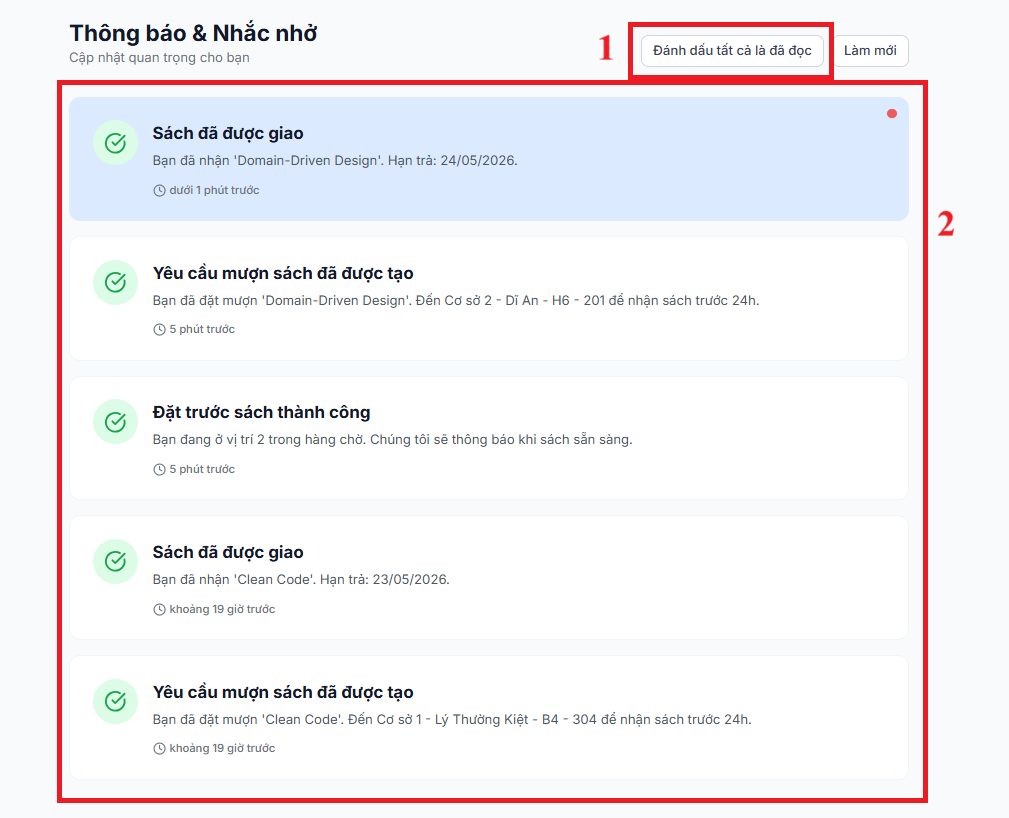
\includegraphics[width=\textwidth]{picture/notification/2giaodien.png}
    \caption{Giao diện quản lý Thông báo và Nhắc nhở dành cho Độc giả}
    \label{fig:notification_ui}
\end{figure}

\noindent\textbf{Chú thích các vùng chức năng:}
\begin{itemize}
    \item \textbf{Vùng 1 (Thanh công cụ):} Cung cấp các thao tác quản lý nhanh, bao gồm nút "Đánh dấu tất cả là đã đọc" giúp làm sạch giao diện ngay lập tức và nút "Làm mới" để tải lại dữ liệu thủ công nếu cần.
    \item \textbf{Vùng 2 (Danh sách thông báo):} Hiển thị dòng thời gian các sự kiện liên quan trực tiếp đến người dùng. Mỗi thẻ thông báo được thiết kế trực quan với biểu tượng tương ứng với loại sự kiện (ví dụ: Tạo yêu cầu mượn, Giao sách thành công, Đặt trước sẵn sàng). Những thông báo chưa đọc sẽ được làm nổi bật bằng lớp nền xanh nhạt và một chấm đỏ ở góc phải, giúp độc giả dễ dàng nhận diện.
\end{itemize}

\vspace{0.5cm}
\subsubsection{Đặc tả Kiến trúc và Luồng xử lý thời gian thực}

Để mang lại trải nghiệm liền mạch, hệ thống thông báo được thiết kế dựa trên kiến trúc hướng sự kiện (Event-driven Architecture) kết hợp với công nghệ truyền tải hai chiều (WebSocket).

\noindent\textbf{1. Hạ tầng kỹ thuật cốt lõi}
\begin{itemize}
    \item \textbf{Cơ chế hàng đợi (Kafka):} Bất cứ khi nào có một nghiệp vụ phát sinh từ các phân hệ khác (như mượn trả sách, bộ lập lịch quét quá hạn), máy chủ sẽ đóng gói một thông điệp và đẩy vào chủ đề (topic) \texttt{notification.send} của Kafka.
    \item \textbf{Truyền tải thời gian thực (WebSocket STOMP):} Hệ thống sử dụng giao thức STOMP trên nền SockJS để duy trì kết nối liên tục với trình duyệt của người dùng. Tính bảo mật được đảm bảo tuyệt đối bằng cách đính kèm chuỗi định danh (JWT) ngay trong phần tiêu đề (headers) khi khởi tạo kết nối.
    \item \textbf{Lưu trữ tối ưu:} Cơ sở dữ liệu được tách làm hai bảng riêng biệt: \texttt{notifications} dùng để lưu trữ nội dung thông báo chung (tiêu đề, nội dung, đường dẫn), và \texttt{user\_notifications} để ánh xạ và theo dõi trạng thái "Đã đọc / Chưa đọc" của từng cá nhân.
\end{itemize}

\noindent\textbf{2. Vòng đời của một Thông báo}
\begin{enumerate}
    \item \textbf{Phát sinh:} Phân hệ xử lý trung tâm (Consumer) nhận thông điệp từ Kafka, lưu nội dung vào cơ sở dữ liệu và ngay lập tức đẩy (push) dữ liệu qua kênh WebSocket cá nhân hóa (\texttt{/queue/notifications}) của người dùng.
    \item \textbf{Tiếp nhận hiển thị:} Trình duyệt của người dùng nhận dữ liệu, tự động đẩy thông báo mới lên đầu danh sách, tăng bộ đếm số lượng chưa đọc, đồng thời hiển thị một thẻ thông báo nổi (Toast) với màu sắc được phân loại theo mức độ quan trọng.
    \item \textbf{Khởi động hệ thống:} Ngay khi người dùng đăng nhập thành công, ứng dụng mạng (Frontend) sẽ thiết lập kết nối WebSocket có hỗ trợ tự động kết nối lại (auto-reconnect) sau 5 giây nếu mạng gián đoạn. Song song đó, hệ thống gọi API để lấy 20 thông báo gần nhất và cập nhật bộ đếm.
\end{enumerate}

\subsubsection{Đặc tả Giao tiếp dữ liệu (API)}

\begin{figure}[H]
    \centering
    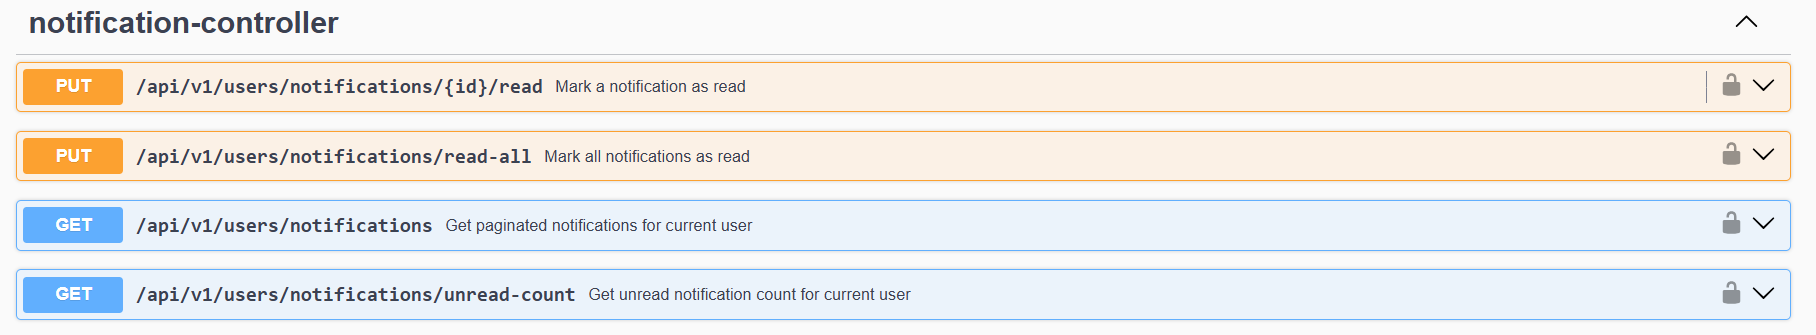
\includegraphics[width=\textwidth]{picture/notification/1api.png}
    \caption{Tập hợp các điểm cuối (Endpoints) của phân hệ Thông báo}
    \label{fig:notification_api}
\end{figure}

Hệ thống quản lý trạng thái thông báo thông qua 4 điểm cuối chính thuộc \texttt{/api/v1/users/notifications}:

\begin{table}[H]
    \centering
    \caption{Danh sách API Quản lý thông báo}
    \renewcommand{\arraystretch}{1.3}
    \begin{tabularx}{\textwidth}{|l|l|X|}
        \hline
        \textbf{Phương thức} & \textbf{Đường dẫn (Path)} & \textbf{Mô tả nghiệp vụ} \\ \hline
        GET & \texttt{/} & Truy xuất danh sách thông báo của người dùng kèm phân trang. \\ \hline
        GET & \texttt{/unread-count} & Trả về con số thống kê các thông báo chưa được đọc. \\ \hline
        PUT & \texttt{/\{id\}/read} & Đánh dấu một thông báo cụ thể là "Đã đọc". \\ \hline
        PUT & \texttt{/read-all} & Đánh dấu toàn bộ thông báo của người dùng là "Đã đọc". \\ \hline
    \end{tabularx}
\end{table}

\noindent\textbf{Tối ưu trải nghiệm:} 
Khi người dùng nhấp vào một thông báo hoặc chọn "Đánh dấu tất cả là đã đọc", giao diện (Frontend) sẽ ngay lập tức chuyển trạng thái hiển thị (tắt chấm đỏ, giảm bộ đếm) mà không cần chờ phản hồi từ máy chủ. Yêu cầu cập nhật cơ sở dữ liệu sẽ được gửi ngầm song song ở chế độ nền thông qua các lệnh \texttt{PUT}, giúp thao tác của người dùng luôn đạt độ trễ tiệm cận bằng không.


% Preamble cần thiết: \usepackage{graphicx}, \usepackage{float}, \usepackage{tabularx}, \usepackage{booktabs}

\subsection{Nghiệp vụ Trả sách và Xử lý sự cố}

\subsubsection{Giao diện Tra cứu và Trả sách}

\begin{figure}[H]
    \centering
    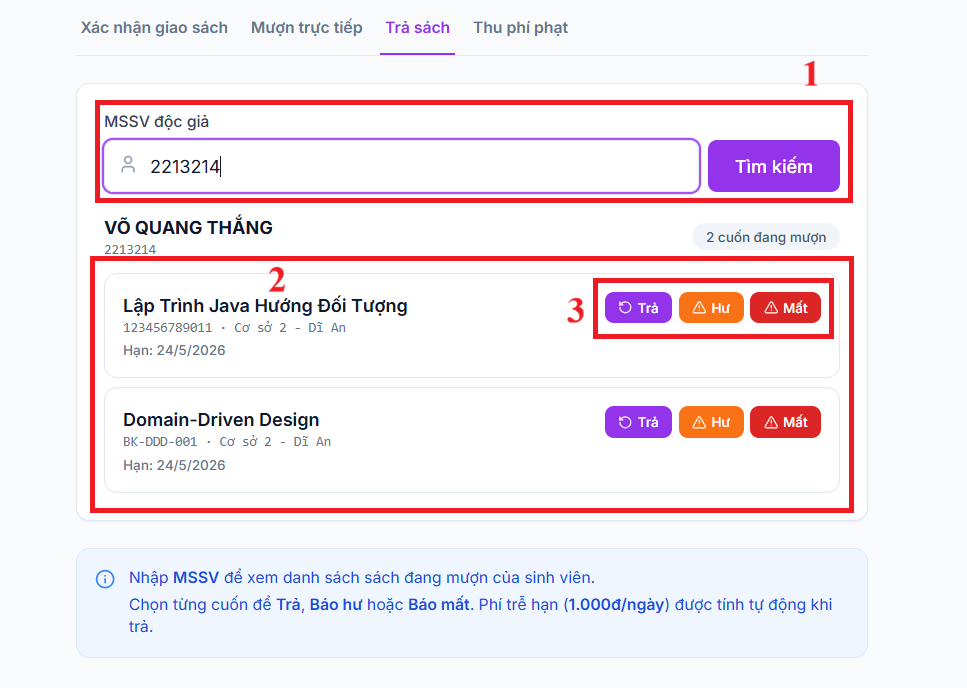
\includegraphics[width=\textwidth]{picture/trasach/1thuthunhapmssvdetracuusachdangmuon.png}
    \caption{Giao diện nhập thông tin để tra cứu sách đang mượn}
    \label{fig:return_lookup}
\end{figure}

\noindent\textbf{Chú thích giao diện:} Tại phân hệ dành cho thủ thư, hệ thống cho phép tra cứu nhanh các giao dịch đang mượn thông qua Mã số sinh viên (MSSV). Danh sách trả về hiển thị rõ các ấn phẩm mà độc giả đang giữ, đi kèm với các nút thao tác tương ứng: "Trả" (hoàn trả bình thường), "Hư" (báo cáo hư hỏng) và "Mất" (báo cáo thất lạc).

\begin{figure}[H]
    \centering
    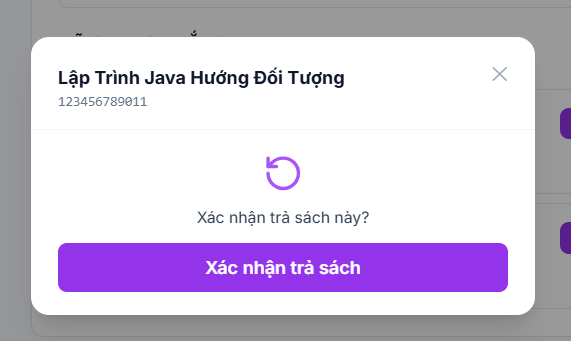
\includegraphics[width=0.6\textwidth]{picture/trasach/2popupxacnhantracuathuthu.png}
    \caption{Hộp thoại xác nhận hoàn trả tài liệu}
    \label{fig:return_confirm}
\end{figure}

\noindent\textbf{Nghiệp vụ hoàn trả cơ bản:} Khi thủ thư chọn "Trả", một hộp thoại xác nhận sẽ xuất hiện để đối chiếu thông tin sách và mã vạch lần cuối. Nếu giao dịch hoàn tất thành công, trạng thái của bản sao sẽ ngay lập tức được chuyển về "Có sẵn" (AVAILABLE. Trong trường hợp độc giả trả sách quá hạn, hệ thống sẽ tự động tính toán phí phạt dựa trên công thức số ngày trễ nhân với 1.000 VNĐ/ngày.

\subsubsection{Xử lý sự cố Hư hỏng và Mất sách}

\begin{figure}[H]
    \centering
    \begin{minipage}{0.48\textwidth}
        \centering
        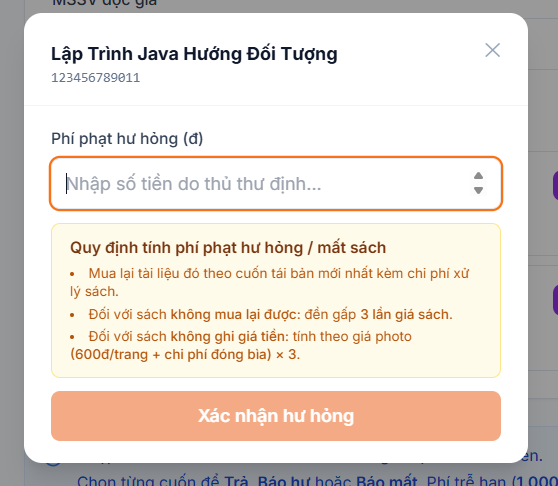
\includegraphics[width=\linewidth]{picture/trasach/3popupbaohuvasotiensinhviencanden.png}
        \caption{Hộp thoại xử lý báo cáo hư hỏng sách}
        \label{fig:return_damaged}
    \end{minipage}\hfill
    \begin{minipage}{0.48\textwidth}
        \centering
        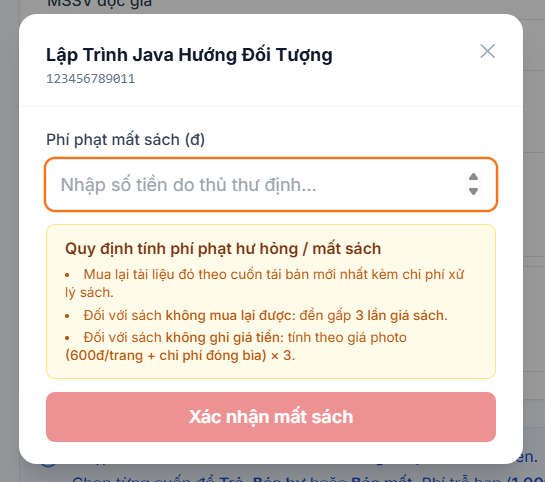
\includegraphics[width=\linewidth]{picture/trasach/4popupmatsach.png}
        \caption{Hộp thoại xử lý báo cáo mất sách}
        \label{fig:return_lost}
    \end{minipage}
\end{figure}

\noindent\textbf{Quy trình xử lý ngoại lệ:} 
Khi xảy ra sự cố vật lý với bản sao, thủ thư sẽ sử dụng tính năng "Hư" hoặc "Mất". Hệ thống cung cấp một biểu mẫu để thủ thư nhập số tiền phạt cụ thể dựa trên quy định bồi thường của thư viện (ví dụ: đền gấp 3 lần giá sách đối với sách không mua lại được). Trạng thái bản sao sẽ lập tức bị khóa, chuyển thành Đang bảo trì (IN\_MAINTENANCE) hoặc Thất lạc (LOST), đảm bảo không có giao dịch đặt trước nào được phép khởi tạo trên bản sao này.

\subsubsection{Hệ thống thông báo và Xác nhận}

\begin{figure}[H]
    \centering
    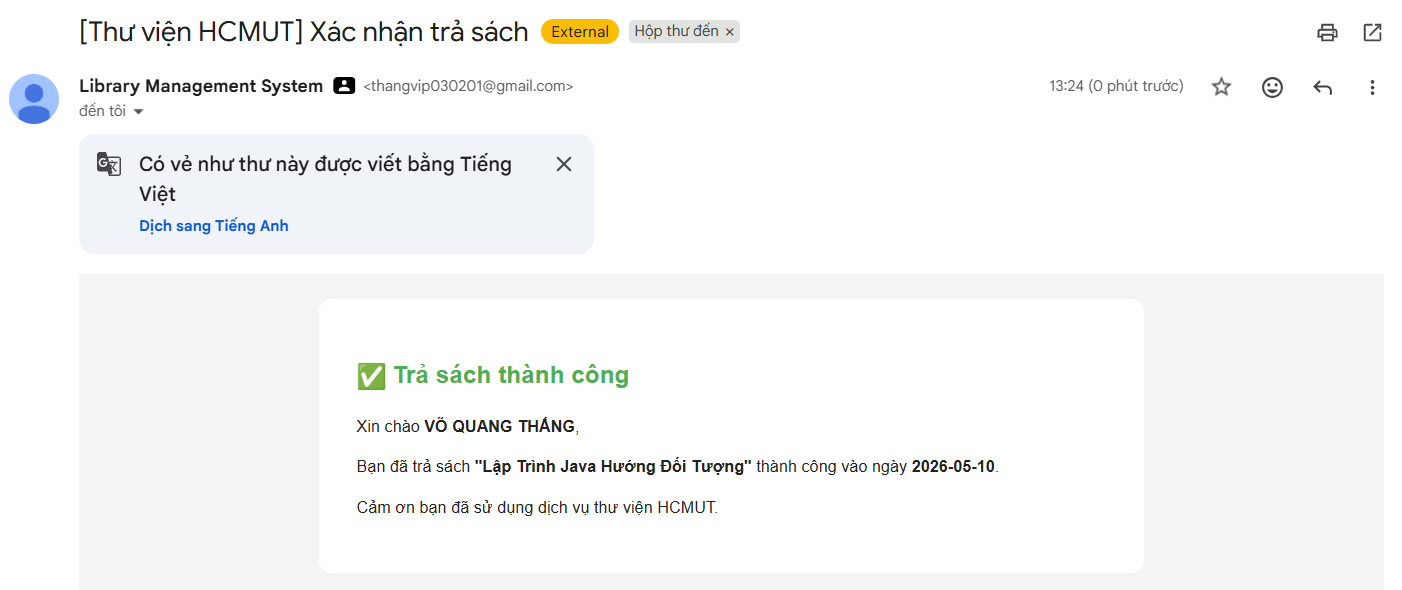
\includegraphics[width=0.9\textwidth]{picture/trasach/5guiemailxacnhanchodocgia.png}
    \caption{Thư điện tử xác nhận giao dịch trả sách thành công}
    \label{fig:return_email}
\end{figure}

\noindent\textbf{Mô tả luồng thông báo:} Ngay sau khi thủ thư xác nhận trả sách trên hệ thống, một sự kiện (event) sẽ được kích hoạt thông qua Kafka. Độc giả sẽ lập tức nhận được một thư điện tử biên nhận, ghi rõ thời gian hoàn tất giao dịch để lưu trữ và đối soát.

\vspace{0.5cm}
\subsubsection{Đặc tả API và Kỹ thuật điều phối}

Phân hệ trả sách yêu cầu xử lý logic phức tạp để đảm bảo tính nhất quán dữ liệu, đặc biệt là cơ chế khóa chống tranh chấp (Pessimistic Lock).

\noindent\textbf{1. Truy xuất thông tin giao dịch}
\begin{itemize}
    \item \textbf{Điểm cuối (Endpoint):} \texttt{GET /api/v1/transactions/active} 
    \item \textbf{Mô tả:} Hệ thống tiến hành liên kết (JOIN) các bảng dữ liệu để tìm kiếm giao dịch đang ở trạng thái Đang mượn (BORROWING) hoặc Quá hạn (OVERDUE) tương ứng với mã vạch được cung cấp.
\end{itemize}

\noindent\textbf{2. Hoàn trả tài liệu bình thường}
\begin{itemize}
    \item \textbf{Điểm cuối (Endpoint):} \texttt{POST /api/v1/transactions/return} 
    \item \textbf{Cơ chế xử lý (Logic):} Máy chủ áp dụng khóa dữ liệu (Pessimistic Lock) trên bản sao để ngăn chặn các tiến trình đồng thời. Sau khi chuyển trạng thái giao dịch thành Đã trả (RETURNED), hệ thống sẽ gọi Dịch vụ Điều phối (ReservationAssignmentService) để tự động phân bổ quyển sách này cho độc giả tiếp theo đang xếp hàng đợi.
\end{itemize}

\noindent\textbf{3. Báo cáo và xử lý sự cố}
\begin{itemize}
    \item \textbf{Điểm cuối (Endpoint):} \texttt{POST /api/v1/transactions/\{id\}/report-issue}
    \item \textbf{Mô tả:} API tiếp nhận yêu cầu cập nhật sự cố kèm theo mức phạt bồi thường do thủ thư quyết định. Nếu độc giả đồng thời trả trễ hạn và làm mất sách, hệ thống sẽ gộp cả hai khoản phạt: phí trễ hạn (OVERDUE\_RETURN) và phí bồi thường (LOST\_BOOK) thành danh sách nợ (UNPAID) trên hồ sơ sinh viên. Quy trình phân bổ sách tự động sẽ bị chặn lại hoàn toàn đối với ấn phẩm này.
\end{itemize}

\noindent\textbf{4. Bảng tổng kết trạng thái}
\begin{table}[H]
    \centering
    \caption{Trạng thái bản sao và Phí phạt tương ứng sau khi trả sách}
    \renewcommand{\arraystretch}{1.3}
    \begin{tabularx}{\textwidth}{|l|l|X|}
        \hline
        \textbf{Trường hợp thực tế} & \textbf{Trạng thái bản sao} & \textbf{Loại phí phạt phát sinh} \\ \hline
        Trả sách đúng hạn & \texttt{AVAILABLE} & Không có \\ \hline
        Trả sách trễ hạn & \texttt{AVAILABLE} & 1 khoản: \texttt{OVERDUE\_RETURN} \\ \hline
        Báo hỏng (Đúng hạn) & \texttt{IN\_MAINTENANCE} & 1 khoản: \texttt{DAMAGED\_BOOK} \\ \hline
        Báo mất (Đúng hạn) & \texttt{LOST} & 1 khoản: \texttt{LOST\_BOOK} \\ \hline
        Báo hỏng hoặc mất + Trễ hạn & \texttt{IN\_MAINTENANCE} / \texttt{LOST} & 2 khoản: Phí sự cố + \texttt{OVERDUE\_RETURN} \\ \hline
    \end{tabularx}
\end{table}

% Preamble cần thiết: \usepackage{graphicx}, \usepackage{float}, \usepackage{tabularx}, \usepackage{booktabs}

\subsection{Khám phá và Đề xuất ấn phẩm}

\subsubsection{Giao diện hiển thị Trang chủ}

% TODO: Thêm ảnh picture/khampha/1giaodien.jpeg
% \begin{figure}[H]
%     \centering
%     
\includegraphics[width=\textwidth]{picture/khampha/1giaodien.jpeg}
%     \caption{Giao diện đề xuất Sách mới và Sách được mượn nhiều}
%     \label{fig:home_recommendations}
% \end{figure}

\noindent\textbf{Chú thích các vùng chức năng:}
\begin{itemize}
    \item \textbf{Vùng 1 (Mới cập nhật):} Trình bày danh sách các ấn phẩm vừa được bổ sung vào kho tài liệu của thư viện. Mỗi thẻ sách cung cấp hình ảnh trực quan, trạng thái (thông báo số lượng bản sao khả dụng), tiêu đề, tên tác giả, đánh giá sao trung bình và nút điều hướng xem chi tiết.
    \item \textbf{Vùng 2 (Xu hướng - Được mượn nhiều):} Hiển thị bảng xếp hạng các quyển sách phổ biến nhất trong hệ thống. Giao diện nhấn mạnh thứ hạng (từ \#1 trở đi) và công khai tổng số lượt mượn thực tế của mỗi tựa sách.
\end{itemize}

\vspace{0.5cm}
\subsubsection{Đặc tả giao tiếp hệ thống (API)}

Phân hệ khám phá cung cấp dữ liệu trực quan thông qua hai điểm cuối công khai, cho phép mọi người dùng (kể cả chưa đăng nhập) đều có thể truy cập.

\noindent\textbf{1. Truy xuất danh sách Sách mới cập nhật}
\begin{itemize}
    \item \textbf{Điểm cuối (Endpoint):} \texttt{GET /api/v1/publications/newest} 
    \item \textbf{Cấu hình dữ liệu:} Hệ thống mặc định trả về 10 ấn phẩm mới nhất (có thể thay đổi qua tham số \texttt{limit}.
    \item \textbf{Logic xử lý:} Máy chủ thực hiện truy vấn nhóm (GROUP BY) trên cơ sở dữ liệu để tổng hợp toàn diện thông tin. Quá trình này đồng thời đếm số lượng bản sao đang ở trạng thái khả dụng (\texttt{AVAILABLE}), tính điểm đánh giá trung bình và đếm tổng số lượt nhận xét từ cộng đồng. Kết quả trả về được sắp xếp nghiêm ngặt theo thời gian tạo mới nhất (\texttt{createdAt DESC}).
\end{itemize}

\noindent\textbf{2. Truy xuất danh sách Xu hướng}
\begin{itemize}
    \item \textbf{Điểm cuối (Endpoint):} \texttt{GET /api/v1/publications/most-borrowed} 
    \item \textbf{Logic định nghĩa "Lượt mượn":} Nhằm phản ánh chính xác sức hút thực tế của một quyển sách, thuật toán chỉ đếm các giao dịch mượn trả đã hoàn tất (tức là có trạng thái \texttt{RETURNED}). Các giao dịch đang diễn ra hoặc đang bị trễ hạn sẽ bị loại trừ hoàn toàn khỏi công thức xếp hạng.
    \item \textbf{Sắp xếp:} Dữ liệu danh sách được sắp xếp giảm dần dựa trên tổng số lượt mượn (\texttt{borrowCount DESC}).
\end{itemize}

\subsubsection{Kỹ thuật Tối ưu hóa hiệu suất}
\begin{itemize}
    \item \textbf{Chống bùng nổ dữ liệu (Tránh Cartesian Product):} Vì một quyển sách có thể có nhiều tác giả, hệ thống không thực hiện liên kết (JOIN) bảng tác giả trực tiếp vào câu lệnh truy vấn chính vốn đã chứa nhiều hàm tính toán phức tạp. Thay vào đó, kỹ thuật xử lý được chia làm hai bước: (1) Lấy danh sách mã định danh của ấn phẩm, sau đó (2) thực hiện một truy vấn độc lập để lấy toàn bộ tên tác giả tương ứng và ánh xạ ngược lại vào kết quả trả về.
    \item \textbf{Dữ liệu theo thời gian thực:} Toàn bộ số liệu báo cáo về số bản sao khả dụng và lượt mượn đều được truy vấn trực tiếp từ cơ sở dữ liệu tại thời điểm gọi, hoàn toàn không sử dụng bộ nhớ đệm (cache) nhằm đảm bảo hệ thống luôn cung cấp thông tin chính xác nhất cho độc giả.
\end{itemize}



\subsection{Bảng điều khiển Thủ thư}

\subsubsection{Giao diện Quản trị tổng thể}

\begin{figure}[H]
    \centering
    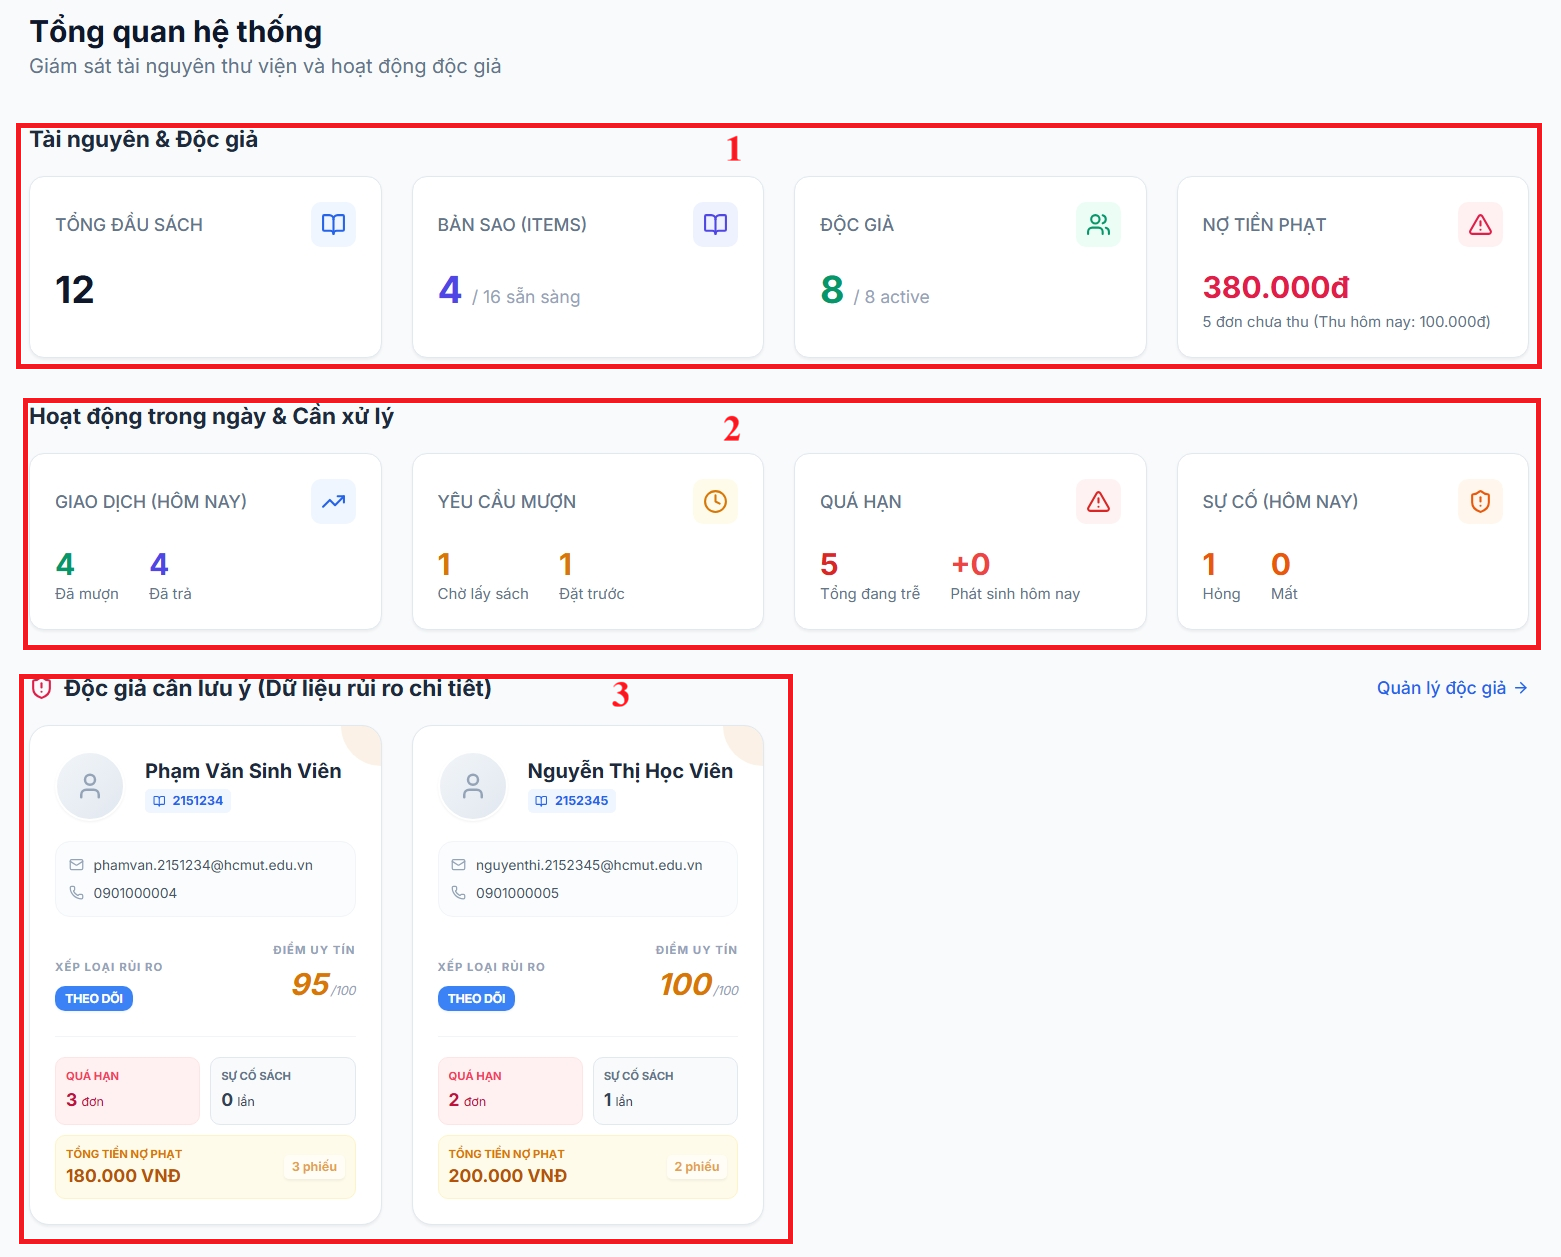
\includegraphics[width=\textwidth]{picture/dashboardthuthu/1.png}
    \caption{Giao diện trung tâm điều hành dành cho Thủ thư}
    \label{fig:librarian_dashboard}
\end{figure}

\noindent\textbf{Chú thích các vùng chức năng:}
\begin{itemize}
    \item \textbf{Vùng 1 (Hệ thống thẻ thống kê):} Cung cấp số liệu tổng hợp theo thời gian thực về quy mô kho tài liệu và người dùng, bao gồm: Tổng số đầu sách (ấn phẩm), tổng số bản sao vật lý hiện có, số lượng độc giả đang hoạt động và tổng số giao dịch mượn trả trong tháng.
    \item \textbf{Vùng 2 (Biểu đồ xu hướng mượn sách):} Trình bày dữ liệu dưới dạng biểu đồ cột, giúp thủ thư theo dõi biến động lượng mượn sách theo từng tháng trong năm. Đây là cơ sở quan trọng để đánh giá hiệu suất vận hành và nhu cầu đọc của sinh viên.
    \item \textbf{Vùng 3 (Phân tích trạng thái bản sao):} Biểu đồ tròn thể hiện tỷ lệ phân bổ trạng thái của các bản sao trong kho (Có sẵn, Đang mượn, Đang bảo trì, Thất lạc).
    \item \textbf{Vùng 4 (Hoạt động gần đây):} Danh sách các giao dịch hoặc yêu cầu đặt trước mới nhất vừa phát sinh trên hệ thống, giúp thủ thư nắm bắt nhanh các công việc cần xử lý ưu tiên.
\end{itemize}

\vspace{0.5cm}
\subsubsection{Đặc tả kỹ thuật và Xử lý dữ liệu}

Để hiển thị được các chỉ số tổng hợp trên, hệ thống sử dụng các truy vấn tính toán phức tạp (Aggregate Functions) để gom nhóm dữ liệu từ nhiều phân hệ khác nhau.

\noindent\textbf{1. Đặc tả API Thống kê tổng quát}
\begin{itemize}
    \item \textbf{Điểm cuối (Endpoint):} \texttt{GET /api/v1/librarian/dashboard/statistics}
    \item \textbf{Quyền truy cập:} Dành riêng cho quyền Thủ thư.
    \item \textbf{Mô tả logic:} Máy chủ thực hiện lệnh đếm (\texttt{COUNT}) đồng thời trên các bảng \texttt{publications}, \texttt{items}, \texttt{users} và \texttt{transactions}. Để tối ưu hiệu suất, các kết quả này có thể được lưu vào bộ nhớ đệm (Cache) và cập nhật định kỳ sau mỗi 30 phút.
\end{itemize}

\noindent\textbf{2. Đặc tả API Biểu đồ xu hướng}
\begin{itemize}
    \item \textbf{Điểm cuối (Endpoint):} \texttt{GET /api/v1/librarian/dashboard/borrow-trends}
    \item \textbf{Logic xử lý:} Hệ thống truy vấn bảng \texttt{transactions}, lọc theo trạng thái \texttt{BORROWING} và \texttt{RETURNED} trong khoảng thời gian 12 tháng gần nhất. Dữ liệu được nhóm theo tháng (\texttt{GROUP BY month}) để trả về mảng số liệu phục vụ việc vẽ biểu đồ tại giao diện.
\end{itemize}

\noindent\textbf{3. Cơ chế cập nhật thời gian thực}
\begin{itemize}
    \item Bảng điều khiển được tích hợp với hệ thống thông báo đẩy. Khi có một giao dịch mượn sách hoặc một yêu cầu đặt trước mới được thực hiện bởi độc giả, hệ thống sẽ gửi tín hiệu qua WebSocket để tự động cập nhật lại các con số thống kê trên màn hình của thủ thư mà không cần tải lại trang, giúp việc quản lý luôn ở trạng thái cập nhật nhất.
\end{itemize}


\subsection{Quản lý Bản sao }

\subsubsection{Danh sách Bản sao}

\begin{figure}[H]
    \centering
    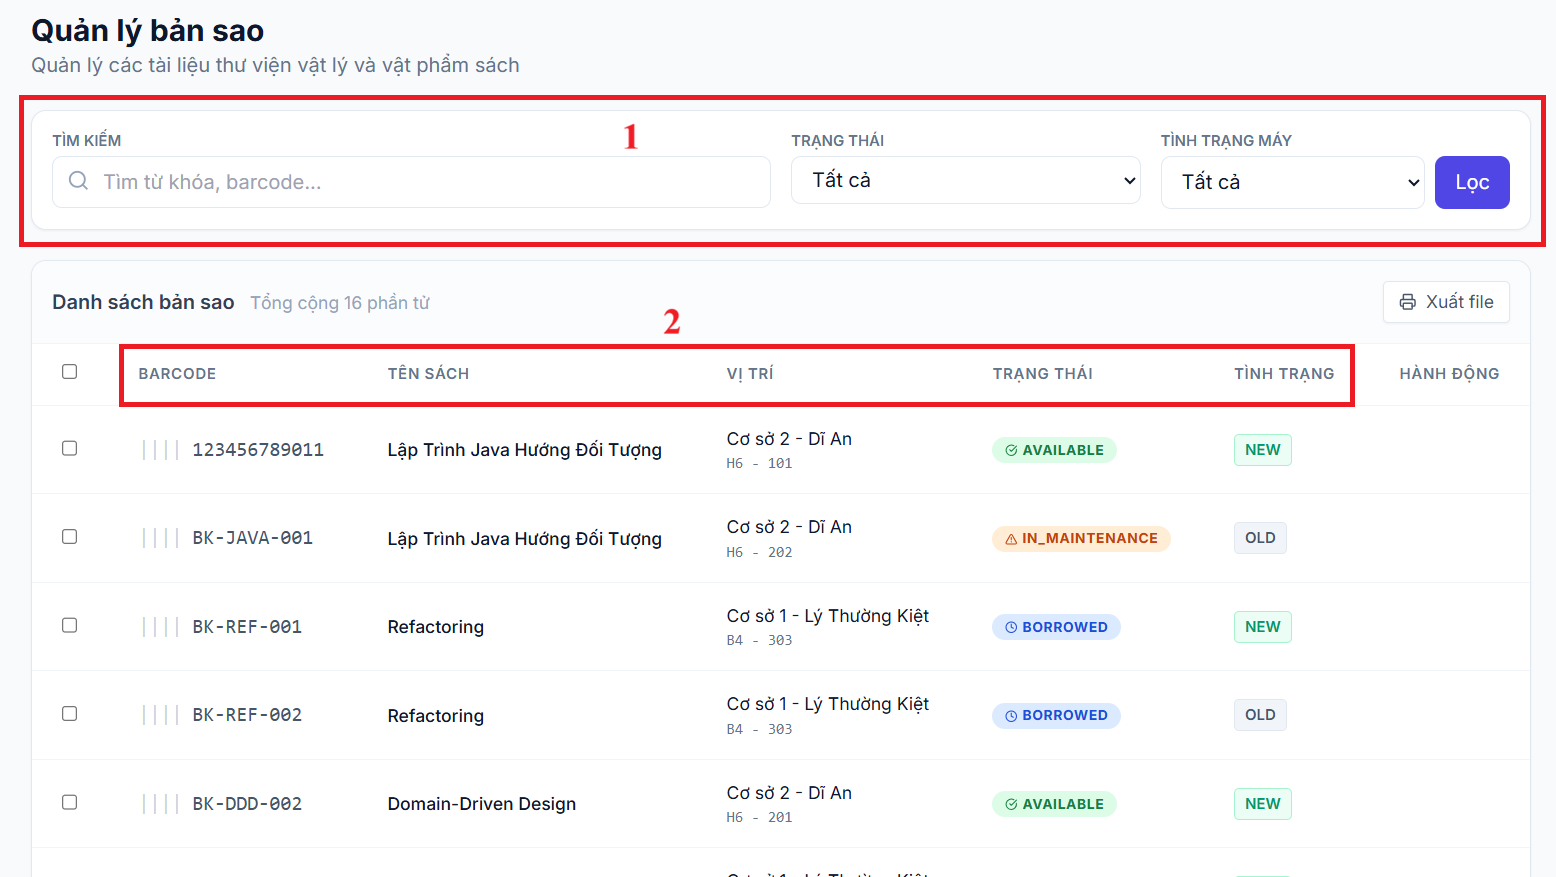
\includegraphics[width=\textwidth]{picture/bansao/1.png}
    \caption{Giao diện Danh sách bản sao trong hệ thống quản lý thư viện}
    \label{fig:list_copies}
\end{figure}

\noindent\textbf{Chú thích các vùng chức năng:}
\begin{itemize}
    \item \textbf{Vùng 1 (Bộ lọc tìm kiếm):} Cho phép tìm kiếm bản sao theo từ khóa (barcode, chi nhánh, vị trí). Người dùng có thể lọc theo trạng thái (AVAILABLE, BORROWED, RESERVED, IN\_MAINTENANCE, LOST) và tình trạng vật lý (NEW/OLD).
    \item \textbf{Vùng 2 (Bảng dữ liệu):} Hiển thị danh sách các bản sao bao gồm các trường: Barcode, Tên sách, Vị trí (Chi nhánh/Tòa/Phòng), Trạng thái và Tình trạng.
\end{itemize}

\vspace{0.5cm}
\noindent\textbf{Đặc tả API Danh sách bản sao:}
\begin{itemize}
    \item \textbf{Endpoint:} \texttt{GET /api/v1/items}
    \item \textbf{Quyền truy cập:} LIBRARIAN
    \item \textbf{Mô tả:} Lấy danh sách bản sao kèm phân trang và bộ lọc. API thực hiện truy vấn LIKE trên barcode, chi nhánh và vị trí.
    \item \textbf{Tham số truy vấn quan trọng:} \texttt{keyword} (chuỗi tìm kiếm), \texttt{status} (trạng thái bản sao), \texttt{condition} (tình trạng sách), \texttt{page} (trang hiện tại), \texttt{size} (số lượng bản ghi/trang).
\end{itemize}

\subsection{Quản lý Ấn phẩm}

Phân hệ này cho phép Thủ thư kiểm soát toàn diện danh mục tài liệu, từ việc tra cứu, phân loại đến cập nhật nội dung số của từng ấn phẩm trong hệ thống.

\subsubsection{Giao diện Danh sách Ấn phẩm}

\begin{figure}[H]
    \centering
    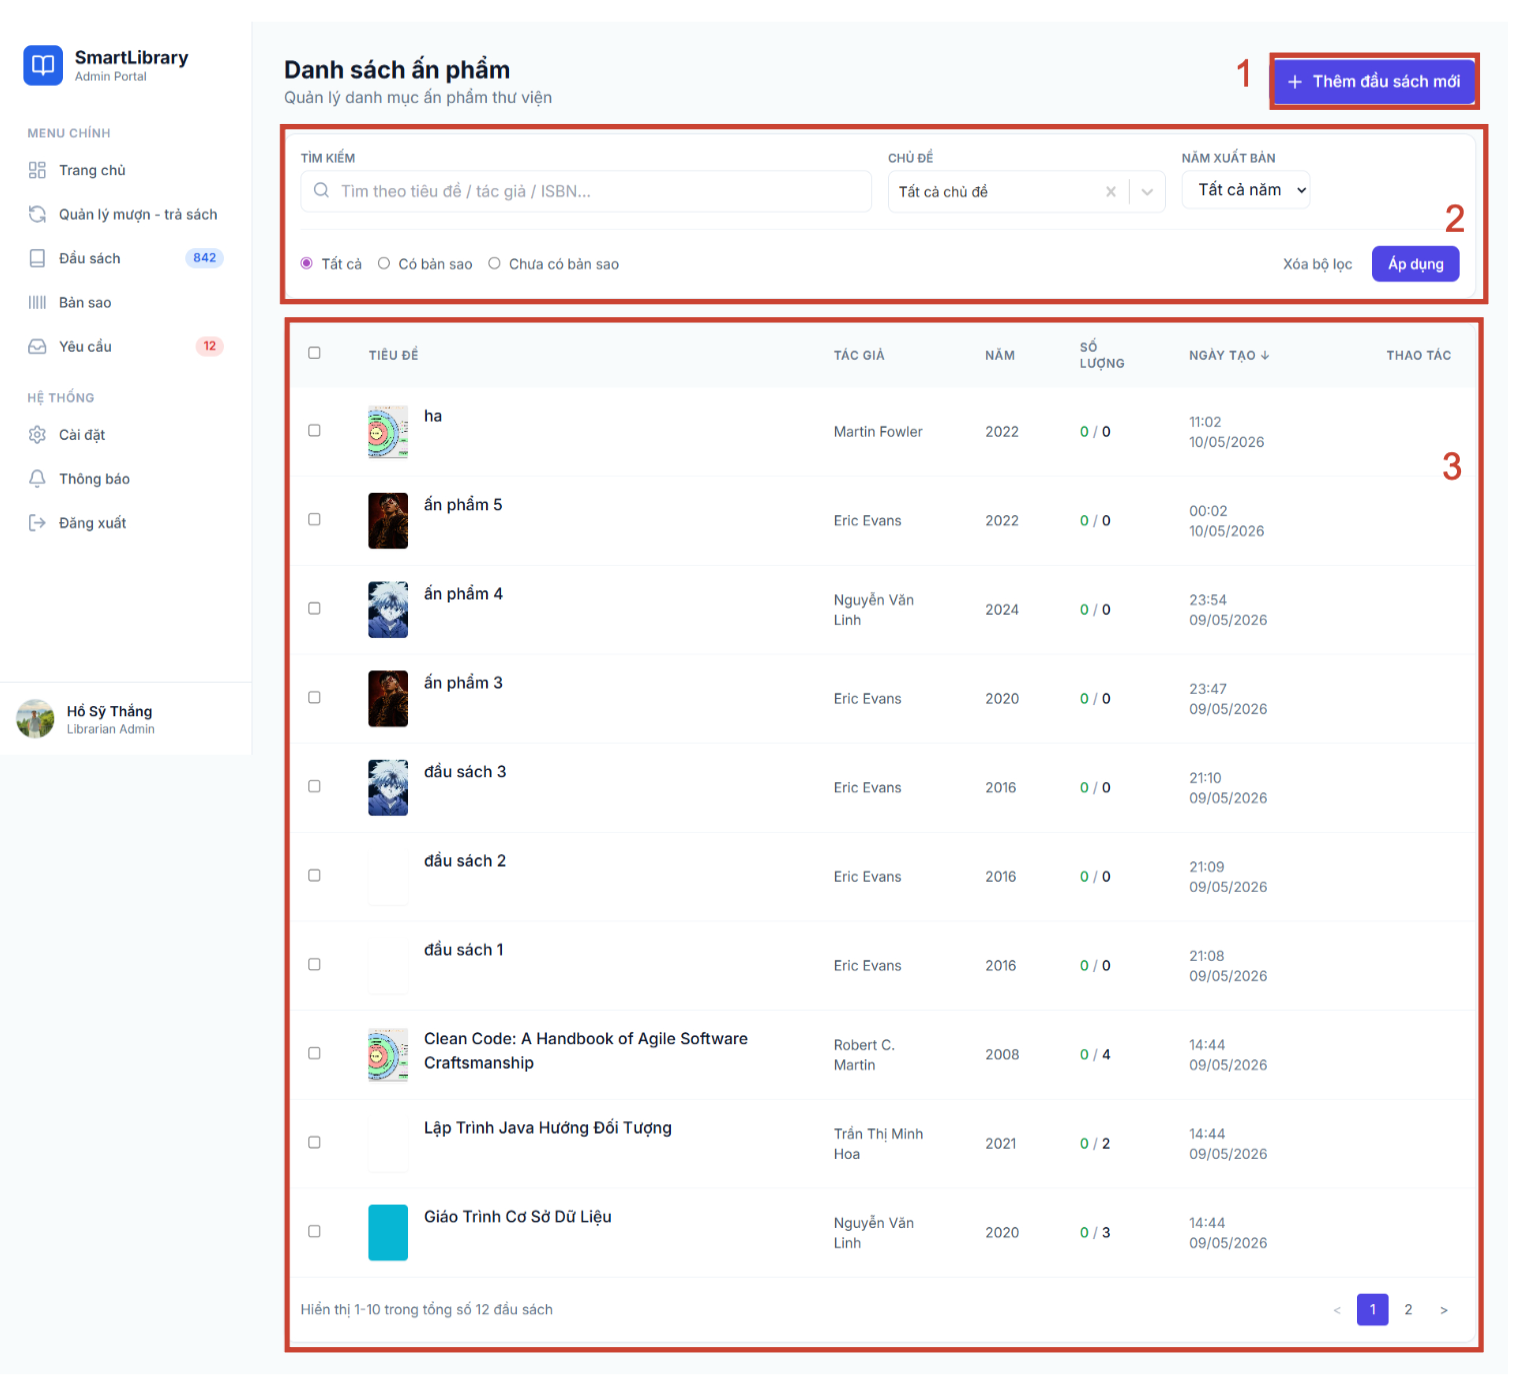
\includegraphics[width=\textwidth]{picture/quanlypublication/1.png}
    \caption{Giao diện quản lý danh mục ấn phẩm tập trung}
    \label{fig:admin_pub_list}
\end{figure}

\noindent\textbf{Các khu vực chức năng chính (Hình \ref{fig:admin_pub_list}):}
\begin{itemize}
    \item \textbf{Tìm kiếm và Thao tác:} Thanh tìm kiếm hỗ trợ tra cứu đa năng theo tiêu đề, tác giả hoặc mã ISBN. Nút "Thêm đầu sách mới" cho phép khởi tạo nhanh một ấn phẩm vào hệ thống.
    \item \textbf{Bộ lọc thông minh:} Hệ thống cung cấp các bộ lọc nâng cao theo trạng thái sở hữu (Có bản sao / Chưa có bản sao), chủ đề và năm xuất bản để tối ưu hóa việc quản lý.
    \item \textbf{Bảng dữ liệu:} Hiển thị chi tiết tiêu đề, tác giả, năm xuất bản, tỷ lệ bản sao khả dụng trên tổng số và mốc thời gian cập nhật gần nhất.
\end{itemize}

\subsubsection{Xem chi tiết và Cập nhật Ấn phẩm}

\begin{figure}[H]
    \centering
    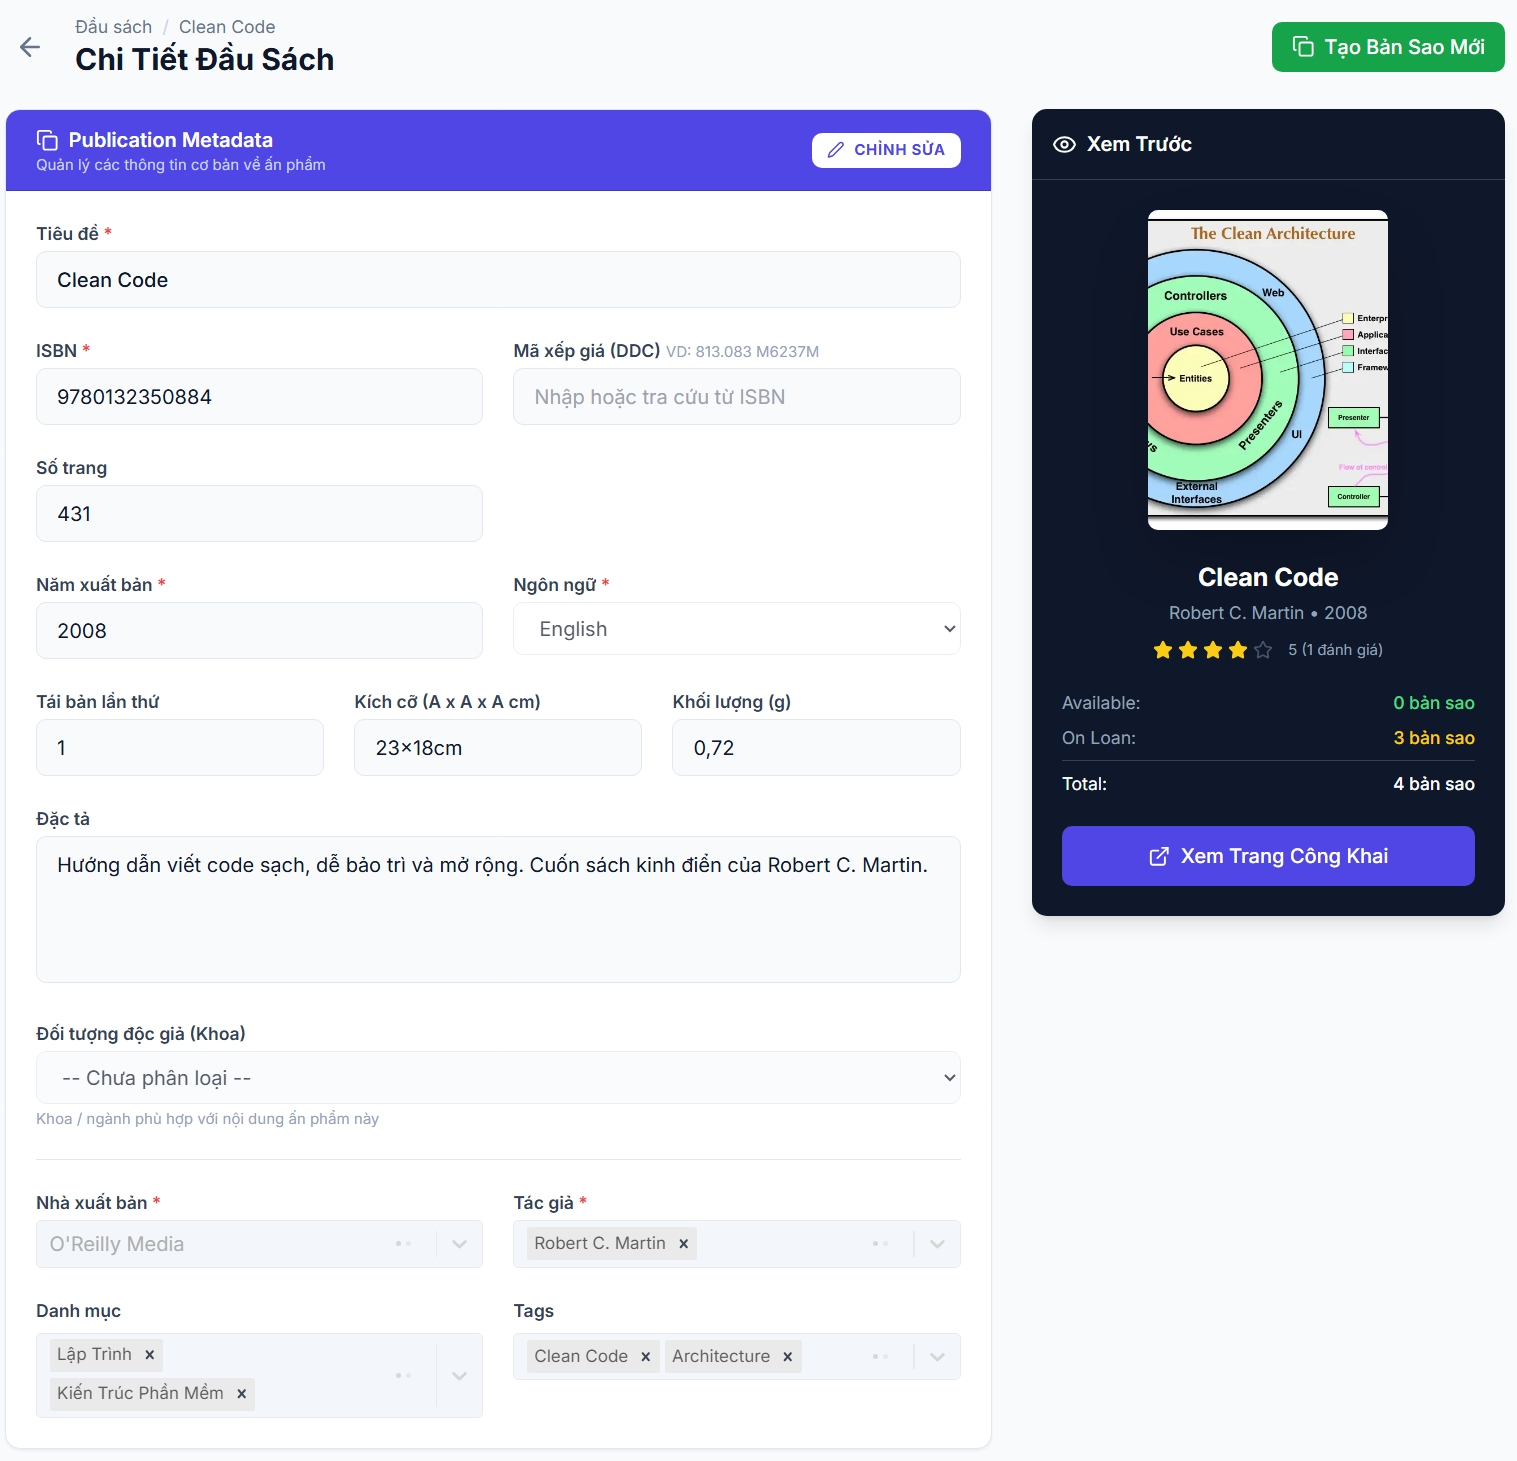
\includegraphics[width=\textwidth]{picture/quanlypublication/2giaodienxemchitietvachinhsua.jpeg}
    \caption{Giao diện hiệu chỉnh siêu dữ liệu của ấn phẩm}
    \label{fig:admin_pub_metadata}
\end{figure}

\noindent\textbf{Quản lý siêu dữ liệu (Hình \ref{fig:admin_pub_metadata}):} Thủ thư có thể hiệu chỉnh các thông tin định danh (ISBN), thông số vật lý (số trang, kích thước, khối lượng) và các thuộc tính phân loại (Tác giả, Danh mục, Tags). Hệ thống cũng cho phép thiết lập "Đối tượng độc giả mục tiêu" (Khoa/Ngành) để phục vụ thuật toán gợi ý của AI.

\begin{figure}[H]
    \centering
    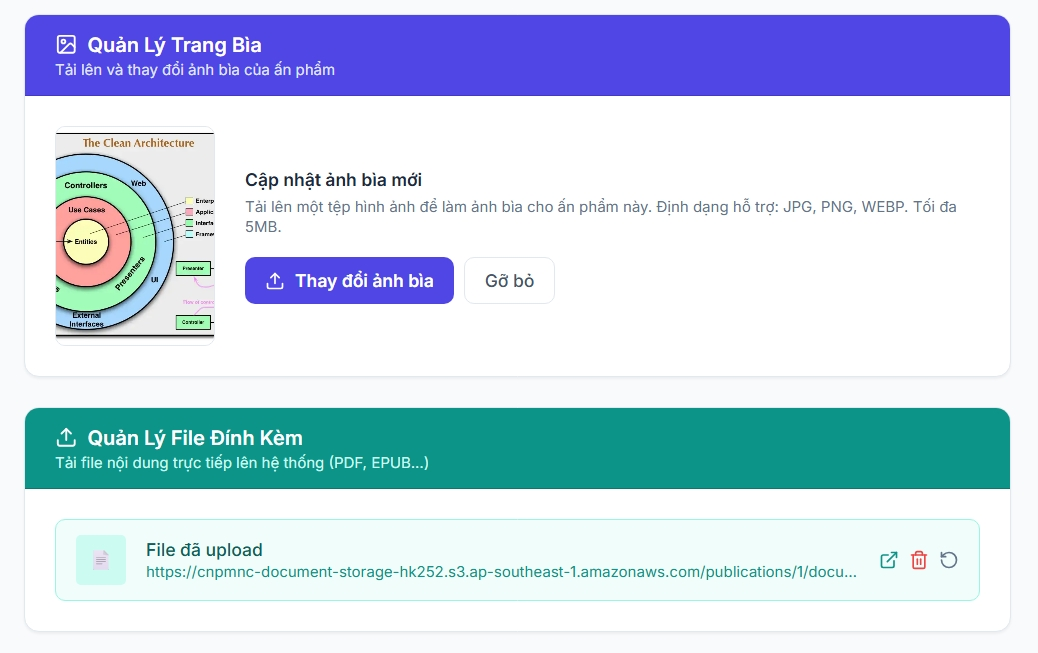
\includegraphics[width=\textwidth]{picture/quanlypublication/3giaodienxemchitietvachinhsua.jpeg}
    \caption{Quản lý ảnh bìa và tệp tin tài liệu số}
    \label{fig:admin_pub_files}
\end{figure}

\noindent\textbf{Quản lý tệp tin (Hình \ref{fig:admin_pub_files}):} Phân hệ này cho phép cập nhật ảnh bìa mới (hỗ trợ JPG, PNG, WEBP) và quản lý tài liệu số đi kèm (PDF/EPUB). Các tệp tin được lưu trữ an toàn trên dịch vụ S3.

\vspace{0.5cm}
\subsubsection{Đặc tả kỹ thuật và Xử lý dữ liệu}

\noindent\textbf{1. Truy xuất danh sách quản trị (GET API)}
\begin{itemize}
    \item \textbf{Cơ chế:} Sử dụng Native SQL với \texttt{EntityManager} để tối ưu hiệu suất khi truy vấn dữ liệu liên kết phức tạp.
    \item \textbf{Kỹ thuật:} Sử dụng hàm \texttt{STRING\_AGG} để gộp danh sách tác giả/danh mục và mệnh đề \texttt{FILTER} để đếm số bản sao khả dụng (\texttt{AVAILABLE}). Bộ lọc \texttt{hasItems} được xử lý bằng truy vấn con \texttt{EXISTS} để không làm sai lệch kết quả phân trang.
\end{itemize}

\noindent\textbf{2. Đồng bộ hóa dữ liệu cập nhật (PUT API)}
\begin{itemize}
    \item \textbf{Quy trình:} Sau khi cập nhật các thông tin cơ bản qua JPA \texttt{saveAndFlush}, hệ thống sẽ thực hiện đồng bộ các bảng trung gian.
    \item \textbf{Xử lý:} Toàn bộ các liên kết cũ (Tác giả, Thể loại, Tags) sẽ bị xóa và chèn mới hàng loạt (Batch Insert) bằng \texttt{JdbcTemplate} kết hợp với trình tạo định danh \texttt{TsIdGenerator} để đảm bảo tốc độ xử lý.
\end{itemize}

\subsection{Tạo mới ấn phẩm}

Quy trình khởi tạo một ấn phẩm mới trong hệ thống được thiết kế theo mô hình đa bước nhằm đảm bảo tính toàn vẹn của dữ liệu và tối ưu hóa băng thông máy chủ khi xử lý các tệp tin dung lượng lớn.

\subsubsection{Thiết lập thông tin siêu dữ liệu}

\begin{figure}[H]
    \centering
    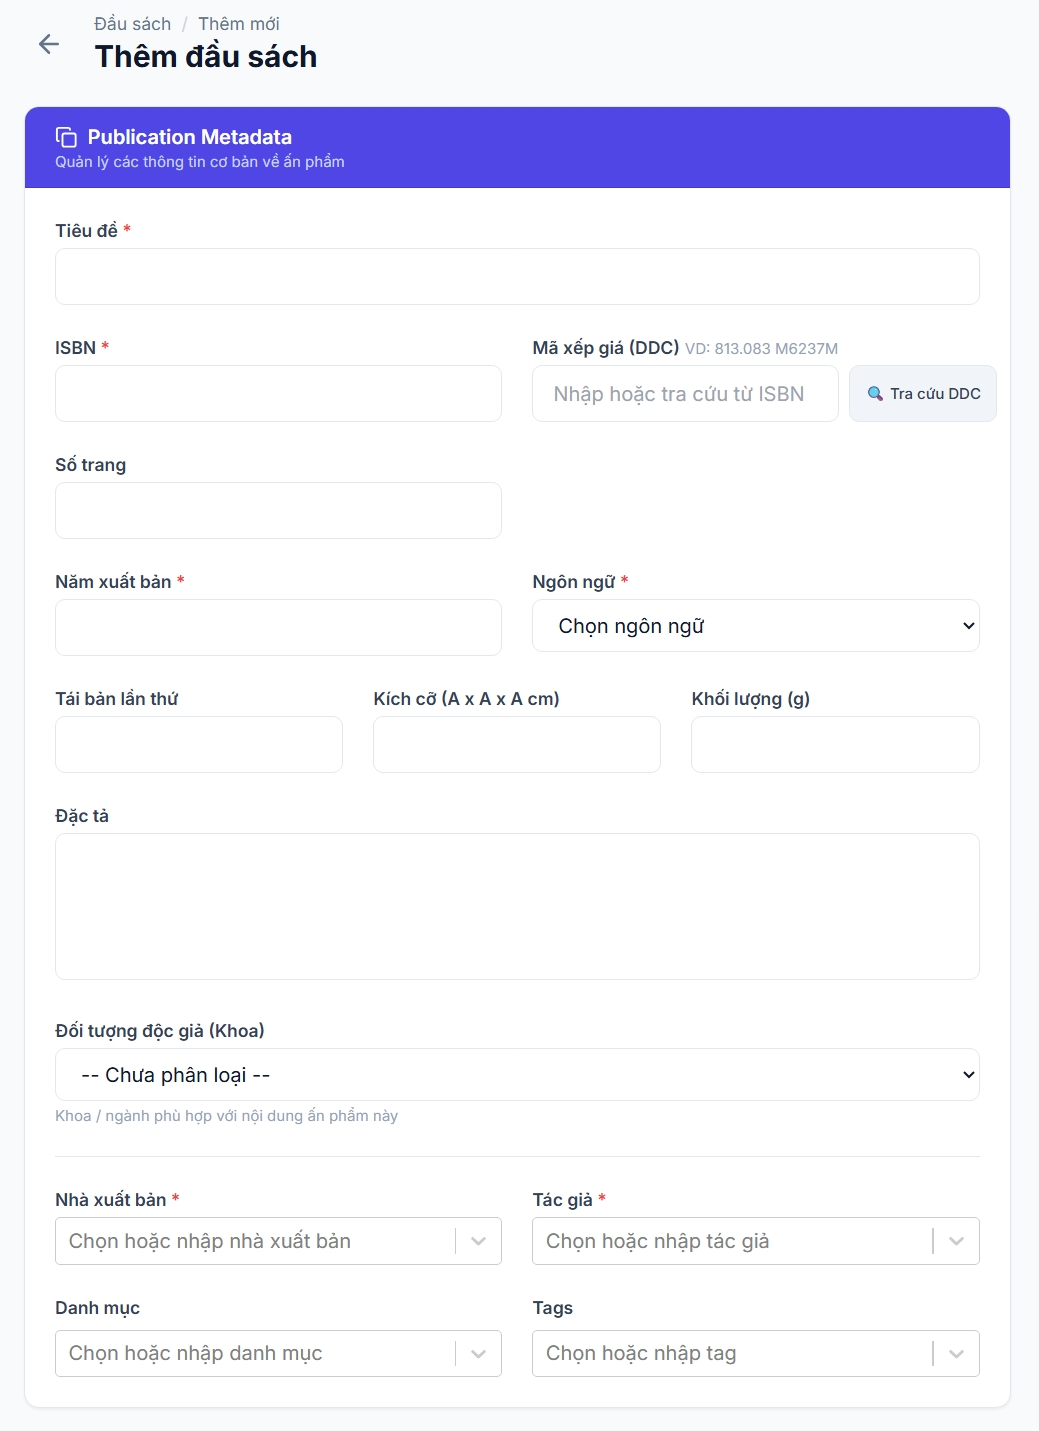
\includegraphics[width=0.85\textwidth]{picture/taomoipublication/1metadata.jpeg}
    \caption{Giao diện nhập thông tin chi tiết ấn phẩm}
    \label{fig:publication_metadata}
\end{figure}

\noindent\textbf{Chú thích các vùng chức năng:}
\begin{itemize}
    \item \textbf{Vùng 1 (Thông tin định danh):} Các trường dữ liệu cốt lõi bao gồm mã ISBN, Tiêu đề ấn phẩm và Nhà xuất bản.
    \item \textbf{Vùng 2 (Hệ thống phân loại):} Cho phép liên kết ấn phẩm với danh sách tác giả, danh mục thể loại và các nhãn (tags) từ khóa để phục vụ việc tra cứu.
    \item \textbf{Vùng 3 (Hỗ trợ AI):} Khu vực nhập tóm tắt nội dung do AI trích xuất và xác định đối tượng độc giả mục tiêu (ví dụ: Khoa Cơ khí) nhằm phục vụ thuật toán gợi ý sách.
    \item \textbf{Vùng 4 (Thông số kỹ thuật):} Các trường thông tin bổ sung như số trang, năm xuất bản và ký hiệu xếp giá (Call Number) để quản lý vị trí vật lý.
\end{itemize}

\subsubsection{Quản lý tệp tin đính kèm và Ảnh bìa}

\begin{figure}[H]
    \centering
    \begin{minipage}{0.48\textwidth}
        \centering
        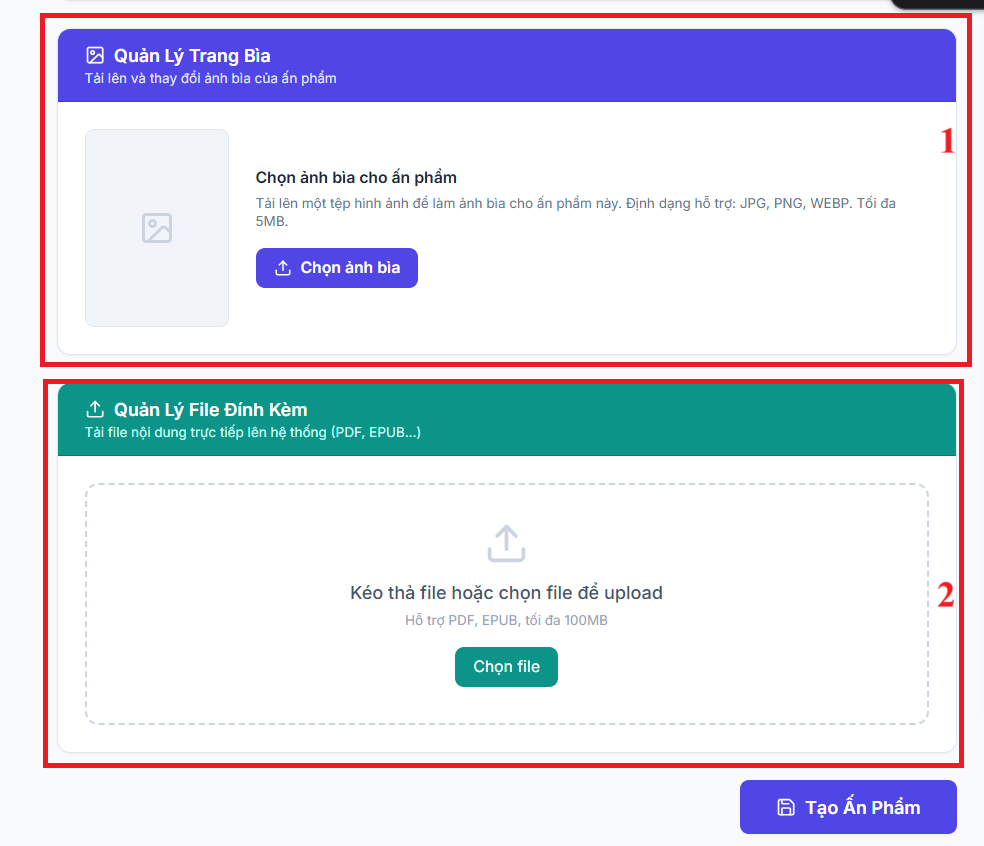
\includegraphics[width=\linewidth]{picture/taomoipublication/2uploadfileandcover.png}
        \caption{Giao diện chọn tệp đính kèm}
        \label{fig:upload_ui}
    \end{minipage}\hfill
    \begin{minipage}{0.48\textwidth}
        \centering
        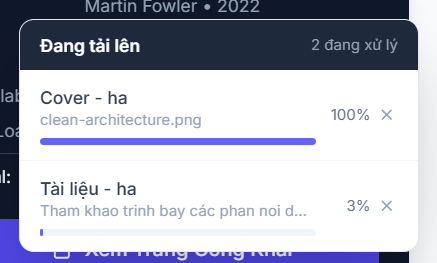
\includegraphics[width=\linewidth]{picture/taomoipublication/3uploadpanel.png}
        \caption{Bảng điều khiển trạng thái tải lên}
        \label{fig:upload_panel}
    \end{minipage}
\end{figure}

\noindent\textbf{Mô tả nghiệp vụ:} Hệ thống hỗ trợ đính kèm ảnh bìa (Cover) và tài liệu số (PDF/Ebook). Để giảm tải cho máy chủ Backend, quy trình tải lên tài liệu số được thực hiện trực tiếp từ trình duyệt lên dịch vụ lưu trữ đám mây S3 thông qua một đường dẫn được cấp quyền tạm thời (Presigned URL).

\vspace{0.5cm}
\subsubsection{Đặc tả kỹ thuật và Luồng xử lý API}

Quy trình tạo mới được thực hiện thông qua chuỗi 4 điểm cuối API tuần tự nhằm tối ưu hóa hiệu suất và khả năng mở rộng của hệ thống.

\noindent\textbf{Giai đoạn 1: Khởi tạo siêu dữ liệu (Metadata)}
\begin{itemize}
    \item \textbf{Điểm cuối:} \texttt{POST /api/v1/publications} (Quyền: Thủ thư).
    \item \textbf{Logic xử lý:} Hệ thống sử dụng \texttt{TsidGenerator} để tạo định danh duy nhất, lưu trữ vào bảng ấn phẩm và thực hiện chèn hàng loạt (batch insert) vào các bảng trung gian liên kết với tác giả và thể loại.
\end{itemize}

\noindent\textbf{Giai đoạn 2: Tải lên ảnh bìa}
\begin{itemize}
    \item \textbf{Điểm cuối:} \texttt{POST /api/v1/publications/\{id\}/cover}
    \item \textbf{Mô tả:} Tải lên tệp tin dạng \texttt{multipart/form-data}. Máy chủ xác thực định dạng ảnh (jpeg, png, webp) và dung lượng (tối đa 5MB) trước khi đẩy lên S3 tại đường dẫn \texttt{covers/\{publicationId\}/}.
\end{itemize}

\noindent\textbf{Giai đoạn 3: Cấp quyền tải tài liệu trực tiếp (S3 Bypass)}
\begin{itemize}
    \item \textbf{Điểm cuối:} \texttt{GET /api/v1/publications/\{id\}/document-upload-url}
    \item \textbf{Mô tả:} Máy chủ Backend tạo ra một mã S3 Key duy nhất và gọi S3 SDK để cấp một đường dẫn PUT tạm thời có hiệu lực trong 15 phút.
    \item \textbf{Hành động tại Giao diện:} Hệ thống Frontend nhận đường dẫn này và thực hiện lệnh \texttt{PUT} trực tiếp lên S3, giúp tiết kiệm băng thông và tài nguyên CPU của máy chủ ứng dụng.
\end{itemize}

\noindent\textbf{Giai đoạn 4: Hoàn tất liên kết tài liệu}
\begin{itemize}
    \item \textbf{Điểm cuối:} \texttt{PUT /api/v1/publications/\{id\}/document-url}
    \item \textbf{Mô tả:} Sau khi tệp đã nằm an toàn trên S3, giao diện gửi lại mã S3 Key để Backend lưu trữ vào cơ sở dữ liệu, chính thức hoàn tất việc liên kết tài liệu số với ấn phẩm.
\end{itemize}

% Preamble cần thiết: \usepackage{graphicx}, \usepackage{float}, \usepackage{tabularx}, \usepackage{booktabs}

\subsection{Nghiệp vụ Trả sách và Xử lý sự cố}

\subsubsection{Giao diện Tra cứu và Trả sách}

\begin{figure}[H]
    \centering
    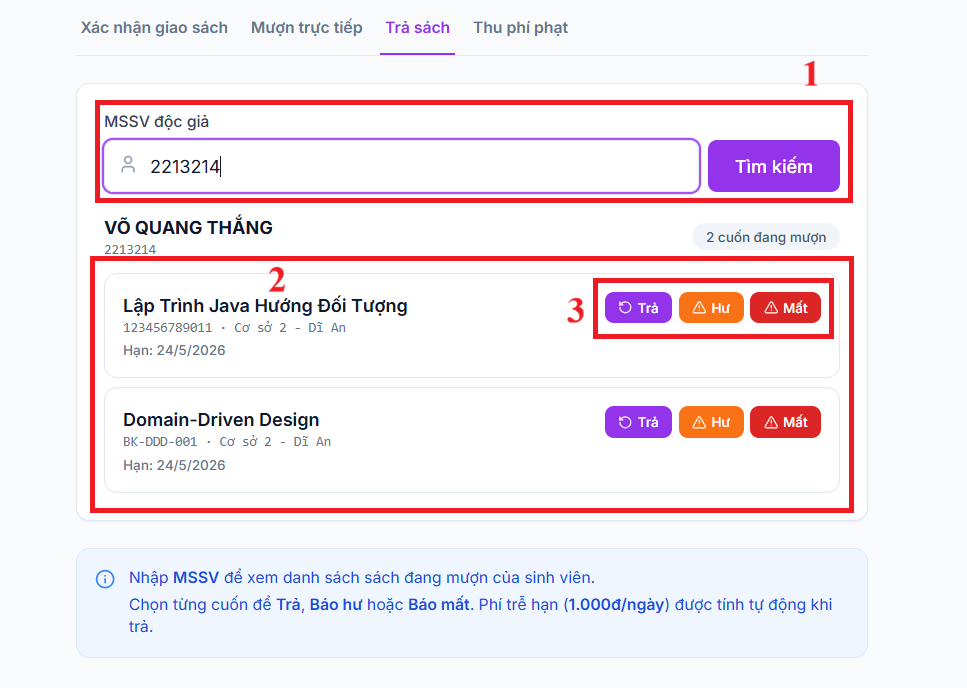
\includegraphics[width=\textwidth]{picture/trasach/1thuthunhapmssvdetracuusachdangmuon.png}
    \caption{Giao diện nhập thông tin để tra cứu sách đang mượn}
    \label{fig:return_lookup}
\end{figure}

\noindent\textbf{Chú thích giao diện:} Tại phân hệ dành cho thủ thư, hệ thống cho phép tra cứu nhanh các giao dịch đang mượn thông qua Mã số sinh viên (MSSV). Danh sách trả về hiển thị rõ các ấn phẩm mà độc giả đang giữ, đi kèm với các nút thao tác tương ứng: "Trả" (hoàn trả bình thường), "Hư" (báo cáo hư hỏng) và "Mất" (báo cáo thất lạc).

\begin{figure}[H]
    \centering
    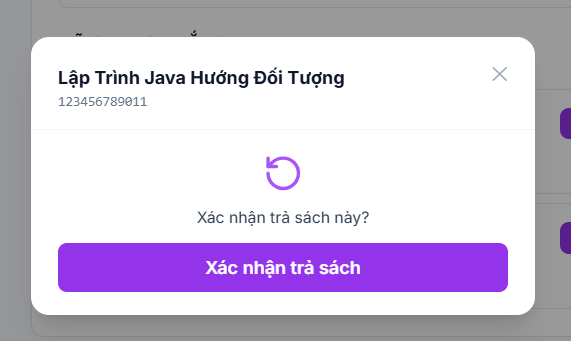
\includegraphics[width=0.6\textwidth]{picture/trasach/2popupxacnhantracuathuthu.png}
    \caption{Hộp thoại xác nhận hoàn trả tài liệu}
    \label{fig:return_confirm}
\end{figure}

\noindent\textbf{Nghiệp vụ hoàn trả cơ bản:} Khi thủ thư chọn "Trả", một hộp thoại xác nhận sẽ xuất hiện để đối chiếu thông tin sách và mã vạch lần cuối. Nếu giao dịch hoàn tất thành công, trạng thái của bản sao sẽ ngay lập tức được chuyển về "Có sẵn" (AVAILABLE). Trong trường hợp độc giả trả sách quá hạn, hệ thống sẽ tự động tính toán phí phạt dựa trên công thức số ngày trễ nhân với 1.000 VNĐ/ngày.

\subsubsection{Xử lý sự cố Hư hỏng và Mất sách}

\begin{figure}[H]
    \centering
    \begin{minipage}{0.48\textwidth}
        \centering
        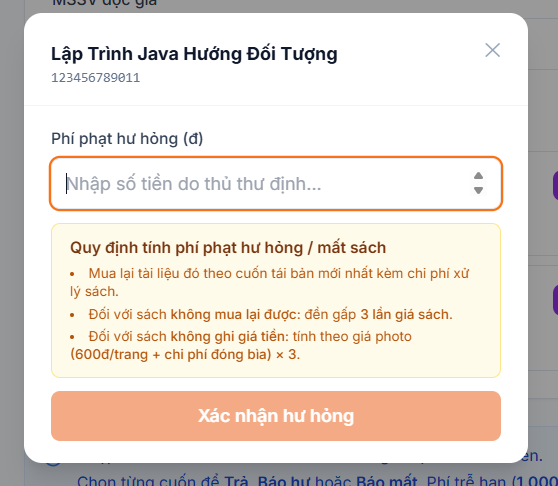
\includegraphics[width=\linewidth]{picture/trasach/3popupbaohuvasotiensinhviencanden.png}
        \caption{Hộp thoại xử lý báo cáo hư hỏng sách}
        \label{fig:return_damaged}
    \end{minipage}\hfill
    \begin{minipage}{0.48\textwidth}
        \centering
        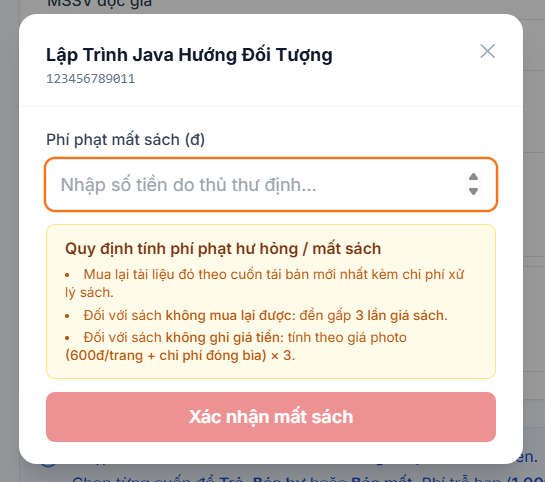
\includegraphics[width=\linewidth]{picture/trasach/4popupmatsach.png}
        \caption{Hộp thoại xử lý báo cáo mất sách}
        \label{fig:return_lost}
    \end{minipage}
\end{figure}

\noindent\textbf{Quy trình xử lý ngoại lệ:} 
Khi xảy ra sự cố vật lý với bản sao, thủ thư sẽ sử dụng tính năng "Hư" hoặc "Mất". Hệ thống cung cấp một biểu mẫu để thủ thư nhập số tiền phạt cụ thể dựa trên quy định bồi thường của thư viện (ví dụ: đền gấp 3 lần giá sách đối với sách không mua lại được). Trạng thái bản sao sẽ lập tức bị khóa, chuyển thành Đang bảo trì (IN\_MAINTENANCE) hoặc Thất lạc (LOST), đảm bảo không có giao dịch đặt trước nào được phép khởi tạo trên bản sao này.

\subsubsection{Hệ thống thông báo và Xác nhận}

\begin{figure}[H]
    \centering
    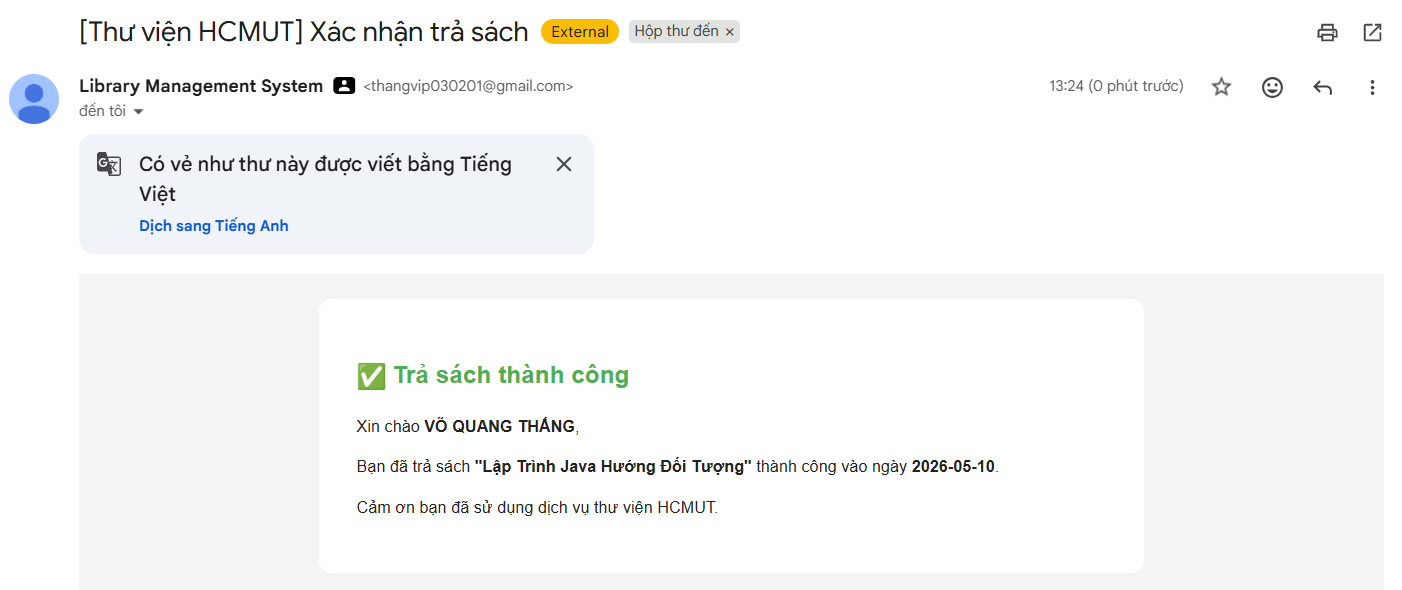
\includegraphics[width=0.9\textwidth]{picture/trasach/5guiemailxacnhanchodocgia.png}
    \caption{Thư điện tử xác nhận giao dịch trả sách thành công}
    \label{fig:return_email}
\end{figure}

\noindent\textbf{Mô tả luồng thông báo:} Ngay sau khi thủ thư xác nhận trả sách trên hệ thống, một sự kiện (event) sẽ được kích hoạt thông qua Kafka. Độc giả sẽ lập tức nhận được một thư điện tử biên nhận, ghi rõ thời gian hoàn tất giao dịch để lưu trữ và đối soát.

\vspace{0.5cm}
\subsubsection{Đặc tả API và Kỹ thuật điều phối}

Phân hệ trả sách yêu cầu xử lý logic phức tạp để đảm bảo tính nhất quán dữ liệu, đặc biệt là cơ chế khóa chống tranh chấp (Pessimistic Lock).

\noindent\textbf{1. Truy xuất thông tin giao dịch}
\begin{itemize}
    \item \textbf{Điểm cuối (Endpoint):} \texttt{GET /api/v1/transactions/active} 
    \item \textbf{Mô tả:} Hệ thống tiến hành liên kết (JOIN) các bảng dữ liệu để tìm kiếm giao dịch đang ở trạng thái Đang mượn (BORROWING) hoặc Quá hạn (OVERDUE) tương ứng với mã vạch được cung cấp.
\end{itemize}

\noindent\textbf{2. Hoàn trả tài liệu bình thường}
\begin{itemize}
    \item \textbf{Điểm cuối (Endpoint):} \texttt{POST /api/v1/transactions/return} 
    \item \textbf{Cơ chế xử lý (Logic):} Máy chủ áp dụng khóa dữ liệu (Pessimistic Lock) trên bản sao để ngăn chặn các tiến trình đồng thời. Sau khi chuyển trạng thái giao dịch thành Đã trả (RETURNED), hệ thống sẽ gọi Dịch vụ Điều phối (ReservationAssignmentService) để tự động phân bổ quyển sách này cho độc giả tiếp theo đang xếp hàng đợi.
\end{itemize}

\noindent\textbf{3. Báo cáo và xử lý sự cố}
\begin{itemize}
    \item \textbf{Điểm cuối (Endpoint):} \texttt{POST /api/v1/transactions/\{id\}/report-issue}
    \item \textbf{Mô tả:} API tiếp nhận yêu cầu cập nhật sự cố kèm theo mức phạt bồi thường do thủ thư quyết định. Nếu độc giả đồng thời trả trễ hạn và làm mất sách, hệ thống sẽ gộp cả hai khoản phạt: phí trễ hạn (OVERDUE\_RETURN) và phí bồi thường (LOST\_BOOK) thành danh sách nợ (UNPAID) trên hồ sơ sinh viên. Quy trình phân bổ sách tự động sẽ bị chặn lại hoàn toàn đối với ấn phẩm này.
\end{itemize}

\noindent\textbf{4. Bảng tổng kết trạng thái}
\begin{table}[H]
    \centering
    \caption{Trạng thái bản sao và Phí phạt tương ứng sau khi trả sách}
    \renewcommand{\arraystretch}{1.3}
    \begin{tabularx}{\textwidth}{|l|l|X|}
        \hline
        \textbf{Trường hợp thực tế} & \textbf{Trạng thái bản sao} & \textbf{Loại phí phạt phát sinh} \\ \hline
        Trả sách đúng hạn & \texttt{AVAILABLE} & Không có \\ \hline
        Trả sách trễ hạn & \texttt{AVAILABLE} & 1 khoản: \texttt{OVERDUE\_RETURN} \\ \hline
        Báo hỏng (Đúng hạn) & \texttt{IN\_MAINTENANCE} & 1 khoản: \texttt{DAMAGED\_BOOK} \\ \hline
        Báo mất (Đúng hạn) & \texttt{LOST} & 1 khoản: \texttt{LOST\_BOOK} \\ \hline
        Báo hỏng hoặc mất + Trễ hạn & \texttt{IN\_MAINTENANCE} / \texttt{LOST} & 2 khoản: Phí sự cố + \texttt{OVERDUE\_RETURN}  \\ \hline
    \end{tabularx}
\end{table}

% Preamble cần thiết: \usepackage{graphicx}, \usepackage{float}, \usepackage{tabularx}, \usepackage{booktabs}

\subsection{Nghiệp vụ Thu phí phạt}

Phân hệ này cung cấp cho thủ thư công cụ để tra cứu và thanh toán các khoản phí phát sinh từ vi phạm của độc giả. Việc hoàn tất thanh toán sẽ giải phóng các ràng buộc, cho phép sinh viên tiếp tục sử dụng toàn bộ dịch vụ của thư viện.

\subsubsection{Giao diện Tra cứu và Thanh toán}

\begin{figure}[H]
    \centering
    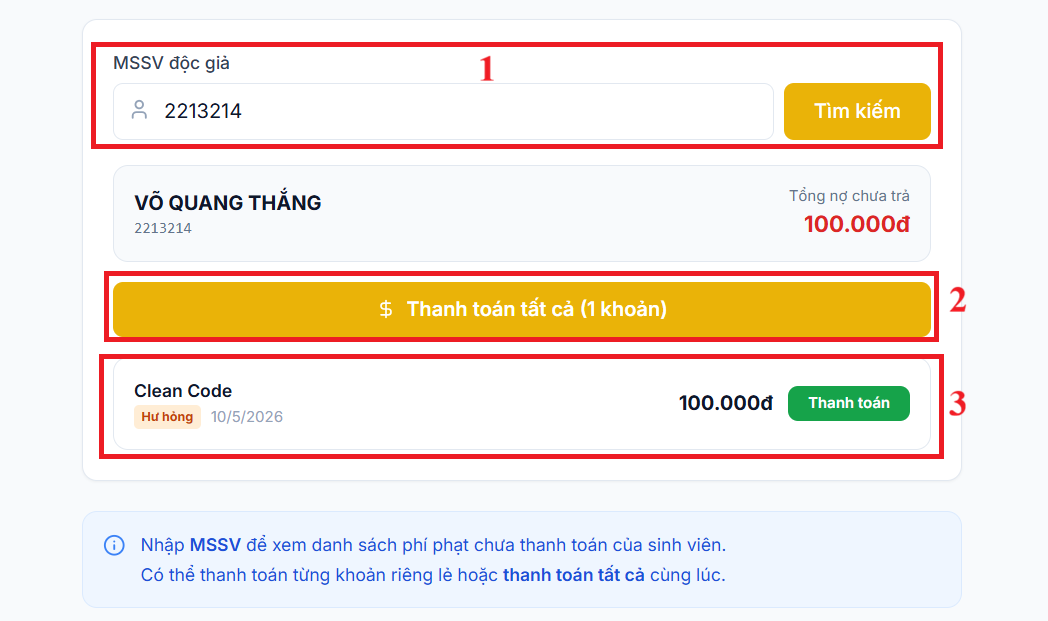
\includegraphics[width=0.9\textwidth]{picture/phiphatlibrarian/1thanhtoanphiphat.png}
    \caption{Giao diện quản lý thu phí phạt tại quầy}
    \label{fig:librarian_fine_payment}
\end{figure}

\noindent\textbf{Chú thích các vùng chức năng:}
\begin{itemize}
    \item \textbf{Vùng 1 (Khung tìm kiếm):} Thủ thư nhập Mã số sinh viên (MSSV) để hệ thống tự động truy xuất hồ sơ nợ đọng hiện tại của độc giả.
    \item \textbf{Vùng 2 (Thanh toán hàng loạt):} Nút thao tác nhanh cho phép thủ thư xác nhận thanh toán tất cả các khoản phạt cùng một lúc, tối ưu hóa thời gian xử lý khi sinh viên có nhu cầu đóng gộp nhiều khoản.
    \item \textbf{Vùng 3 (Danh sách chi tiết):} Liệt kê minh bạch từng vi phạm (ví dụ: Hư hỏng ấn phẩm) kèm theo mức phạt tương ứng và nút thanh toán cho từng khoản riêng lẻ.
\end{itemize}

\vspace{0.5cm}
\subsubsection{Đặc tả Giao tiếp API và Xử lý dữ liệu}

Quy trình thu phí phạt được tích hợp chặt chẽ với hệ thống thông báo thời gian thực nhằm đảm bảo tính minh bạch về mặt tài chính cho sinh viên.

\noindent\textbf{1. Truy xuất danh sách nợ phạt theo MSSV}
\begin{itemize}
    \item \textbf{Điểm cuối:} \texttt{GET /api/v1/fines/student}
    \item \textbf{Tham số bắt buộc:} \texttt{studentId}
    \item \textbf{Logic xử lý:} Máy chủ truy vấn thông tin người dùng. Nếu hợp lệ, hệ thống thực hiện lệnh liên kết dữ liệu (Native SQL JOIN) qua 4 bảng để lấy toàn bộ danh sách các vi phạm đang ở trạng thái chưa thanh toán (\texttt{UNPAID}).
\end{itemize}

\noindent\textbf{2. Thanh toán khoản phạt đơn lẻ}
\begin{itemize}
    \item \textbf{Điểm cuối:} \texttt{PUT /api/v1/fines/\{id\}/pay}
    \item \textbf{Logic xử lý:} Hệ thống kiểm tra định danh khoản phạt. Nếu hợp lệ, trạng thái được cập nhật thành đã thanh toán (\texttt{PAID}) cùng mốc thời gian thực thi. Ngay sau đó, một thông điệp được đẩy vào nền tảng Kafka để kích hoạt dịch vụ gửi thư điện tử (Email) xác nhận biên lai cho sinh viên.
\end{itemize}

\noindent\textbf{3. Thanh toán gộp (Bulk Update)}
\begin{itemize}
    \item \textbf{Điểm cuối:} \texttt{PUT /api/v1/fines/pay-all}
    \item \textbf{Tham số bắt buộc:} \texttt{studentId}
    \item \textbf{Logic xử lý tối ưu:} Thay vì lặp qua từng bản ghi gây hao tốn tài nguyên, hệ thống thực thi một câu lệnh \texttt{UPDATE} hàng loạt trực tiếp tại cơ sở dữ liệu. Đồng thời, hệ thống được thiết kế để chỉ kích hoạt một thông báo đẩy duy nhất tóm tắt việc thanh toán gộp, tránh tình trạng gửi thư rác (spam) làm phiền sinh viên.
\end{itemize}

\subsubsection{Quản lý Phí phạt độc giả}

Phân hệ quản lý phí phạt đóng vai trò quan trọng trong việc duy trì tính kỷ luật và bảo vệ tài sản của thư viện. Hệ thống tự động ghi nhận các khoản phí phát sinh từ vi phạm mượn trả và cung cấp giao diện minh bạch để độc giả theo dõi tình trạng tài chính cá nhân.

\paragraph{Giao diện Thống kê và Danh sách phí phạt}\mbox{}\\

\begin{figure}[H]
    \centering
    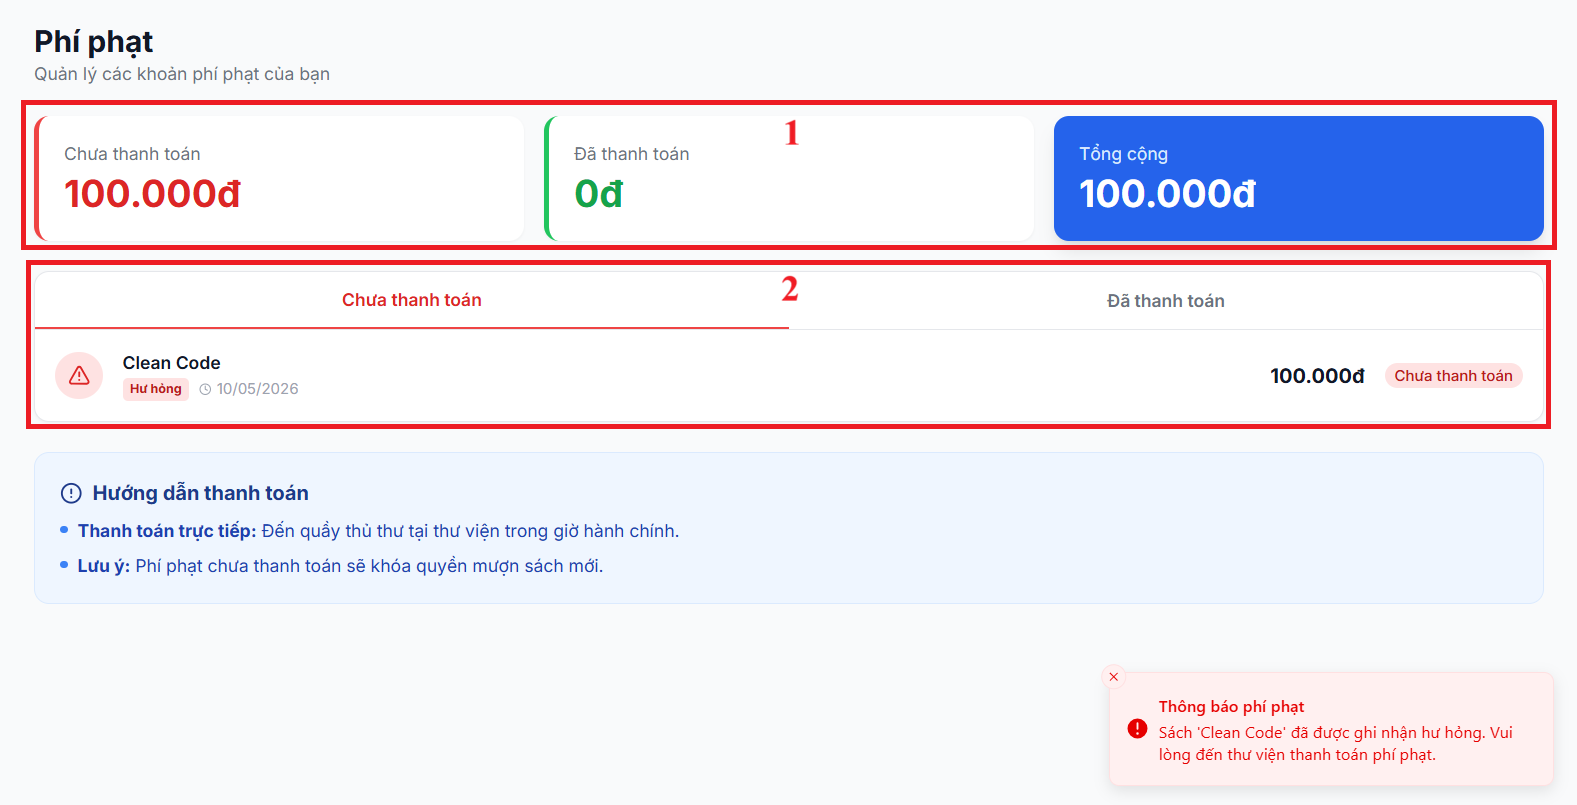
\includegraphics[width=0.95\textwidth]{picture/phiphatdocgia/1summaryvachuathanhtoan.png}
    \caption{Giao diện Thống kê tổng quát và danh sách các khoản phí chưa thanh toán}
    \label{fig:fine_unpaid}
\end{figure}

\noindent\textbf{Chú thích các vùng chức năng (Hình \ref{fig:fine_unpaid}):}
\begin{itemize}
    \item \textbf{Vùng 1 (Thẻ thống kê tổng hợp):} Hiển thị tóm tắt tình hình phí phạt thông qua các chỉ số: Tổng tiền chưa thanh toán (cảnh báo đỏ), Tổng tiền đã thanh toán (xanh lá) và Tổng cộng tất cả các khoản phí đã từng phát sinh.
    \item \textbf{Vùng 2 (Bộ lọc trạng thái):} Độc giả có thể chuyển đổi linh hoạt giữa các tab "Chưa thanh toán" và "Đã thanh toán". Khi thực hiện chuyển tab, hệ thống tự động thiết lập lại phân trang và truy vấn dữ liệu tương ứng.
    \item \textbf{Vùng 3 (Bảng danh sách chi tiết):} Mỗi dòng thông tin bao gồm tên ấn phẩm liên quan, nhãn loại vi phạm (Trễ hạn, Hư hỏng hoặc Mất sách), số tiền và ngày phát sinh.
\end{itemize}

\begin{figure}[H]
    \centering
    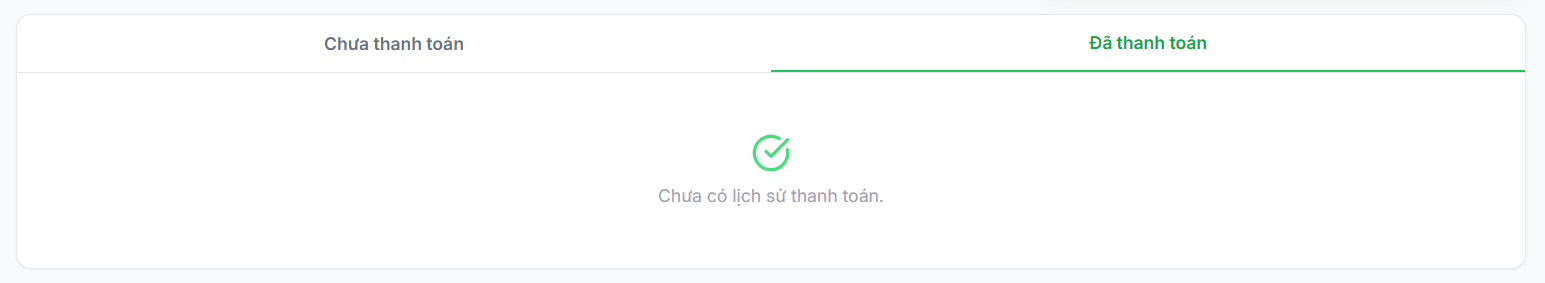
\includegraphics[width=0.95\textwidth]{picture/phiphatdocgia/2dathanhtoan.png}
    \caption{Giao diện hiển thị lịch sử các khoản phí đã hoàn tất thanh toán}
    \label{fig:fine_paid}
\end{figure}

\noindent\textbf{Mô tả nghiệp vụ:} Khi độc giả hoàn tất nộp phạt tại quầy, thủ thư cập nhật trạng thái trên hệ thống quản trị. Ngay lập tức, khoản phí sẽ được chuyển sang tab "Đã thanh toán" (Hình \ref{fig:fine_paid}) cùng với ghi nhận ngày thanh toán thực tế để độc giả đối soát.

\vspace{0.5cm}
\paragraph{Đặc tả kỹ thuật và Luồng xử lý}\mbox{}\\

Hệ thống quản lý phí phạt được tích hợp chặt chẽ với mô-đun lưu thông tài liệu để đảm bảo mọi vi phạm đều được ghi nhận tức thời.

\noindent\textbf{1. Cơ chế khởi tạo phí phạt}
\begin{itemize}
    \item \textbf{Tự động (Batch Job):} Hệ thống định kỳ quét các giao dịch quá hạn vào lúc 00:00 mỗi ngày để cập nhật phí trễ hạn (mặc định 1.000 VNĐ/ngày).
    \item \textbf{Thủ công (Librarian Action):} Khi thủ thư tiếp nhận sách trả bị hư hỏng hoặc mất, các khoản phí bồi thường sẽ được khởi tạo trực tiếp từ giao diện quản trị và ánh xạ vào hồ sơ của độc giả.
\end{itemize}

\noindent\textbf{2. Đặc tả giao tiếp API}
\begin{itemize}
    \item \textbf{Điểm cuối (Endpoint):} \texttt{GET /api/v1/fines/my-fines}
    \item \textbf{Tham số truy vấn:} \texttt{status} (UNPAID/PAID), \texttt{page}, \texttt{size}.
    \item \textbf{Logic xử lý Backend:} Hệ thống thực hiện liên kết (JOIN) giữa các bảng \texttt{fines}, \texttt{transactions}, \texttt{items} và \texttt{publications} để lấy đầy đủ thông tin tên sách và loại vi phạm dựa trên danh tính người dùng trích xuất từ mã định danh (JWT).
\end{itemize}

\noindent\textbf{3. Tối ưu hóa trải nghiệm người dùng (Frontend)}
\begin{itemize}
    \item \textbf{Tính toán tổng quan:} Ngay khi truy cập trang, hệ thống thực hiện gọi đồng thời hai yêu cầu truy vấn (cho cả trạng thái chưa trả và đã trả) để tính toán tổng số tiền hiển thị trên các thẻ thống kê phía trên, đảm bảo số liệu luôn đồng nhất.
    \item \textbf{Ràng buộc nghiệp vụ:} Một ràng buộc quan trọng được thiết lập tại tầng dịch vụ: Nếu người dùng có bất kỳ khoản phạt nào ở trạng thái chưa thanh toán (\texttt{UNPAID}), hệ thống sẽ tự động chặn mọi yêu cầu mượn sách hoặc đặt trước sách mới để đảm bảo nghĩa vụ bồi hoàn.
\end{itemize}

% Preamble cần thiết: \usepackage{graphicx}, \usepackage{float}, \usepackage{tabularx}, \usepackage{booktabs}

% Preamble cần thiết: \usepackage{graphicx}, \usepackage{float}, \usepackage{tabularx}, \usepackage{booktabs}

\subsection{Quản lý và Xem danh sách mượn trả}

Hệ thống cung cấp giao diện theo dõi hoạt động mượn trả chuyên biệt cho cả độc giả và thủ thư, giúp minh bạch hóa lộ trình lưu thông tài liệu và tình trạng của các giao dịch.

\subsubsection{Giao diện dành cho Độc giả}

Giao diện của độc giả được chia làm hai phân hệ chính thông qua hệ thống thẻ (tabs) để tối ưu hóa việc quản lý các giao dịch hiện thời và tra cứu quá khứ.

\begin{figure}[H]
    \centering
    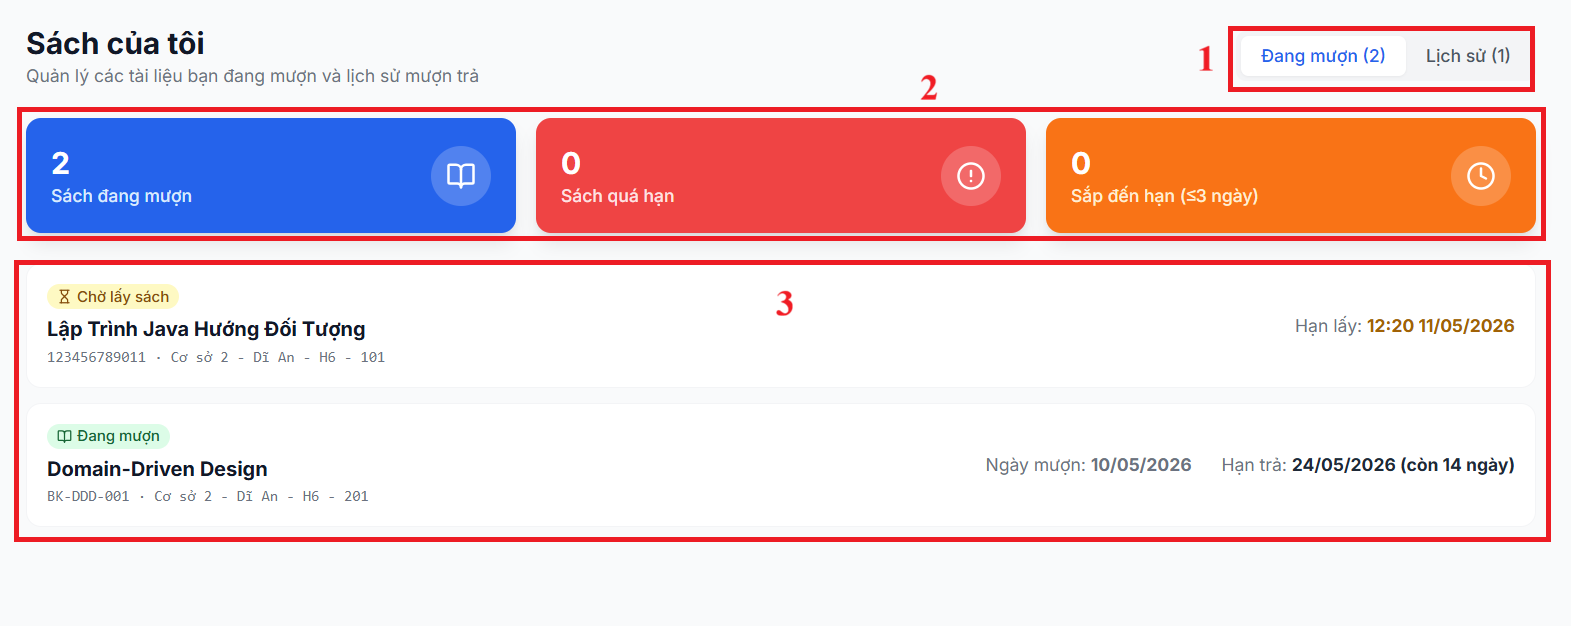
\includegraphics[width=0.95\textwidth]{picture/xemdanhsachmuon/1danhsachdangmuonvacholay.png}
    \caption{Giao diện danh sách sách đang mượn và chờ lấy}
    \label{fig:user_borrow_active}
\end{figure}

\noindent\textbf{Tab Đang mượn (Hình \ref{fig:user_borrow_active}):} 
Tập trung hiển thị các giao dịch có trạng thái \texttt{WAITING\_FOR\_PICKUP} (Chờ lấy sách), \texttt{BORROWING} (Đang mượn) và \texttt{OVERDUE} (Quá hạn). Hệ thống cung cấp các thẻ thống kê tóm tắt (Summary Cards) giúp độc giả nắm bắt nhanh số lượng sách thực tế đang giữ, số sách đã quá hạn và số sách sắp đến hạn trong vòng 3 ngày tới.

\begin{figure}[H]
    \centering
    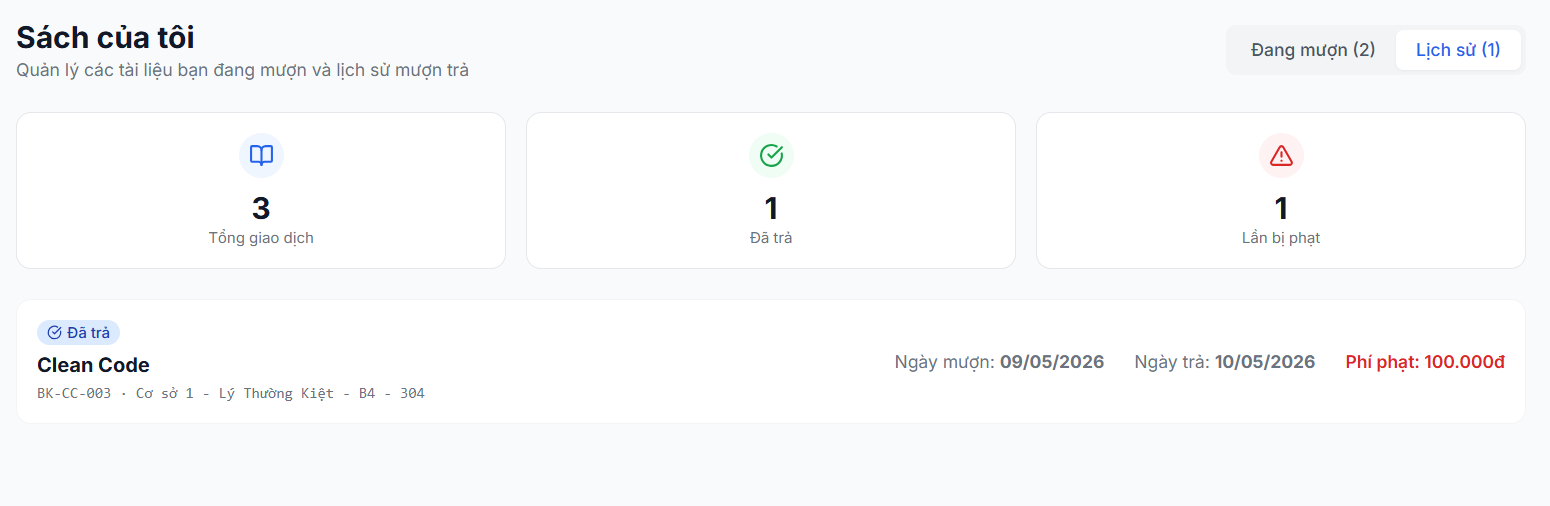
\includegraphics[width=0.95\textwidth]{picture/xemdanhsachmuon/2xemlichsumuon.png}
    \caption{Giao diện lịch sử mượn trả tài liệu}
    \label{fig:user_borrow_history}
\end{figure}

\noindent\textbf{Tab Lịch sử (Hình \ref{fig:user_borrow_history}):} 
Lưu trữ toàn bộ các giao dịch đã hoàn tất với trạng thái \texttt{RETURNED} (Đã trả) hoặc \texttt{CANCELLED} (Đã hủy). Phần thống kê tại đây tập trung vào tổng số lượt giao dịch, số lần trả sách thành công và tổng kết số lần phát sinh phí phạt (nếu có).

\begin{figure}[H]
    \centering
    \begin{minipage}{0.48\textwidth}
        \centering
        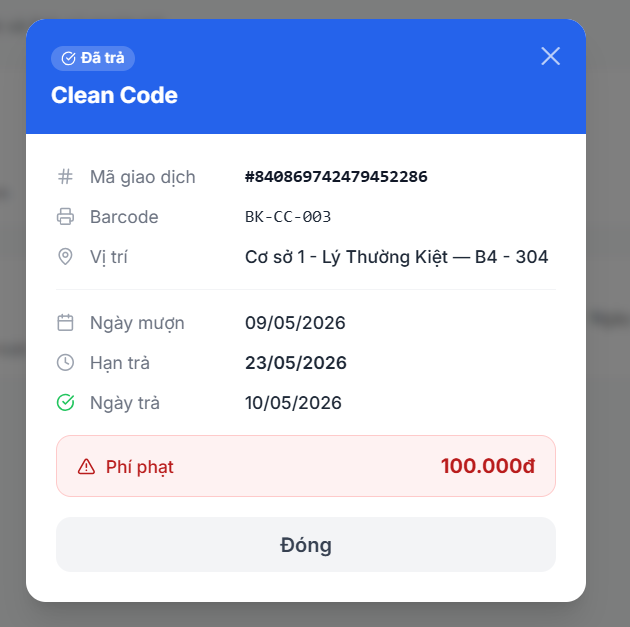
\includegraphics[width=\linewidth]{picture/xemdanhsachmuon/3xemchitietmuon.png}
        \caption{Chi tiết trạng thái giao dịch}
        \label{fig:borrow_detail_status}
    \end{minipage}\hfill
    \begin{minipage}{0.48\textwidth}
        \centering
        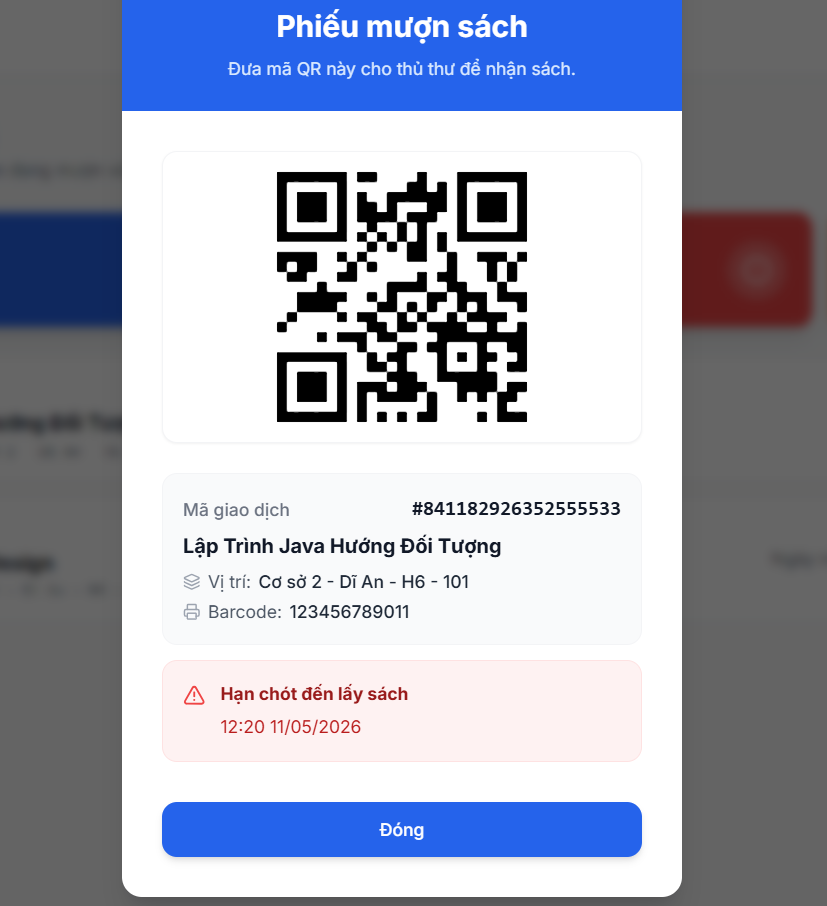
\includegraphics[width=\linewidth]{picture/xemdanhsachmuon/4xemchitietphieumuon.png}
        \caption{Thông tin biên nhận mượn sách}
        \label{fig:borrow_detail_receipt}
    \end{minipage}
\end{figure}

\noindent\textbf{Xem chi tiết giao dịch:} Khi nhấn vào từng mục, độc giả có thể xem thông tin chi tiết về bản sao (barcode, vị trí), mốc thời gian mượn/trả thực tế và lịch trình thay đổi trạng thái của phiếu mượn (Hình \ref{fig:borrow_detail_status}, \ref{fig:borrow_detail_receipt}).

\subsubsection{Giao diện dành cho Thủ thư}

\begin{figure}[H]
    \centering
    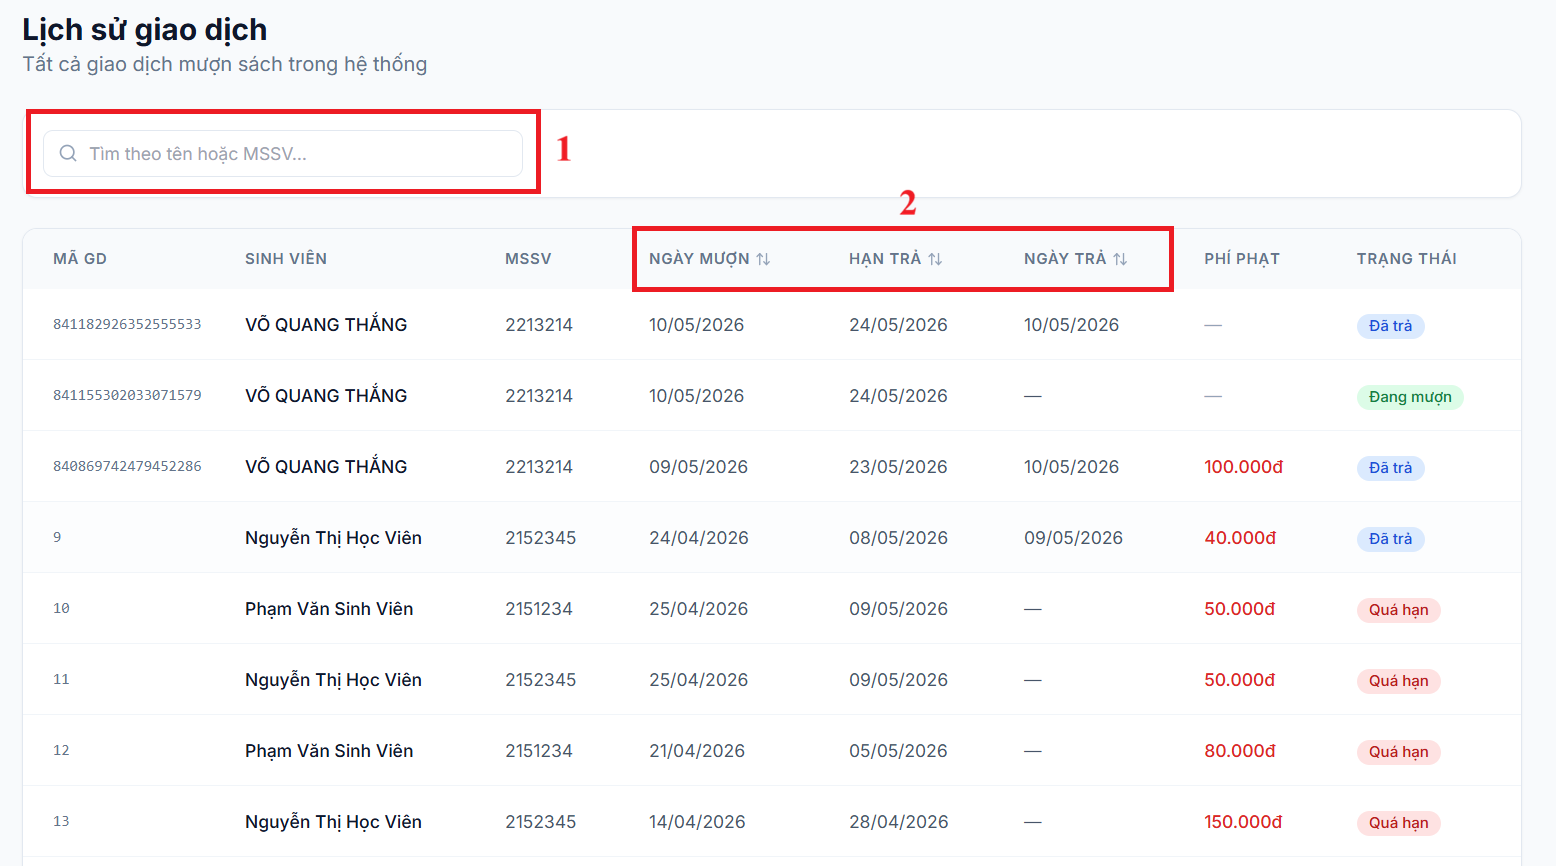
\includegraphics[width=0.95\textwidth]{picture/xemdanhsachmuon/5xemlichsumuonquahanthuthu.png}
    \caption{Giao diện quản lý danh sách mượn trả tổng thể dành cho Thủ thư}
    \label{fig:librarian_borrow_list}
\end{figure}

Thủ thư được cung cấp một bảng quản trị tập trung để theo dõi mọi biến động mượn trả trong thư viện. Bảng dữ liệu hỗ trợ hiển thị đầy đủ thông tin định danh độc giả (MSSV, Họ tên), tên ấn phẩm, thời hạn trả và mức phí phạt hiện thời của từng giao dịch (Hình \ref{fig:librarian_borrow_list}).

\vspace{0.5cm}
\subsubsection{Đặc tả API và Logic nghiệp vụ}

\noindent\textbf{1. Truy xuất danh sách mượn trả tổng quát}
\begin{itemize}
    \item \textbf{Điểm cuối (Endpoint):} \texttt{GET /api/v1/transactions} (Quyền: Thủ thư).
    \item \textbf{Cơ chế truy vấn:} Sử dụng JPQL để liên kết (\texttt{LEFT JOIN}) giữa bảng giao dịch (\texttt{BorrowingTransaction}), người dùng (\texttt{User}) và phí phạt (\texttt{Fine}) nhằm tổng hợp thông tin phản hồi đầy đủ cho giao diện danh sách. Kết quả luôn được sắp xếp theo thời gian tạo mới nhất (\texttt{createdAt DESC}).
\end{itemize}

\noindent\textbf{2. Truy xuất lịch sử theo bản sao cụ thể}
\begin{itemize}
    \item \textbf{Điểm cuối (Endpoint):} \texttt{GET /api/v1/transactions/items/\{id\}}.
    \item \textbf{Mô tả:} Phục vụ tính năng xem lịch sử mượn trả của duy nhất một quyển sách vật lý, giúp thủ thư đánh giá tần suất sử dụng và tình trạng của bản sao đó qua thời gian.
\end{itemize}

\noindent\textbf{3. Hệ thống Nhãn trạng thái (Status Badges)}
Hệ thống sử dụng bảng mã màu chuẩn để biểu thị trạng thái giao dịch một cách trực quan:
\begin{table}[H]
    \centering
    \caption{Quy ước hiển thị trạng thái mượn trả}
    \renewcommand{\arraystretch}{1.3}
    \begin{tabularx}{0.8\textwidth}{|l|l|X|}
        \hline
        \textbf{Trạng thái} & \textbf{Màu sắc} & \textbf{Ý nghĩa nghiệp vụ} \\ \hline
        \texttt{WAITING\_FOR\_PICKUP} & Vàng & Sách đang chờ độc giả đến nhận. \\ \hline
        \texttt{BORROWING} & Xanh lá & Độc giả đang giữ sách trong thời hạn cho phép. \\ \hline
        \texttt{OVERDUE} & Đỏ & Giao dịch đã vượt quá thời hạn hoàn trả. \\ \hline
        \texttt{RETURNED} & Xanh dương & Sách đã được trả về kho thành công. \\ \hline
        \texttt{CANCELLED} & Xám & Yêu cầu mượn đã bị hủy bỏ. \\ \hline
    \end{tabularx}
\end{table}


